
\chapter{System Design}\label{ch:system-design}
Laha, which means, to spread or distribute in Hawaiian, is an abstract framework for distributed sensor networks that provides a means for turning primitive data into actionable insights, tiered management of voluminous amounts of sensor data. Major goals are in part accomplished by augmenting a DSN with the ability to adaptively optimize its bandwidth, detection, classification, and sensor device power requirements.

The Laha framework is made up of five levels that can be viewed conceptually as a pyramid (see~\ref{laha-figure}). Primitive data entering the Laha framework is located at the bottom the bottom of the pyramid. As data moves upward through the levels, noise is discarded, less interesting events are discarded or aggregated into upper levels, events are given more meaning and context, and associations and predictions are made.

\begin{figure}
\caption{Laha Conceptual Model}
\centering
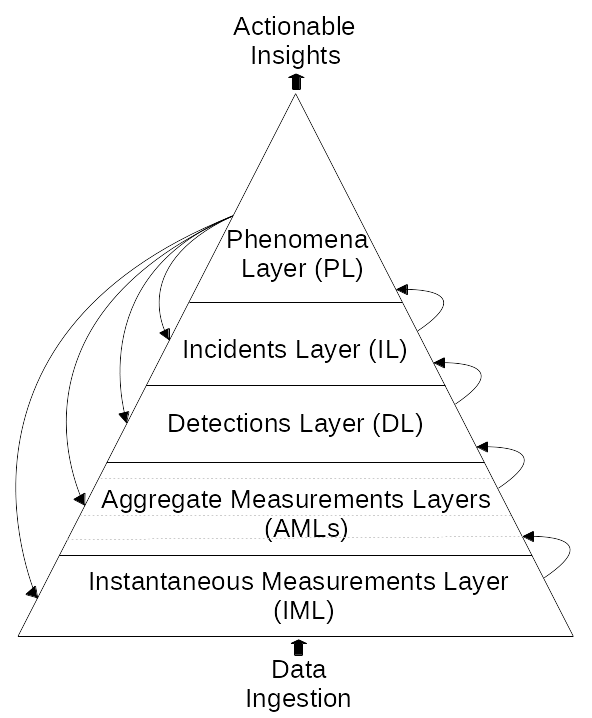
\includegraphics{figures/laha.png}
\label{laha-figure}
\end{figure}

%\section{Five proposed benefits of Laha} \label{laha-benefits}
%Laha is designed to adaptively optimize the collection, triggering, detection, and classification of signals within a DSN. These optimizations provide several benefits to DSNs. Many of these benefits can be found in other DSNs, but generally only appear as a single optimization (TODO: CITE) or as a subset of optimizations (TODO: CITE). Laha is the first DSN to combine all of these benefits for the purpose of auto-optimizing the network.

%\subsection{Tiered management of Big Data}
%% TODO If you're going to use "Big Data" as a term of art, then it needs to be rigorously defined.
%% TODO What I think you need to emphasize here is that in any Big Data scenario, you simply can't keep all the data around forever. So, what approach will be used to decide what data to keep and what data to discard?  Laha addresses this problem by having a series of levels, each with its own TTL.  This approach has the benefit of simplifying the analysis of bandwidth and storage requirements for a DSN, but at the cost of potentially discarding important data due to the "use it or lose it" design.  Part of youer evaluation should attempt to address this weakness of use it or lose it.
%
%Laha provides tiered management of the Big Data that the framework consumes. This is mainly accomplished using the layered approach that Laha provides. All data within the Laha framework is garbage collected using a configurable time to live (TTL) for each level. As data moves from the bottom to the top of the framework, noise is discarded and only interesting data as determined by the higher levels is preserved and forwarded upwards within the framework. In this way, the network can be tuned to preserve increasingly important data. One of the drawbacks of this approach is that it's possible to accidentally discard data that does contain signals of interest, but were not detectable using the current set of detection and classification algorithms. Not only does tiered management of big data increase the signal-to-noise ratio as data is moved upwards, but it also provides graceful degradation so that data pressure is never a reason a DSN is brought down. The TTL for each level can be tuned by Laha's Phenomena to either optimize for system performance or to optimize for signal analysis The details of Laha's tiered approach can be found in section \ref{big-data-management}.
%
%\subsection{Automatically provide context to classified incidents}
%% TODO This is a feature that will be hopefully much more easily evaluated once you have the two reference implementations.  I will be interested to see what kinds of contextual information are attached, and whether there are times you wished you could attach information elsewhere.
%Laha provides Annotations Phenomena (see \ref{annotations-phenomena}) that allows users or algorithms to tag signals of interest with contextual information. There is already a large amount of research for providing classifications of signals of interest, however annotations provide context about the classifications themselves. That is, Laha provides the ability to assign causality to already classified signals.
%
%Initially, a library of annotations is required to be built for a particular DSN. Once the library has been built, Laha can provide automatic annotation assignment using similarity metrics. By using annotations and determining causality, it's possible to create actionable responses to signals observed within a network.
%
%Further, annotations can be used to optimize detection and classification of known signals. For example, imagine a power quality network that observes a voltage sag on the same sensors at the same time periodically. If the cause of the voltage sag can be determined (such as a motor turning on), then detection of this signal can either be muted or analyzed more deeply. Also, other voltage sags that exhibit similar characteristics can then be automatically annotated.
%
%\subsection{Adaptive optimizations for triggering}
%% TODO This seems totally cool, but I question whether this is a novel feature. Adaptive setting of thresholds must happen in lots of different domains.  You'll want to discuss related work here, and hopefully argue that other approaches are ad-hoc and domain-specific, but the contribution of Laha is to build adaptive optimization of triggering directly into the framework as a first-class concept.
%Many triggering schemes rely on thresholds being surpassed within feature extracted data streams. For example, triggered data streams in a power quality network might consist of voltage, frequency, and THD extracted features to determine if there is likely a signal of interest observed from a given set of sensors. If any of the extracted features surpass a preset threshold, then we end up triggering the devices for raw, higher fidelity data. However, there are cases where the feature extracted stream may not surpass a predefined threshold and those sensors would not be triggered.
%
%By using different types of Phenomena, I can improve our triggering efficiency. For example, Locality Phenomena, as discussed in section \ref{locality-phenomena}, allow us to predict detections and classifications in space. If a particular grouping of sensors that are related in space always observe the same detections and classifications, then I can build a predictive model of when the framework can expect to see those things. In this way, a sensor may trigger on a passed threshold, but other sensors that are co-located may not trigger because feature extracted data is below the triggering threshold. If the Locality Phenomena predicts that other co-located sensors should have detected the same signal, then Laha might trigger those devices for high fidelity data to determine if the signal is in the raw data stream even though it didn't meet the triggering threshold.
%
%Laha can use Periodicity Phenomena, as discussed in section \ref{periodicity-phenomena}, in similar ways. When periodic signals are classified, Laha can create Future Phenomena that predicts when signals of interest should be detected and classified. This allows Laha to optimize triggering by tuning the triggers to specifically look for Periodic or Future Phenomena. Periodic and Future Phenomena also allows Laha to tune classification algorithms to the predicted classifications.
%
%\subsection{Adaptive optimizations for detection and classification}
%Not only can Laha optimize triggering, but similar usages of Locality and Future phenomena can be utilized to improve detection and classification efficiency. With Locality Phenomena, a model of common detections and classifications can be built for a set of co-located sensors. Detection and classification algorithms can be tuned to search for specific signals that are often observed within this model, pruning the search space and increasing the accuracy of detection and classification algorithms.
%
%Future and Periodic Phenomena provide the same benefits to detection and classification as Locality Phenomena. That is, if Laha is able to predict when a signal is going to arrive and also predict how that signal is going to be classified, then it can tune its detection and classification algorithms specifically for the signal of interest.
%
%\subsection{Provides a model of underlying sensor field topology}
%% TODO Either this is extremely cool, or totally frivolous, and I'm not sure which. it is frivolous if the only thing it's doing is detecting topology that you already know about (i.e. that two OPQ boxes are close together physically, but we already know that because of their lat/long coordinates.) it is totally cool if you are detecting topology that is not already known. So, it would be good to provide a specific example here for both domains (OPQ and Lokahi)
%
%Predictive phenomena use localization of signals to build communities or groupings of sensors that observe similar signals in both time and space. Over time, Laha can begin to build a model of the underlying topology of the sensing field. For instance, if a group of sensors always see the same signal, then we can assume that either the signal has a far reach, or the sensors are grouped together geographically. With enough sensor penetration, we can differentiate between these two scenarios.
%
%Further, if the sensors provide any sort of location information, Laha can provide a mapping from physical location to sensor field topology. This is especially useful when the topology of the sensor field is not known a priori. Even if we know the location of the sensors at all times, that does not mean that we understand the topology of the sensing field. For example, in a PQ network, the topology is defined by how the electrical grid is connected to itself and laid out. Laha hopes to provide a model that can determine the electrical distance between devices even if the topology of the grid is not known. As another example, take an infrasound network. It's possible that two sensors are located close to each other geographically, but if they have a large mass between them, they may not receive the same signals due to the topology of the environment around them.
%
%In this sense, Laha is not interested in knowing the location of sensors relative to each other, but is more interested in understanding how signals flow between sensors as a constraint on the topology that the signals travel through. That is, can Laha determine the statistical signal distance between sensors? And if it can, can the model be used to further tune lower levels of the Laha hierarchy?
%
%The aim is that if Laha can accurately provide a model of the underlying sensing field topology, this information can be used to optimize lower levels of the Laha hierarchy. For example, Laha can prime sensors for receiving or ignoring signals of interest by determining that a signal is supposed to arrive at a sensor before it does, i.e. Predictive Phenomena.

\section{Big Data Management in Laha} \label{sec:big-data-management}
The Laha framework acts as an adaptive sieve for filtering noise and uninteresting data collected from a DSN. In this way, each level only passes what it considers interesting to the level above it. In practice, ``higher" levels determine what is interesting and pull data from ``lower" levels. All data at a particular level is garbage collected at specific intervals relating to its important to the DSN\@.

Each level only keeps data for a specified amount of time before it is garbage collected. As data moves up the pyramid, it is generally considered more useful and therefore has a longer Time to Live (TTL), the amount of the time the data lives before it is garbage collected.  When a higher level detects ``something interesting", the data contained in the time window of ``something interesting" is copied into the levels above it and will still persist even though the original data is garbage collected. In this way, Laha preserves data from all levels if they are associated with interesting data. This also provides graceful degradation of services. The TTL is managed by the overall memory management of the system. Laha Actors are designed to work within the constraints of the TTL at different levels. If a constraint is broken, the Actor logs this issue. TTL can be optimized by Phenomena at each level to either tune for system performance or tune for decreasing of false positives and false negatives at different levels within the Laha hierarchy.

A summary of how data management in Laha is provided in Table~\ref{data-managament-table}. Note that the TTL is configurable for each implementing network and Table~\ref{data-managament-table} provides default values.

\begin{table}
	\caption{Summary of data management and context addition in Laha}
	\begin{tabular}{|c|c|c|}
		\hline
		Level & Description & Time-to-Live (TTL) \\
		\hline
		Phenomena Level (PL) & Contextual \& predictive analytics &  \\
		\hline
		Incidents Level (IL) & Classified signals &  1 year \\
		\hline
		Detections Level (DL) & Triggered windowed raw data & 1 week  \\
		\hline
		Aggregate Measurements Level (AML) & Statistical aggregates of raw data  & 1 day  \\
		\hline
		Instantaneous Measurements Level (IML) & Raw sensor data  & 1 hour \\
		\hline
	\end{tabular}
    \label{data-managament-table}
\end{table}

\subsection{Instantaneous Measurements Level}\label{subsec:instantaneous-measurements-level}
The Instantaneous Measurements Level (IML) receives raw, sampled data from the DSN. The amount of data received is determined by the sample rate of each device multiplied by the number of fields per sample. Most of the time devices in the network are mainly sampling noise. A large percentage of the data in this level is destined for garbage collection and data is assigned a Time to Live (TTL) of one hour.

\subsection{Aggregate Measurements Level}\label{subsec:aggregate-measurements-level}
The Aggregate Measurements Level (AML) is responsible for rolling up IMs from the IML. In general, this level only works with feature extracted data, rather than working with the raw samples. Each measurement in the AML provides summary statistics over a configurable time window. For example, these can include min, max, mean, median, mode, and variance statistics.

It's possible to breakup the AML into several sub levels, each with different window sizes. For example, Laha might roll IMs into one minute AMs, then roll one minute AMs into hour AMs, then days, and so on. Each sublevel within the AML can have its own configurable TTL, ensuring long term summary statistics stick around for as long as needed. This provides us a high level view of the network and can provide insights into long term trends which wouldn't be visible (or available) in the IM data stream.

Similar to IMs, AMs can be saved and copied to the levels above it when interesting data is observed. This ability allows for AMs during these time periods to be stored and saved from the garbage collection process.

At this point in the hierarchy, we are still not providing any context to the data that we are receiving. Context is provided by levels above the AML\@.

\subsection{Detections Level}\label{subsec:detections-level}
The Detections Level (DL) is the first level that provides some context to the data that the database is receiving. This level is responsible watching the feature extracted data streams, and requesting IMs from the IM level. In general, the detection level is meant to be trigger happy\footnote{Pun intended.} and be overly aggressive when determining if a feature extracted data stream looks interesting.

When a data stream looks interesting, the DL marks a timestamp $N$ seconds before the interesting features and $M$ seconds after the interesting features, where both $N$ and $M$ are configurable within the framework. The goal is to use a time window that catches signals of interest within it. Since these data ranges will be further processed and refined higher in the hierarchy, there is no issue with collecting larges amounts of data in this level.

The actual methods of detection is dependent on the characteristics of every individual sensor network. This framework assumes that the detection algorithms are provided by the implementing frameworks.

Similar to other levels, the DL level will have its IMs and AMs copied into levels above it when upper levels observe something interesting in the DL. The Detections level is set to have a TTL of a week.

\subsection{Incidents Level}\label{subsec:incidents-level}
Incidents represent classified signals. Incidents are individual classifications for signals of interest and are created by analyzing waveforms from Events. Waveforms from Events may contain multiple incidents. Individual signals may be classified as multiple incidents (for example a transient being classified as both a transient and frequency incidents).

Incidents are further analyzed to produce phenomena.

Incidents are expired after one year of storage.


\subsection{Phenomena Level}\label{subsec:phenomena-level}
Phenomena are defined as a grouping of incidents that provide one or more of annotations, locality, periodicity, predictiveness, similarity, and future phenomena.

Not only do Phenomena provide interesting insight and analytics into the underlying data, but they also provide a means for adaptively tuning the underlying collection, triggering, detection, and analysis of a distributed sensor network.

Phenomena are summarized in Table~\ref{phenomena-summary-table} and discussed in great detail in section~\ref{sec:phenomena}.

\section{Phenomena: Providing Adaptive Optimizations in Laha}\label{sec:phenomena}

\begin{table}
	\centering
	\caption{Summary of Laha Phenomena}
	\begin{tabular}{|c|c|}
		\hline
		Phenomena & Description \\
		\hline
		Annotations & Provide context about an Incident or set of incidents \\
		\hline
		Locality & Provides context on how incidents are related in time and space \\
		\hline
		Periodicity & Designation for incidents that exhibit repetitive or periodic behavior \\
		\hline
		Similarity & Subset of incidents found using grouping and community detection algorithms \\
		\hline
		Predictive & Subset of incidents characterized by predictive or forecasting models\\
		\hline
		Future & Incidents scheduled to occur in the future\\
		\hline
	\end{tabular}
	\label{phenomena-summary-table}
\end{table}

\subsection{Annotations Phenomena}\label{subsec:annotations-phenomena}
Annotations provide context about an Incident or a set of Incidents. Annotations are generally user provided or sourced from other data sources to provide supporting context to Incidents. For example, Annotations might include ``Cloud Cover", ``Hurricane Hector", ``Dryer Turns On", etc.

In some sense, annotations allow us to label our data sets beyond a simple classification and start looking at causal classifications. Once enough annotations have been assigned to classified incidents, Laha can used Annotations to attempt to label unknown incidents with similar characteristics.

Annotations are useful for creating labeled data sets. Although it is a non-goal of this dissertation to investigate the use of machine learning for signal classification and prediction, annotations provide a path for Laha-based DSNs to implement machine learning on Incidents and Events and Annotations are a useful tool for providing training data.

Annotations can be created in two ways. Either through a user interface (View in OPQ and Lokahi View in Lokahi) or algorithmically. Annotations that are created from a user interface are created by users and consumers of the DSN. This occurs when a user knows the cause of an Incident. The user can access the GUI and add an Annotation to a previously created Incident or Incidents. Users should be able to select multiple Incidents for Annotations.

The second approach to creating annotations is algorithmically. For this, we can make use of Similarity Phenomena. When new Incidents are generated, they are compared against the list of Incidents referenced by Annotation Phenomena for similarity. If the Incidents are statistically similar (with better than 75\% probability), then the newly generated Incidents will be Annotated by the same Annotation. In this case, a new Annotation Phenomena is not created, but rather the new Incidents are referenced in the original Annotation Phenomena.

Annotations can be used to tune a DSN by allowing Laha to filter on incidents with known Annotations. Users may only care about certain types of Incidents, and would prefer to filter out other types of Incidents. As an example, let's say a user of a distributed power quality network has provided an Annotation for Incidents that are generated by their solar panel installation during times of high solar radiance. This Incident may cause power issues locally and as such they are only interested in similar Incidents. The user can specify that Measurements, Trends, Events, or Incidents from their sensor should only be stored if newly created Incidents have the same Annotations that the user is interested in.

\subsection{Locality Phenomena}\label{subsec:locality-phenomena}
Locality provides context on how incidents are related to each other in both space in time. Laha is able to determine if classified incidents are local to a single sensor, to a group of co-located sensors, or global across an entire network. Sensors can be co-located in both the physical sense and also co-located within a sensing field. For example, sensors in a power quality network may be separated by large distance geographically, but co-located through the electrical grid and the grid's topology.

Over time, Locality Phenomena is used to build a model of sensors in relation to each other and to provide a statistical likelihood that co-located sensors will observe the same signal. Locality phenomena can be used to drive network triggering, detection, and classification thresholds within a distributed sensor network by using this probabilistic model for determining the likelihood that a sensor or sensors will observe a signal of interest.

The Locality of Incidents are constantly being tested. The main approach for determining the locality is combining a breadth first search (BFS) with Similarity Phenomena. When a new Incident is generated, location metadata of the sensors is used to perform a BFS of all other sensors by latitude and longitude. This is done because other sensors may have seen a similar signal of interest, but did not trigger an Event due do the signal not passing any triggering thresholds. When an Incident is triggered by a sensor or multiple sensors, for each sensor that was originally triggered a BFS is used to trigger the nearest neighbor of each of the triggering sensors. The newly triggered data is compared using Similarity Phenomena to determine if the same signal was observed in the newly triggered sensors. This process takes place recursively until sensors triggered by the BFS no longer contain the signal of interest.

If Incidents are found using this approach, Locality Phenomena is created that references all sensors that observed the same signal. These are classified as either local, semi-local, or global depending on the reach of the signal of interest.

The BFS approach works well assuming the signal topology follows the geographic topology. However, this isn't always the case. An an example, a distributed power quality network is constrained to the topology of the power grid which may now exactly match the geographic topology. One of the questions of this dissertation is to determine if a BFS approach is able to accurately identify the locality of events on networks with constrained topologies.

It is possible to determine the locality of signals on networks with constrained topologies. The Similarity Phenomena not only look at the similarity of signals by their features, but can also take into account similarity in time. In this way, Similarity Phenomena can mark Incidents as statistically similar if they not only have similar features, but also occur ``close together" in time. This approach will not find signals that do not pass triggering thresholds, but it can identify the locality of Incidents that happen on a constrained topology that would otherwise go unnoticed using the BFS approach.

By using a combination of two approaches above, I hope to show that Laha can accurately identify the locality of Incidents on both constrained and unconstrained network topologies.

By understanding the general locality of Incidents and building a statistical model of sensors that often display co-located Incidents, this Phenomena is able to tune both the sensors themselves and triggering thresholds for the network. As an example, let's say two sensors, A and B, often observe the same signals of interest, but sensor B does not pass any of the triggering thresholds for the DSN. Locality Phenomena can dynamically tune the triggering thresholds for sensor B so that it does trigger on the signals of interest that would normally go unnoticed.

Locality Phenomena can also tune the sampling rate or send rate of features from sensors. Certain signals may only be observed at certain sampling rates due to the Nyquist-Shannon sampling theorem\cite{landau1967sampling} which states that signals with a frequency $F$ can only be observed by sampling at at a rate of $2F$. Knowing that signals attenuate as a function of their distance from the source, the sampling rate of sensors can be modified to ensure that signals of interest are captured at difference distances from the signal source.

\subsection{Periodic Phenomena} \label{subsec:periodicity-phenomena}
Periodic phenomena consists of incidents that exhibit repetitive behavior, that is, the same types of incidents appearing in cycles from single or multiple devices. Periodicity allows for the easy creation of Predictive phenomena.

Periodic phenomena can come from a single incident or from multiple incidents. Periodic phenomena allow us to either tune our network to find periodic incidents or tune the  network to ignore periodic incidents depending on if the incidents are of interest. Periodic phenomena are especially useful in conjunction with Annotation phenomena as Laha can assign causality to the periodic signal.

Periodic phenomena are identified using two different approaches, a brute force approach and an approach that utilized the FFT.

The brute force approach uses the Similarity Phenomena to determine if multiple consecutive similar Incidents occur at similar time intervals. The time intervals can be anywhere on the order of seconds and go up to the order of the TTL of Incidents (that is how long Incident live in the database). An $\alpha$ parameter is used to provide the amount of uncertainty in the periodic interval and represents the absolute value of uncertainty as a percentage of the period. The $\alpha$ parameter is provided by the DSN configuration and can also be dynamically tuned by the network itself. A new Incident is marked as periodic if it is similar (as defined by Similarity Phenomena) to at least two previous Incidents and has a period $P$ between $P + (P * \alpha)$ and $P - (P * \alpha)$. When Incidents are marked as Periodic, a Periodic Phenomena is created referencing the periodic Incidents.

The second approach uses the FFT to attempt to find frequency bins on recorded Incidents. This approach computes the FFT in two phases. First, it computes the FFT over the timestamps of all Incidents. This will provide high energy in frequency bins for Incidents that occur at well defined periodic rates. Then, for each bin with energy $E_1$ above a preconfigured threshold, the Incidents in that bin are filtered for similarity using Similarity Phenomena. A second FFT is ran over the set of remaining Incidents. If the energy $E_2$ for the remaining incidents is still above the preconfigured threshold, then those Incidents are considered periodic and a Periodic Phenomena is created referencing those Incidents. Once a periodic Phenomena is created, future Incidents can be compared to the Phenomena instead of re-running the FFT over all previous incidents.

Periodic Phenomena are instrumental in creating Future Phenomena. Periodic Phenomena are used to create Future Phenomena which attempt to predict Incident arrivals at future dates. Periodic Phenomena produce Future Phenomena for all devices that are shown to be periodic. Periodic Phenomena will continue to produce Future Phenomena until consecutive Future Phenomena no longer observe the predicted signals of interest.


\subsection{Similarity Phenomena}\label{subsec:similarity-phenomena}
Similarity phenomena utilize grouping and community detection algorithms to group incidents together by their features. Common features used for grouping include time, location, incident type, incident duration, or incident features.

Similarity between signals in a DSN is a difficult problem. Signals attenuate as a function of distance from the source and the topology of the network can also change the shape of the signals. For instance, in a power quality network, signals may change as they pass through the power grid and multiple electronic components. In an infrasound DSN, signals will attenuate based on distance from the source and also change as the signals encounter physical obstacles in the environment (such as hills, man made structures, or even weather patterns).

Because of these difficulties, we can't simply correlate two signals for similarity. Instead, this Phenomena takes multiple approaches to providing statistical similarity between Incidents. The main approach that this Phenomena utilizes is comparing across high level features. These features include Incident duration and Incident classification. This Phenomena also utilizes Locality, Periodic, and Future Phenomena as weights to determine if the signals are similar. For example, if signals are periodic, then we can assume that those signals are similar. If signals are local or co-local in reference to Locality Phenomena, then it's more likely that they are similar than comparing two signals that are not generally co-located. If signals are observed from Future Phenomena, then it's more likely that they are similar to previous Incidents that were predicted using the same Phenomena.

To compare the similarity between signals, the above mentioned features are used in combination with community detection algorithms to group similar feature sets. These groupings can be further refined by correlating the signals, but due to the fact that the signal shape may change, these features are weighted less than grouping by high-level features.

K-Means clustering is used on the high-level features to create clusters of related features based on the distance from the mean values of those features. These features include a combination of Incident duration, Incident classification, Incident magnitude, and Sensor location.

From these clusters, this Phenomena creates a similarity metric. The metric is defined as $similarity = D*\alpha_1 + C\alpha_2 + M*\alpha_3 + L*\alpha_4 + Z*\alpha_5$ where $D$ is the duration metrics, $C$ is the classification metric, $M$ is the magnitude metric, $L$ is the location metric, and $Z$ is the correlation metric. The $\alpha$ values are a configurable weighting of the importance of each metric in determining similarity.


\subsection{Future Phenomena}\label{subsec:future-phenomena}
Future Phenomena are a statistical model of the likelihood of seeing an incident or incidents at future points in time. Knowing that a signal may occur with some probability allows Actor affected by those signals time to prepare for the signals.

Future Phenomena are created by a combination of other Phenomena types. The most useful Phenomena for creating Future Phenomena are Periodic Phenomena which forecasts future Incidents based off of periodicity. However, Future Phenomena also take into account other Phenomena. For instance, Future Phenomena uses Locality Phenomena to automatically trigger predicted sensors that often observe the same signals. In this way, Future Phenomena can identify signals of interest that may have not passed various triggering thresholds.

Future Phenomena also make use of Annotation Phenomena to predict signals of interest that have been Annotated. This provides actionable insights into the DSN to predict future causes of signals of interest. As an example, instead of saying that the DSN predicts a Voltage sag in a power quality network, the DSN can predict a Voltage sag due to a washer machine turning on in the future, providing more context to the DSN\@.

Future Phenomena track three items. The first is a list of sensors that should observe a signal in the future. The second is a list of future times at which a signal of interest should be observed. The final item is a statistical weight that provides the likelihood of observing a future signal of interest. The statistical weight $I$ is given as floating point value between 0 and 1 with 1 being the highest probability and 0 being the lowest probability.

Future Phenomena can also provide dynamic tuning of a DSN in multiple ways. It can either be used to tune the DSN for signals of interest, or it can be used to filter out signals that the user is not interested in. It does this by dynamically modifying the triggering thresholds of sensors that are predicted to observe a signal of interest. In most cases, this means lowering the triggering thresholds of those devices for the predictive time window, making those sensors more sensitive to the expected signal. Future Phenomena can also alter the sample rate and/or receive rate of data from the sensors themselves. The rate can be increased for the predicted time window which does increase the data load, but also decreases the time taken to observe a signal of interest.

Future Phenomena can work the other way as well by increasing triggering thresholds and decreasing sample rates for sensors that are not predicted to observe a signal of interest. In this way, we can reduce the amount of network traffic, CPU utilization, and storage requirements for the network. Of course, by doing this, we increase the odds of missing non-predictive signals of interest. This is a trade-off we are willing to make since predictive signals of interest provide more actionable information than random signals of interest.


\section{Laha Actors: Acting on the Laha Data Model}\label{sec:laha-actors:-acting-on-the-laha-data-model}
Laha Actors act on the Laha hierarchy and provide one of two functions. Actors can move data from one level of the hierarchy upwards through the hierarchy when interesting data is requested by an upper level. Actors can also apply adaptive optimizations downwards through the hierarchy. The Laha framework can support multiple actors at each level. For example, the Incidents Level in our reference power quality network contains actors for each of the following functions: IEEE classified voltage events, frequency variations, power outages, excessive THD, and many others. The Incident Level Actors move data from these incidents upwards to the Phenomena Level.

Table~\ref{laha-actors-tables} summarizes the actors that exist within the Laha framework and their purposes.

\begin{table}
	\centering
	\caption{Summary of Laha Actors}
	\begin{tabular}{|c|c|}
		\hline
		Actor & Purpose \\
		\hline
		IML Actors & Perform feature extraction and move aggregate data to AML \\
		\hline
		AML Actors & Perform triggering on data from IML, copy data to DL if interesting \\
		\hline
		DL Actors & Perform high fidelity feature extraction on possible detections \\
		\hline
		IL Actors & Perform classification and contextualization on possible detections \\
		\hline
		PL Actors & Generate predictive analytics and optimize the lower levels of the hierarchy \\
		\hline
	\end{tabular}
	\label{laha-actors-tables}
\end{table}

\subsection{Actor Constraints}\label{subsec:actor-constraints}
Actors at each level in the hierarchy are governed by a set of constraints. These constraints include the set of possible inputs, $A_i$, the set of possible outputs, $A_o$, the set of Actors it can receive data from, $A_{ai}$, the set of Actors it can transmit data to, $A_{ao}$, and a set of performance metrics that each actor must maintain, $A_p$. The constraints assigned to each Actor are determined by the hierarchy level in which the Actor resides.

Actors are responsible for reporting constraint violations and in this way, Actors are the primary provider of health, performance, and status metrics about the Laha framework.

The constraints for each level of Laha hierarchy is summarized in Table~\ref{actor-constraint-table}.

\begin{table}
	\centering
	\caption{Summary of Laha Actor Constraints at Each Level}
	\begin{tabular}{|c|c|c|c|c|c|}
		\hline
		Level & $A_i$ & $Ao$ & $A_{ai}$ & $A_{ao}$ & $A_p$ \\
		\hline
		IML & Raw samples & Aggregate trends & n/a & AML & Data ranges available \\
		\hline
		AML & Aggregate trends & Detections & IML & DL & Data ranges available \\
		\hline
		DL & Windowed waveforms & Hi-fi extracted features & AML & IL & Data \& features available \\
		\hline
		IL & Hi-fi extracted features & Contextualized incidents & DL & PL & Incident types available \\
		\hline
		PL & Contextualized incidents & Optimizations & IL & All levels & Optimizations available \\
		\hline
	\end{tabular}
	\label{actor-constraint-table}
\end{table}

\section{OPQ: A Laha-compliant Power Quality DSN}\label{sec:opq:-a-laha-compliant-power-quality-dsn}
OPQMauka is a middleware component of the Open Power Quality (OPQ) framework. The OPQ project provides a hardware and software solution for monitoring distributed power quality (PQ). The OPQ project was founded with the goal of studying how intermittent distributed renewable energy sources affect PQ not just at a user's home, but also within a user's neighborhood, between neighborhoods, and globally across the grid.

The OPQ ecosystem is made up of networked hardware sensors (OPQBoxes) and various software services (OPQMakai, OPQMauka OPQHealth, OPQView). Each of these software components are made up of individual services and plugins. The entire software system is deployed as Docker containers.

The OPQ system design is laid out in Figure~\ref{fig:opq-system}.

\begin{figure}
	\centering
	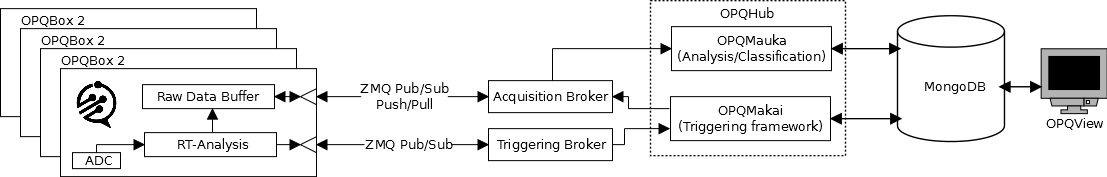
\includegraphics[width=\linewidth]{figures/system-diagram.png}
	\caption{OPQ System Diagram}\label{fig:opq-system}
\end{figure}


\subsection{OPQ: Boxes}\label{subsec:opq:-boxes}
An OPQ Box is a custom designed PQ sensor. OPQBoxes can be plugged into a wall outlet and communicate with OPQ servers using the user's WiFi connection. OPQBoxes consist of a Raspberry PI single board computer (SBC), a custom board for PQ measurements, custom firmware, and a custom enclosure. The custom board contains an ADC that samples an alternating current (AC) power signal at 12 thousand samples per second. This data is transferred to the Raspberry Pi where feature extraction and data transfer takes place. The hardware design is presented in Figure~\ref{fig:opq-box-design} and the software design is provided in Figure~\ref{fig:opq-box-software}.

\begin{figure}
	\centering
	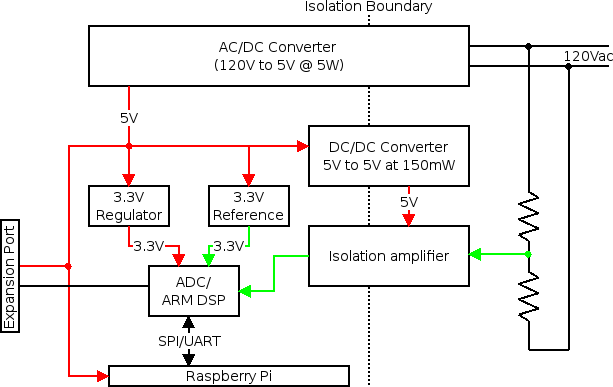
\includegraphics[width=.75\linewidth]{figures/opqbox_diagram.png}
	\caption{OPQ Box Design}\label{fig:opq-box-design}
\end{figure}

\begin{figure}
	\centering
	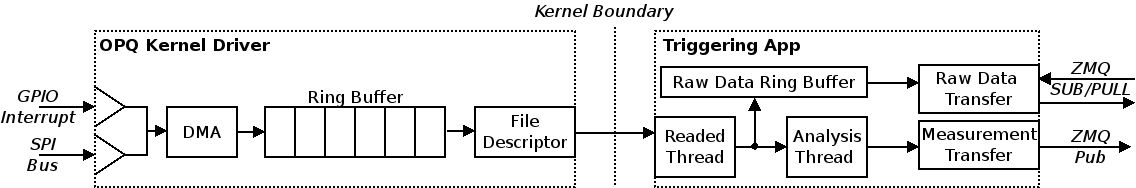
\includegraphics[width=.75\linewidth]{figures/opqbox_software.png}
	\caption{OPQ Box Software}\label{fig:opq-box-software}
\end{figure}

The feature extraction algorithms extract from the sampled waveform the following features: windowed $V_{RMS}$, frequency, and total harmonic distortion (THD) features. The feature extracted data is then sent to a central sink where further analysis is used to determine if the sensor or a subset of sensors should be triggered for raw data.

The OPQ network is a hybrid network that uses edge computing for calculating features at the edge of the network. This is opposed to networks that utilize a ``send everything" approach. In this way, Laha is able to minimize bandwidth.

OPQBoxes are synchronized to each other and the OPQ back end using the network time protocol (NTP). This provides synchronization to the millisecond level, which although is great for longer incidents, does not provide accurate timing for transients that may be shorter than tens of milliseconds.

\subsection{OPQ: Makai}\label{subsec:opq:-makai}
OPQ Makai is the central sink and triggering daemon for the OPQ framework. It is made up of several services which are responsible for aggregating and processing the measurements generated by OPQ Boxes. Low fidelity feature extracted data consisting of $V_{RMS}$, Frequency, and THD are streamed from OPQ Boxes at a configurable message rate. These data streams are observed by OPQ Makai and the daemon uses statistical methods and configurable thresholds to determine if the sensor or a subset of sensors should be triggered for a window of raw sampled waveforms.

\subsubsection{Dynamic Triggering}\label{subsubsec:dynamic-triggering}

While Makai is mostly the brain child of my colleague Sergey Negrashov, I implemented my own triggering logic into Makai to trigger for PQ events. This threshold based triggering is written as a Rust plugin for Makai's TriggeringService. The plugin receives a stream of Measurements of OPQ Boxes. Each measurement contains min, max, and average values for Frequency, Voltage, and THD over the Measurement's time window.

This plugin checks if a measurement stream from a Box passes minimum or maximum thresholds for the Measurement's features. Thresholds are provided in the Mongo database in the collection ``makai\_config". The thresholds are provided as minimum and maximum percentages from nominal. For example, the database provides values for nominal Voltage and Frequency (120$V$ and 60$Hz$ respectively) and thresholds for minimum and maximum percentage from nominal for Voltage and Frequency. It also checks the maximum percent of THD from 0.

Not only does the database provide default dynamic thresholds for all devices, but it also includes threshold overrides for individual devices. Override thresholds contain the same information as default thresholds, but also include a box\_id. When loading thresholds for a device, if an override does not exist, then default thresholds are used. If an override does exist, then the thresholds from the override are used.

All thresholds are cached for performance reasons. Values from Measurements are compared to these cached thresholds. This is needed so that this plugin does not have to request the thresholds from the database on every measurement from every Box. Instead, cached values are used. The cache is updated at a configurable interval but defaults to once a minute.

Thresholds are dynamic and can be modified by the ``ThresholdOptimizationPlugin"\ref{subsubsec:threshold-optimization-pugin} in Mauka.

This plugin utilizes a finite state machine (FSM) which maintains the triggering state for each feature for each Box. There are only two triggering states, ``TRIGGERING" and ``NOMINAL". If a feature for a Box passes a minimum or maximum threshold for a Box feature, then the state for that feature moves into the TRIGGERING state. If and when that feature is no longer passing the threshold, the state for that feature moves into the NOMINAL state and a trigger request is made for that Box which includes the time window of when that Box feature was in the TRIGGERING state.

From here, Makai handles are event storage and notification of the triggered Boxes.

Figure~\ref{fig:threshold_triggering} provides an overview of the states that are managed by the FSM\@.

\begin{figure}
	\centering
	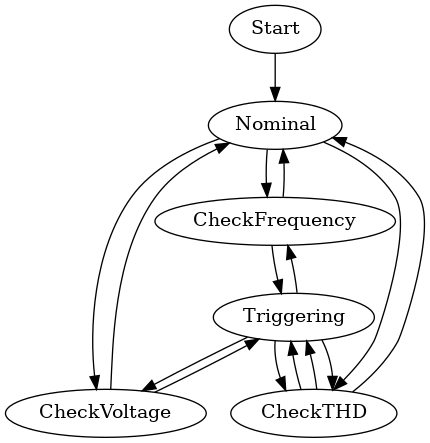
\includegraphics[width=\linewidth]{figures/threshold_triggering.png}
	\caption{Threshold Triggering FSM States}
	\label{fig:threshold_triggering}
\end{figure}

\subsubsection{TTL Provider Service}
Time-to-Live (or TTL) is a metric for defining when documents in the Mongo database should be garbage collected. The TTL metric is stored dynamically in the MongoDB collection ``laha\_config". A TTL metric is provided for each collection and the value represents the number of seconds after document creation that that document should be garbage collected. TTLs are dynamically managed by Mauka's ``TtlOptimizationPlugin"~\ref{subsubsec:ttl-optimization-pugin}. The actual garbage collection itself is provided by Mauka's ``LahaGcPlugin"\ref{sec:gc_plugin}.

TTLs are assigned in Makai to measurements, trends, and events since Makai handles storage for these collections. Because TTLs are dynamic and can be updated by Mauka at anytime, a cached TTL provider service was created to provide performant access to TTLs in the database. This service loads the TTLs from the database and caches those values for a configurable amount of time (which defaults to one minute). The cache enables Makai to assign TTLs without hitting the database for every measurement, trend, and event that it creates. If a TTL is updated by Mauka, then the cached value will expire after a configurable amount of time and the new TTL will be cached and used until the next cache invalidation.

This service lives within Makai and was written in Rust.

\subsubsection{Event Id Service}
Event ids are used to uniquely identify events produced by either Makai or Mauka. We need to ensure that event ids are unique between services and monotonically increasing. This restraint requires that a single source of truth provide the event ids to avoid race conditions between Makai and Mauka. The EventId Service is a service written in Rust that resides in Makai's Event Broker.

The service wraps an atomic integer and provides thread-safe access to this integer. The service allows anyone to peak at the current highest event id and to also increment and get the next highest available event id. When this service is initialized, it queries the MongoDB for the highest event id in the database. All other requests to this service will increment the atomic integer and use that value for the next event id. In this way, the database only needs to be queried once on initialization and all other operations are on the atomic integer.

This service can be passed directly into Makai's Event Broker using automatic reference counting (ARC). To enable Mauka to access this service, the same service is passed into a ZMQ thread using ARC. The ZMQ thread provides a ZMQ REP endpoint for requesting atomic event ids from this service. An example of Mauka requesting the event id from Makai is described in section~\ref{sec:trigger_plugin}.

A high level overview of the Event Id Service is provided if figure~\ref{fig:eid_service}.

\begin{figure}
	\centering
	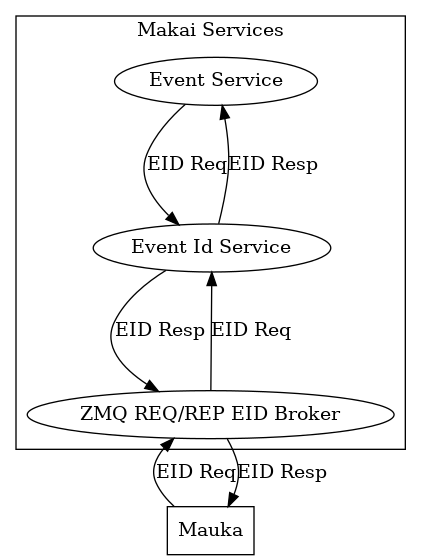
\includegraphics[width=0.7\linewidth]{figures/event_id_service.png}
	\caption{Event Id Service}
	\label{fig:eid_service}
\end{figure}

\subsection{OPQ: Mauka}\label{subsec:opq:-mauka}
OPQ Mauka (or just Mauka) is a middleware component of the OPQ system that provides higher level analytics on PQ data as well as a platform for managing data volume, providing actionable insights into the network, optimizing the network, and providing PQ based Phenomena. Most importantly, Mauka provides most of the functionality that makes OPQ a Laha-compliant DSN\@.

Mauka sits between Makai and OPQ's database. It receives messages from Makai when Makai has triggered OPQBoxes due to something interesting in the low-fidelity data stream. Mauka then retrieves the raw waveforms stored in the database by Makai, performs feature extraction, and then forwards the features and/or raw waveform to various plugins to perform classification and other high level analytics. These results are then stored in our database and presented to users in OPQView.

Mauka is written entirely in Python 3.7\cite{python:2019} and relies on various scientific libraries for analytics. These include SciPy\cite{scipy:2019}, numpy\cite{numpy}, matplotlib\cite{matplotlib}, and scikit-learn\cite{scikitlearn}. Communication between processes are accomplished with the ZeroMQ\cite{zmq} library. Messages are serialized using Protocol Buffers\cite{protobuf}. The Mauka code base consists of over 9,594 lines of Python code split over 45 Python modules. The code base is licensed under the GNU General Public License (GPL) version 3\cite{gplv3}. Mauka is hosted and publicly accessible at OPQ's github repository\cite{opqgithub}.

Mauka is designed as a distributed set of processes that communicate via type-safe message passing. Most functionality in Mauka is implemented as plugins where each plugin runs in its own process, providing horizontal scalability. The direction of communication between plugins can be modeled by a directed acyclic graph (DAG). The DAG property of Mauka plugins ensures easy horizontal scalability by making it possible to trivially create many distributed instances of plugins to meet the computational load.

The following sections will detail all components and functionality provided by Mauka.

\subsubsection{Mauka Communication}
ZeroMQ is used to facilitate communication between Mauka and Makai and also between plugins within Mauka. ZeroMQ is a light-weight message queue that provides libraries for many programming languages. ZeroMQ makes it easy to create many different types of communication topologies. However, Mauka mainly makes use of publish/subscribe and push/pull topologies. ZeroMQ is provided to Python using the pyzmq library.

In publish/subscribe, any producer can produce messages where each message contains a topic and a payload. Subscribers are then able to subscribe (or listen to) topics of interest and only ingest messages for topics that they are subscribed to.

The push/pull model on the other hand provides unidirectional message flow from a single pushed to a single puller. Using these two types of communications models in conjunction provides the entire communications backbone for Mauka.

To facilitate communication between Mauka and Makai and between Mauka plugins, two communications brokers are provided. Brokers are separate processes whose only jobs are to manage moving typed messages from a source destination to multiple target destinations.

The first broker, the Makai Event Bridge broker, is responsible for subscribing to a ZeroMQ endpoint provided by Makai. This bridge is used to pass event ids created by Makai into Mauka, alerting Mauka to the presence of new data in the database to analyze. When the message is received by the broker, it is transformed into a Mauka Message and published to the second broker, the Mauka Pub Sub Broker, and then broadcast to any subscribing plugins. Mauka plugins that subscribe to event ids then use the event id to look up the associated raw waveforms in the database to perform analysis.

The second broker, the Mauka Pub Sub broker facilitates message passing between all other parts of the Mauka ecosystem. All messages in this system are published to this broker, and all plugins subscribe to topics provided by this broker. In essence, this broker is used to route type safe messages between distributed components of this system. By using pub/sub and a broker, the plugins only need to worry about one communication endpoint instead of knowing exactly where each plugin lives in the network and how to address it individually.

Figure~\ref{fig:mauka_brokers} provides a high level view of how the brokers facilitate communication between Makai and Mauka as well as between Mauka plugins.

\begin{figure}
	\centering
	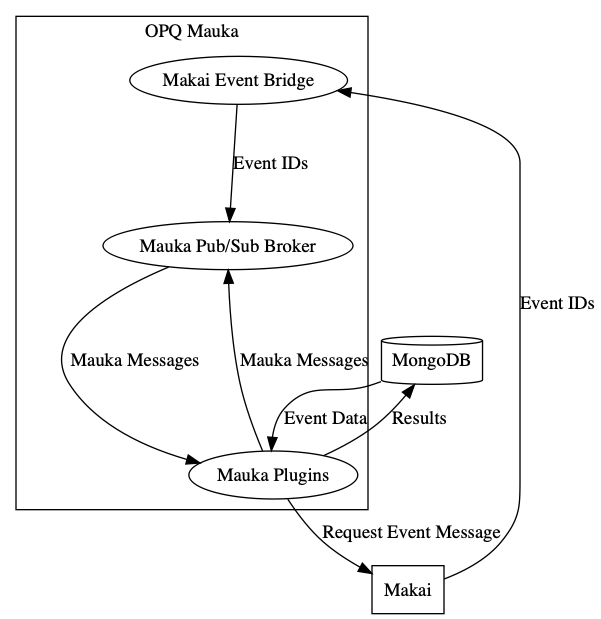
\includegraphics[width=\linewidth]{figures/mauka_brokers_communication.png}
	\caption{OPQ Mauka Brokers Communication Diagram}
	\label{fig:mauka_brokers}
\end{figure}

One down side to this approach is that the brokers become single points of failure. I believe that this issue is minimized by using the production proven ZMQ backend for communications. I have also never experienced failures in the broker during data collection or normal system usage.

\subsubsection{Mauka Communication Protocol}
The messages that are passed over ZeroMQ are serialized using the type safe protocol buffers (v3) format. Protocol buffers provide efficient binary serialization/deserialization routines for structured data and can be used from a multitude of programming languages.

Mauka provides a single message type, ``MaukaMessage", that includes many subtypes. All messages passed within Mauka are of the instance MaukaMessage and may include different subtypes. The MaukaMessage protocol is described in detail in the following tables.

The ``MaukaMessage" (Table~\ref{table:MaukaMessage}) type contains a timestamp, source, and a union type which can contain multiple types of type safe messages. Every plugin within Mauka sends and receives MaukaMessages and the plugin is responsible for checking the type of the ``message" field and acting on it.

\begin{table}[H]
	\centering
	\caption{MaukaMessage}
	\begin{tabular}{|c|p{6cm}|c|}
		\hline
		Field & Type & Description  \\
		\hline
		timestamp\_ms & uint64 & Timestamp of message creation.  \\
		\hline
		source & string & Name of plugin that produced this message. \\
		\hline
		message & oneof (Payload, Heartbeat, MakaiEvent, Measurement, MakaiTrigger, Laha, TriggerRequest, ThresholdOptimizationRequest, RateOptimizationRequest, TtlOptimizationRequest, Request) & A union of subtypes. \\
		\hline
	\end{tabular}
	\label{table:MaukaMessage}
\end{table}

The ``Payload" (Table~\ref{table:Payload}) variant of message contains data payloads cast to 64-bit precision floating point numbers. This allows us to work with data of multiple type by assuming all data payloads can be cast to 64-bit floats. This message also contains metadata relating to where the data came from, timing information, and a type safe enumeration describing the type of data stored in the payload.

\begin{table}[H]
	\centering
	\caption{Payload}
	\begin{tabular}{|c|c| p{8cm} |}
		\hline
		Field & Type & Description  \\
		\hline
		event\_id & uint32 & Event that this payload originated from.  \\
		\hline
		box\_id & string & Box that this payload originated from. \\
		\hline
		data & [f64] & An array of data cast to double precision floats. \\
		\hline
		payload\_type & PayloadType & Enumeration providing payload type information. \\
		start\_timestamp\_ms & uint64 & Start timestamp of first payload element \\
		\hline
		end\_timestamp\_ms & uint64 & End timestamp of last payload element\\
		\hline
	\end{tabular}
	\label{table:Payload}
\end{table}

The ``PayloadType" (Table~\ref{table:PayloadType}) variant is an enumeration that describes the type of data stored in any provided payload.

\begin{table}[H]
	\centering
	\caption{PayloadType}
	\begin{tabular}{|c|c| p{8cm} |}
		\hline
		Field & Enum Value & Description  \\
		\hline
		ADC\_SAMPLES & 0 & ADC waveform samples from the Box.  \\
		\hline
		VOLTAGE\_RAW & 1 & Raw waveform voltage obtained by dividing ADC values by a calibration constant. \\
		\hline
		VOLTAGE\_RMS & 2 & RMS waveform obtained by dividing raw voltage by sqrt(2). \\
		\hline
		VOLTAGE\_RMS\_WINDOWED & 3 & RMS extracted feature array. \\
		\hline
		FREQUENCY\_WINDOWED & 4 & Frequency extracted feature array. \\
		\hline
	\end{tabular}
	\label{table:PayloadType}
\end{table}

The ``Heartbeat" (Table~\ref{table:Heartbeat}) variant is a message that is periodically sent from each plugin providing statistics about plugin health.

\begin{table}[H]
	\centering
	\caption{Heartbeat}
	\begin{tabular}{|c|c|p{8cm}|}
		\hline
		Field & Type & Description  \\
		\hline
		last\_received\_timestamp\_ms & uint64 & Last time a plugin on\_message was fired.  \\
		\hline
		on\_message\_count & uint32 & The amount of times on\_message has been fired. \\
		\hline
		status & string & Custom status message that plugin can override. \\
		\hline
	\end{tabular}
	\label{table:Heartbeat}
\end{table}

The ``MakaiEvent" (Table~\ref{table:MakaiEvent}) variant is a message which includes the ``event\_id" of a newly created event from Makai. This message is received by the ``MakaiEventPlugin" and is used to begin processing new events within Mauka generated by Makai.

\begin{table}[H]
	\centering
	\caption{MakaiEvent}
	\begin{tabular}{|c|c|p{8cm}|}
		\hline
		Field & Type & Description  \\
		\hline
		event\_id & uint32 & The event number that Makai has recorded.  \\
		\hline
	\end{tabular}
	\label{table:MakaiEvent}
\end{table}

The ``Measurement" (Table~\ref{table:Measurement}) variant is a message that contains an instantaneous measurement which includes a timestamp, Voltage, Frequency, and THD metrics.

\begin{table}[H]
	\centering
	\caption{Measurement}
	\begin{tabular}{|c|c|p{8cm}|}
		\hline
		Field & Type & Description  \\
		\hline
		box\_id & string  & Box that this measurement came from. \\
		\hline
		timestamp\_ms & uint64 & Timestamp that this measurement was recorded. \\
		\hline
		frequency & double & The instantaneous frequency of this measurement. \\
		\hline
		voltage\_rms & double & The instantaneous RMS voltage of this measurement. \\
		\hline
		thd & double & The instantaneous THD of this measurement. \\
		\hline
	\end{tabular}
	\label{table:Measurement}
\end{table}

The ``MakaiTrigger" (Table~\ref{table:MakaiTrigger}) variant is a message type that is used to send to Makai in order for Mauka to trigger boxes for raw data. This is used when Mauka sees something interesting and wishes to request more data than what was originally provided by Makai.

\begin{table}[H]
	\centering
	\caption{MakaiTrigger}
	\begin{tabular}{|c|c|p{8cm}|}
		\hline
		Field & Type & Description  \\
		\hline
		event\_start\_timestamp\_ms & uint64  & The start timestamp of the trigger. \\
		\hline
		event\_end\_timestamp\_ms & uint64 & The end timestamp of the trigger. \\
		\hline
		event\_type & String & A string description of the event (or reason) we are triggering boxes. \\
		\hline
		max\_value & double & The maximum value of ``event\_type" observed in the triggering stream. \\
		\hline
		box\_id & String & The OPQBox id. \\
		\hline
	\end{tabular}
	\label{table:MakaiTrigger}
\end{table}

The ``Laha" (Table~\ref{table:Laha}) message variant contains multiple types of messages all relating to Laha. These include messages for managing TTL, garbage collection, and Laha based statistics.

\begin{table}[H]
	\centering
	\caption{Laha}
	\begin{tabular}{|c|c|p{8cm}|}
		\hline
		Field & Type & Description  \\
		\hline
		laha\_type & Oneof (Ttl, GcTrigger, GcUpdate, GcStat) & Sum type that contains multiple subtypes. \\
		\hline
	\end{tabular}
	\label{table:Laha}
\end{table}

The ``Ttl" (Table~\ref{table:Ttl}) Laha message variant is used to dynamically specify TTLs for the provided collection.

\begin{table}[H]
	\centering
	\caption{Ttl}
	\begin{tabular}{|c|c|p{8cm}|}
		\hline
		Field & Type & Description  \\
		\hline
		collection & String & The data collection type that should have its TTL updated.  \\
		\hline
		ttl\_s & uint32 & The number of seconds that a collection should have its TTL set to. \\
		\hline
	\end{tabular}
	\label{table:Ttl}
\end{table}

The ``GcTrigger" (Table~\ref{table:GcTrigger}) variant is a message that is sent to the GC plugin to notify it that GC should be performed on the domains specified in the message.

\begin{table}[H]
	\centering
	\caption{GcTrigger}
	\begin{tabular}{|c|c|p{8cm}|}
		\hline
		Field & Type & Description  \\
		\hline
		gc\_domains & [GcDomain] & The data collection type that should have its TTL updated.  \\
		\hline
	\end{tabular}
	\label{table:GcTrigger}
\end{table}

The ``GcDomain" (Table~\ref{table:GcDomain}) enum is used to specify a garbage collection domain within Laha.

\begin{table}[H]
	\centering
	\caption{GcDomain}
	\begin{tabular}{|c|c| p{8cm} |}
		\hline
		Field & Enum Value & Description  \\
		\hline
		MEASUREMENTS & 0 & Laha measurements.  \\
		\hline
		TRENDS & 1 & Laha trends. \\
		\hline
		EVENTS & 2 & Laha events. \\
		\hline
		INCIDENTS & 3 & Laha incidents. \\
		\hline
		PHENOMENA & 4 & Laha Phenomena. \\
		\hline
		SAMPLES & 5 & Laha samples. \\
		\hline
	\end{tabular}
	\label{table:GcDomain}
\end{table}

A ``GcUpdate" (Table~\ref{table:GcUpdate}) variant is a message that informs the GC plugin to update the TTL for a particular document and all documents living under it.

\begin{table}[H]
	\centering
	\caption{GcUpdate}
	\begin{tabular}{|c|c|p{8cm}|}
		\hline
		Field & Type & Description  \\
		\hline
		from\_domain & GcDomain & The GcDomain from which this update originated. All collections under this domain are also updated.  \\
		\hline
		id & uint32 & The id of the document that should have its TTL updated. \\
		\hline
	\end{tabular}
	\label{table:GcUpdate}
\end{table}

A ``GcStat" (Table~\ref{table:GcStat}) variant message is a message that contains statistics on the number of items garbage collected from a particular GcDomain.

\begin{table}[H]
	\centering
	\caption{GcStat}
	\begin{tabular}{|c|c|p{8cm}|}
		\hline
		Field & Type & Description  \\
		\hline
		gc\_domain & GcDomain & The GcDomain from which this statistic originated. \\
		\hline
		gc\_cnt & uint64 & The count of items garbage collected on the last GcTrigger message.  \\
		\hline
	\end{tabular}
	\label{table:GcStat}
\end{table}

A ``TriggerRequest" (Table~\ref{table:TriggerRequest}) variant message is a message that is instantiated by Phenomena and sent to the ``TriggerPlugin" enabling Mauka to directly trigger OPQ Boxes for raw data.

\begin{table}[H]
	\centering
	\caption{TriggerRequest}
	\begin{tabular}{|c|c|p{8cm}|}
		\hline
		Field & Type & Description  \\
		\hline
		start\_timestamp\_ms & uint64 & Start time of data request. \\
		\hline
		end\_timestamp\_ms & uint64 & End time of data request. \\
		\hline
		box\_ids & [string] & An array of Boxes to request data from. \\
		\hline
		incident\_id & uint64 & The original Incident leading to this trigger request. \\
		\hline
	\end{tabular}
	\label{table:TriggerRequest}
\end{table}

A ``ThresholdOptimizationRequest" (Table~\ref{table:ThresholdOptimziationRequest}) variant message is a message that is created by Phenomena and sent to the ``ThresholdOptimizationPlugin" to dynamically modify default or override thresholds values for Makai's threshold triggering plugin.

\begin{table}[H]
	\centering
	\caption{ThresholdOptimizationRequest}
	\begin{tabular}{|c|c|p{8cm}|}
		\hline
		Field & Type & Description  \\
		\hline
		default\_ref\_f & f64 & Default reference frequency \\
		\hline
		default\_ref\_v & f64 & Default reference voltage \\
		\hline
		default\_threshold\_percent\_f\_low & f64 & Default frequency percent low threshold \\
		\hline
		default\_threshold\_percent\_f\_high & f64 & Default frequency percent high threshold \\
		\hline
		default\_threshold\_percent\_v\_low & f64 & Default voltage percent low threshold \\
		\hline
		default\_threshold\_percent\_v\_high & f64 & Default voltage percent high threshold \\
		\hline
		default\_threshold\_percent\_thd\_high & f64 & Default THD percent high threshold \\
		\hline
		box\_id & str & Override Box id \\
		\hline
		ref\_f & f64 & Override reference frequency \\
		\hline
		ref\_v & f64 & Override reference voltage \\
		\hline
		threshold\_percent\_f\_low & f64 & Override frequency percent low threshold \\
		\hline
		threshold\_percent\_f\_high & f64 & Override frequency percent high threshold \\
		\hline
		threshold\_percent\_v\_low & f64 & Override voltage percent low threshold \\
		\hline
		threshold\_percent\_v\_high & f64 & Override voltage percent high threshold \\
		\hline
		threshold\_percent\_thd\_high & f64 & Override THD percent high threshold \\
		\hline
	\end{tabular}
	\label{table:ThresholdOptimziationRequest}
\end{table}

A ``RateOptimizationRequest" (Table~\ref{table:RateOptimizationRequest}) variant message is a message that is instantiated by Phenomena and sent to the ``RateOptimizationPlugin" enabling Mauka to dynamically modify the receive rate of Measurements and Trends for specified Boxes.

\begin{table}[H]
	\centering
	\caption{RateOptimizationRequest}
	\begin{tabular}{|c|c|p{8cm}|}
		\hline
		Field & Type & Description  \\
		\hline
		box\_id & str & The id of the Box to change the receive rate for \\
		\hline
		measurements\_hz & f32 & Measurements per second \\
		\hline
	\end{tabular}
	\label{table:RateOptimizationRequest}
\end{table}

A ``TtlOptimizationRequest" (Table~\ref{table:TtlOptimizationRequest}) variant message is a message that is instantiated by Phenomena and sent to the ``TtlOptimizationPlugin" enabling Mauka to dynamically modify the TTL of collections stored in the ``laha\_config" collection.

\begin{table}[H]
	\centering
	\caption{TtlOptimizationRequest}
	\begin{tabular}{|c|c|p{8cm}|}
		\hline
		Field & Type & Description  \\
		\hline
		collection\_name & str & Collection to modify the TTL for \\
		\hline
		ttl & int32 & New TTL for the defined collection in seconds \\
		\hline
	\end{tabular}
	\label{table:TtlOptimizationRequest}
\end{table}

Figure~\ref{fig:mauka_messages} displays all types used and their variants for the Mauka communications protocol.

\begin{figure}
	\centering
	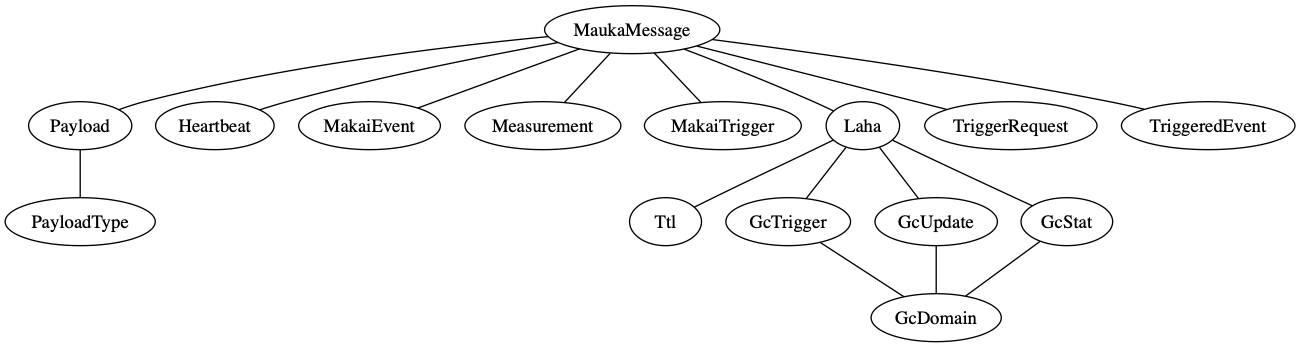
\includegraphics[width=\linewidth]{figures/mauka_messages.png}
	\caption{OPQ Mauka Communications Protocol Summary}
	\label{fig:mauka_messages}
\end{figure}

\subsubsection{Makai Communications Protocol}

Most communications take place inside of Mauka, however there are several communications channels that occur from Mauka to Makai. These include requesting event ids, sending triggers, and sending Box data rate commands. The communications protocols for these actions are described in this section.

Requesting event ids from Makai's Event Id Service is performed over a REQ/REP ZMQ socket. Requests from the client should be an empty string. Replies from the host should be a string that only includes the event\_id.

The ``Command" message (Table~\ref{table:Command}) is the base message used for sending commands to Makai and subsequently OPQ Boxes.

\begin{table}[H]
	\centering
	\caption{Command}
	\begin{tabular}{|c|c|p{8cm}|}
		\hline
		Field & Type & Description  \\
		\hline
		seq & uint32 & The command sequence number \\
		\hline
		box\_id & int32 & The Box id this command references \\
		\hline
		timestamp\_ms & uint64 & The timestamp of this command \\
		\hline
		identity & str & The formatted identity for this command \\
		\hline
		command & oneof(GetInfoCommand, GetDataCommand, SetMeasurementRateCommand, SendCommandToPlugin) & Command variant \\
		\hline
	\end{tabular}
	\label{table:Command}
\end{table}

The ``GetDataCommand" message (Table~\ref{table:GetDataCommand}) is sent with a ``Command" message when Mauka wants to trigger Boxes for data.

\begin{table}[H]
	\centering
	\caption{GetDataCommand}
	\begin{tabular}{|c|c|p{8cm}|}
		\hline
		Field & Type & Description  \\
		\hline
		start\_ms & uint64 & The start timestamp of the data request. \\
		\hline
		end\_ms & uint64 & The end timestamp of the data request. \\
		\hline
		wait & bool & If set, the Box will wait to send data if timestamps are in the future. \\
		\hline
	\end{tabular}
	\label{table:GetDataCommand}
\end{table}

The ``SetMeasurementRateCommand" (Table~\ref{table:SetMeasurementRateCommand}) message is sent with a ``Command" message when Mauka wants to modify the measurement rate of OPQ Boxes.

\begin{table}[H]
	\centering
	\caption{SetMeasurementRateCommand}
	\begin{tabular}{|c|c|p{8cm}|}
		\hline
		Field & Type & Description  \\
		\hline
		measurement\_window\_cycles & uint32 & How many grid cycles to process per measurements. \\
		\hline
	\end{tabular}
	\label{table:SetMeasurementRateCommand}
\end{table}

\subsubsection{Plugin Manager}
Plugins within Mauka are managed using a ``Plugin Manager". The Plugin Manager is responsible for starting, loading, unloading, reloading, terminating, and general management of Mauka plugins at runtime.

The Plugin Manager provides a networked command line interface (CLI) which communicates with the Plugin Manager's ZeroMQ endpoint which is utilized for sending commands and receiving responses to and from the Plugin Manager from any networked device. The CLI uses synchronous request/reply semantics where the client requests a message to the Plugin Manager and the Plugin Manager responds with a response.

The plugin manager can also be used as a library from within Mauka itself accessing the same functionality that is provided by the networked CLI. This functionality is used to initialize the set of plugins that are set to start when Mauka first starts.

Table~\ref{table:PluginManager} commands can be issued from a networked CLI client to interact with the Plugin Manager.

It's important to note some distinctions between the commands. Loading a plugin means loading a plugin from disk into memory where unloading means removing the plugin from memory. Enabling a plugins means that the plugin is loaded and enabled for running. Disabling a plugin means that the plugin is still loaded, but not enabled for running. Starting a plugin means to start a new process for a loaded and enabled plugin where stopping a plugin means to stop a current process and return it to an enabled and loaded state. Killing a plugin uses the OS to send a SIGKILL signal to the process for when its misbehaving and not stopping cleanly on its own.

\begin{table}[H]
	\centering
	\caption{Plugin Manager CLI Reference}
	\begin{tabular}{|c|c|p{8cm}|}
		\hline
		Command & Arguments & Description \\
		\hline
		completions & & Returns a list of completions for auto-complete. \\
		\hline
		disable-plugin & Plugin name & Disables the named plugin. \\
		\hline
		enable-plugin & Plugin name & Enables the named plugin. \\
		\hline
		help & & Displays the help text. \\
		\hline
		kill-plugin & Plugin name & Kills the named plugin. \\
		\hline
		load-config & Configuration path & Reloads the configuration from file. \\
		\hline
		load-plugin & Plugin name & Loads (or reloads) a plugin from disk. \\
		\hline
		list-plugins & & Lists all loaded plugins. \\
		\hline
		start-plugin & Plugin name & Starts the named plugin. \\
		\hline
		stop-plugin & Plugin name & Stops the named plugin. \\
		\hline
		stop-all-plugins & & Stops all running plugins. \\
		\hline
		restart-plugin & & Restarts the named plugin. \\
		\hline
		unload-plugin & Plugin name & Unloads the named plugin. \\
		\hline
	\end{tabular}
	\label{table:PluginManager}
\end{table}

\subsubsection{Mauka Configuration}
Mauka is highly configurable and it loads various static and dynamic configurations. Static configurations, or configurations that are loaded when Mauka starts are provided by a JSON file (appendix~\ref{appendix:MaukaConfig}). Dynamic configurations related to TTL and garbage collection are stored in the MongoDB and are discussed in detail in section~\ref{sec:gc_plugin}.

\subsubsection{Mauka Data Models}
Mauka works directly with the following data models: Measurements, Trends, Events, BoxEvents, Incidents, and Phenomena. The data models for these collections are described in this sections.

The measurements collection contains instantaneous measurements produced by Makai. The data model for measurements is described in Table~\ref{table:Measurement}.

\begin{table}[H]
	\centering
	\caption{Measurement Data Model}
	\begin{tabular}{|c|c|p{8cm}|}
		\hline
		Field & Type & Description \\
		\hline
		box\_id & str & OPQBox id \\
		\hline
		timestamp\_ms & int & Timestamp of the measurement in milliseconds \\
		\hline
		expire\_at & int & The timestamp in seconds that this document should be garbage collected \\
		\hline
		frequency & float & The instantaneous frequency measurement in Hz \\
		\hline
		voltage & float & The instantaneous voltage measurement \\
		\hline
		thd & float & The instantaneous THD measurement as a percentage \\
		\hline
	\end{tabular}
	\label{table:Measurements}
\end{table}

The trends collection provides summary statistics of frequency, voltage, and THD over a configurable time window. The data model for the trends collection is given in Table~\ref{table:Trends}.

\begin{table}[H]
	\centering
	\caption{Trend Data Model}
	\begin{tabular}{|c|c|p{8cm}|}
		\hline
		Field & Type & Description \\
		\hline
		min\_(thd, frequency, voltage) & float & Minimum values for THD, frequency, and voltage \\
		\hline
		max\_(thd, frequency, voltage) & float & Maximum values for THD, frequency, and voltage \\
		\hline
		average\_(thd, frequency, voltage) & float & Mean values for THD, frequency, and voltage \\
		\hline
		box\_id & str & OPQBox id \\
		\hline
		timestamp\_ms & int & Timestamp of end of trend in milliseconds \\
		\hline
		location & str & Location slug from the location that this trend originated from \\
		\hline
		expire\_at & int & Timestamp in seconds that this document should expire after \\
		\hline
	\end{tabular}
	\label{table:Trends}
\end{table}

The events collection contains metadata that map a Makai triggered event to a list of box\_events which points to raw data for each Box that was requested raw data for that event. The event data model is described in Table~\ref{table:Events}.

\begin{table}[H]
	\centering
	\caption{Event Data Model}
	\begin{tabular}{|c|c|p{8cm}|}
		\hline
		Field & Type & Description \\
		\hline
		event\_id & int & Id of the event generated \\
		\hline
		description & str & Description of the event \\
		\hline
		boxes\_triggered & [str] & A list of box\_ids that were triggered from this event \\
		\hline
		boxes\_received & [str] & A list of box\_ids that data was received from \\
		\hline
		target\_event\_start\_timestamp\_ms & int & Start of event \\
		\hline
		target\_event\_end\_timestamp\_ms & int & End of the event \\
		\hline
		expire\_at & int & Timestamp that this document should expire after \\
		\hline
	\end{tabular}
	\label{table:Events}
\end{table}

The box\_events data model is described in Table~\ref{table:BoxEvents}.

\begin{table}[H]
	\centering
	\caption{BoxEvent Data Model}
	\begin{tabular}{|c|c|p{8cm}|}
		\hline
		Field & Type & Description \\
		\hline
		event\_id & int & ID of the event this box\_event refers to \\
		\hline
		box\_id & str & ID of the OPQBox that sent data for this event \\
		\hline
		event\_start\_timestamp\_ms & int & Timestamp of the start of the event for this Box \\
		\hline
		event\_end\_timestamp\_ms & int & Timestamp of the end of the event for this Box \\
		\hline
		data\_fs\_filename & str & Reference to the waveform stored in gridfs \\
		\hline
		location & str & Location slug of where this Box sent data from \\
		\hline
	\end{tabular}
	\label{table:BoxEvents}
\end{table}

The Incidents collection keeps track of Incidents as defined by Laha. This collections includes metadata for classification and other contextual information relating to power incident. The Incident collection data model is described in Table~\ref{table:Incidents}.

\begin{table}[H]
	\centering
	\caption{Incident Data Model}
	\begin{tabular}{|c|c|p{8cm}|}
		\hline
		Field & Type & Description \\
		\hline
		incident\_id & int & ID of the incident \\
		\hline
		event\_id & int & ID of the event this incident references \\
		\hline
		box\_id & str & ID of the OPQBox that this incident references \\
		\hline
		start\_timestamp\_ms & int & Start of this incident \\
		\hline
		end\_timestamp\_ms & int & End of this incident \\
		\hline
		location & str & Location slug of where this incident originated from \\
		\hline
		measurement\_type & str & A description of the measurements used in this incident \\
		\hline
		deviation\_from\_nominal & float & The maximum deviation from nominal for the provided measurement\_type \\
		\hline
		measurements & [Measurement] & List of measurements stored in this incident \\
		\hline
		gridfs\_filename & str & Location in gridfs that the waveform for this incident is stored \\
		\hline
		ieee\_duration & str & An IEEE1159 duration \\
		\hline
		annotations & [str] & A list of annotations added to this incident \\
		\hline
		metadata & object & Metadata associated with this incident \\
		\hline
		expire\_at & int & This incident should expire after this timestamp \\
		\hline
	\end{tabular}
	\label{table:Incidents}
\end{table}

The ``ground\_truth" stores samples collected from the UH installed power meters. This collection is used to compare measurements and trends from OPQ Boxes to the ground truth measured by the UH meters. Each ground truth document consists of meter name, the feature stored, and descriptive statistics for that feature. The ``ground\_truth" data model is described in Table~\ref{table:ground_truth}.

\begin{table}[H]
	\centering
	\caption{Ground Truth Data Model}
	\begin{tabular}{|c|c|p{8cm}|}
		\hline
		Field & Type & Description \\
		\hline
		meter-name & str & Name of the meter this sample is from. \\
		\hline
		sample-type & str & Name of the feature present in this sample. \\
		\hline
		ts-s & int & The timestamp of this sample in seconds. \\
		\hline
		min & float & The minimum value of this feature over the time window. \\
		\hline
		max & float & The maximum value of this feature over the time window. \\
		\hline
		avg & float & The average value of this feature over the time window. \\
		\hline
		stddev & float & The standard deviation of values over the time window. \\
		\hline
	\end{tabular}
	\label{table:ground_truth}
\end{table}

The ``laha\_config" collection contains dynamic configuration options that Phenomena can alter. The collection is mainly used for defining the default TTL of collections that Mauka manages. The ``laha\_config" data model is described in Table~\ref{table:laha_config}.

\begin{table}[H]
	\centering
	\caption{Laha Config Data Model}
	\begin{tabular}{|c|c|p{8cm}|}
		\hline
		Field & Type & Description \\
		\hline
		box\_samples & int & Default TTL of Box samples. \\
		\hline
		measurements & int & Default TTL measurements. \\
		\hline
		trends & int & Default TTL trends. \\
		\hline
		events & int & Default TTL events and box\_events. \\
		\hline
		incidents & int & Default TTL incidents. \\
		\hline
	\end{tabular}
	\label{table:laha_config}
\end{table}

The ``laha\_stats" collection contains system statistics that measure various performance metrics in relation to Laha's optimizations. The full details of the ``laha\_stats" collection is provided in the section describing the ``SystemStatsPlugin"~\ref{lbl:SystemStatsPlugin}.

The ``makai\_config" collection contains default and Box override thresholds used by Makai's threshold triggering plugin. These items can be dynamically modified by the ``ThresholdOptimizationPlugin"\ref{subsubsec:threshold-optimization-pugin}.

\begin{table}[H]
	\centering
	\caption{Makai Config Data Model}
	\begin{tabular}{|c|c|p{8cm}|}
		\hline
		Field & Type & Description \\
		\hline
		default\_ref\_f & f64 & Default reference frequency \\
		\hline
		default\_ref\_v & f64 & Default reference voltage \\
		\hline
		default\_threshold\_percent\_f\_low & f64 & Default frequency percent low threshold \\
		\hline
		default\_threshold\_percent\_f\_high & f64 & Default frequency percent high threshold \\
		\hline
		default\_threshold\_percent\_v\_low & f64 & Default voltage percent low threshold \\
		\hline
		default\_threshold\_percent\_v\_high & f64 & Default voltage percent high threshold \\
		\hline
		default\_threshold\_percent\_thd\_high & f64 & Default THD percent high threshold \\
		\hline
		triggering\_overrides & [Makai Config Override] & List of Box specific overrides \\
		\hline
	\end{tabular}
	\label{table:makai_config}
\end{table}

\begin{table}[H]
	\centering
	\caption{Makai Config Override Data Model}
	\begin{tabular}{|c|c|p{8cm}|}
		\hline
		Field & Type & Description \\
		\hline
		box\_id & str & Override Box id \\
		\hline
		ref\_f & f64 & Override reference frequency \\
		\hline
		ref\_v & f64 & Override reference voltage \\
		\hline
		threshold\_percent\_f\_low & f64 & Override frequency percent low threshold \\
		\hline
		threshold\_percent\_f\_high & f64 & Override frequency percent high threshold \\
		\hline
		threshold\_percent\_v\_low & f64 & Override voltage percent low threshold \\
		\hline
		threshold\_percent\_v\_high & f64 & Override voltage percent high threshold \\
		\hline
		threshold\_percent\_thd\_high & f64 & Override THD percent high threshold \\
		\hline
	\end{tabular}
	\label{table:makai_config_override}
\end{table}

The ``phenomena" collection contains metadata relating to Phenomena produced by Mauka.

TODO

\subsubsection{PQ Plugins}
Mauka's functionality is provided by plugins that perform analysis, data management, health, and system tuning. Communication within Mauka is performed using type safe message passing. This section describes in detail how each plugin functions and also documents each plugins inputs and outputs.

\paragraph{BasePlugin}
All plugins derive from a single ``BasePlugin". The BasePlugin provides primitives for running plugins as separate processes, serialization and deserialization of type safe messages, communication over ZeroMQ, metrics collection, MongoDB communication, debugging, and plugin health.

To support running plugins as separate processes, the BasePlugin provides a ``run\_plugin" method that instantiates the new plugin inside of a new process. The BasePlugin provides signal handlers to catch SIGKILL and SIGINT signals from the system and cleanly exit the plugin process. The BasePlugin also contains an ``exit\_event" which can be set from other processes to inform the plugin to exit cleanly. This is used when Mauka is cleanly shutdown or when a plugin is stopped from the PluginManager.

When a BasePlugin process is started, the plugin creates a timer that runs at a configurable interval. When the timer fires, a heartbeat for the subclassing plugin is produced. This provides health information for each plugin within Mauka.

The BasePlugin provides automatic serialization and deserialization of protobuf Mauka messages produced and received for each plugin.

The BasePlugin provides functionality for automatically serializing and deserializing waveform from MongoDB's gridfs.

The BasePlugin provides ZMQ endpoints for producing and consuming messages to and from topics for each plugin. The BasePlugin ensures that all accesses to brokers are handled atomically with multiprocessing locks.

The BasePlugin keeps track of the number of messages sent and received for each plugin as well as the number of bytes sent and received for each plugin. This information is included in each plugin's heartbeat and later uses for calculating and storing metrics for each plugin.

The BasePlugin uses the configurable debugging interface to selective display debug messages for a plugin. Debug messages are only displayed for plugins that are configured to display debug messages in Mauka's configuration.

The BasePlugin provides a MongoDB client for each plugin for reading and writing to the database.

\paragraph{MakaiEventPlugin} The ``MakaiEventPlugin" is responsible for reading events newly created by Makai into Mauka. It performs feature extraction on the raw event data streams and forwards those features (or the raw data) to subscribing plugins. This allows Mauka to perform the important feature extraction once, and reuse those features in multiple plugins.

The MakaiEventPlugin subscribes to messages from the topic ``MakaiEventMessage". These messages are described in Table~\ref{table:MakaiEvent}. When a message is received, the plugin waits a configurable amount of time to ensure that Makai has finished writing data to the database. Once the data is in the database, the plugin loads the raw data and performs feature extraction.

The raw waveform from the OPQBox is serialized into a Payload (Table~\ref{table:Payload}) with PayloadType (Table~\ref{table:PayloadType}) ``ADC\_SAMPLES" and produced to the topic ``AdcSamples".

The raw Voltage is calculated by dividing each sample of the raw waveform by the calibration constant loaded from the database that is set for each device. The raw Voltage  is serialized into a Payload (Table~\ref{table:Payload}) with PayloadType (Table~\ref{table:PayloadType}) ``VOLTAGE\_RAW" and produced to the topic ``RawVoltage".

$V_{rms}$ is the peak-to-peak voltage over a configurable time window. By default, Mauka uses a time window of one electrical cycle at 60$Hz$ which works out to be $1/60$ seconds. $V_{rms}$ is calculated by moving a running window over the raw voltage waveform. The computation of $V_{rms}$ for each window with $n$ samples is given by equation~\ref{equation:Vrms}. The RMS Voltage  is serialized into a Payload (Table~\ref{table:Payload}) with PayloadType (Table~\ref{table:PayloadType}) ``VOLTAGE\_RMS\_WINDOWED" and produced to the topic ``RmsWindowedVoltage".

\begin{equation}
\label{equation:Vrms}
	V_{RMS} = \sqrt{\frac{\sum_{i=0}^{n} n_{i}^2}{n}}
\end{equation}

Windowed frequency is the frequency calculated for a configurable time window. By default, Mauka uses a time window of one electrical cycle at 60$Hz$ which works out to be $1/60$ seconds. The frequency is calculated by first smoothing the raw Voltage waveform by applying a $4^{th}$ order Butterworth filter to the waveform with a cutoff frequency of 500$Hz$ and a down sampling rate of 2. Then, a window is moved across the smoothed signal and the frequency is calculated for each window by performing a least squares regression and fitting a sinusoide. The windowed frequency is serialized into a Payload (Table~\ref{table:Payload}) with PayloadType (Table~\ref{table:PayloadType}) ``FREQUENCY\_WINDOWED" and produced to the topic ``WindowedFrequency".

When new events are received by the MakaiEventPlugin, a GcUpdate (Table~\ref{table:GcUpdate}) message is produced informing the LahaGcPlugin that all ``measurements" and ``trends" stored by Makai should receive a TTL of the newly created event.

\paragraph{FrequencyVariationPlugin}
The ``FrequencyVariationPlugin" is used to classify generic frequency sags, swells, and interruptions as defined by the IEEE1159 standard\cite{IEEE:2018:1159D3}. The plugin subscribes to messages from the ``WindowedFrequency" topic which includes a payload of frequency features over one electrical cycle.

When a message is received, the plugin uses configurable thresholds to find frequency fluctuations within the windowed frequency streams. The plugin is able to classify frequency swells, frequency interruptions, and frequency sags. When a new frequency variation is detected, a frequency incident is created and a GC\_UPDATE message is sent to the LahaGcPlugin to update the TTL of all measurements, trends, and events that belong to this new incident.

\paragraph{IEEE1159VoltagePlugin}
The ``IEEE1159VoltagePlugin" is a plugin that is able to classify voltage incidents in accordance to the IEEE1159 standard\cite{IEEE:2018:1159D3}. The plugin subscribes to messages from the ``RmsWindowedVoltage" topic which includes payloads of $V_{RMS}$ features over a window of one electrical cycle.

This plugin is capable of classifying voltage sags, swells, and interruptions as defined by the standard. The plugin works by identifying sags, swells, and interruptions and determining the duration of those events. If the duration or delta is large enough, a voltage incident is created and a GC\_UPDATE message is sent to the LahaGcPlugin asking it to update the TTL for all measurements, trends, and events that belong to this new incident.

\paragraph{ITICPlugin}
The ``ITICPlugin" analyzes $V_{rms}$ to determine where it falls within the ITIC curve\cite{thallam2000power}. The ITIC curve is a power acceptability curve that plots time on the x-axis and $V_{rms}$ on the y-axis. The ITIC curve is displayed in Figure~\ref{fig:IticCurve}.

\begin{figure}
	\centering
	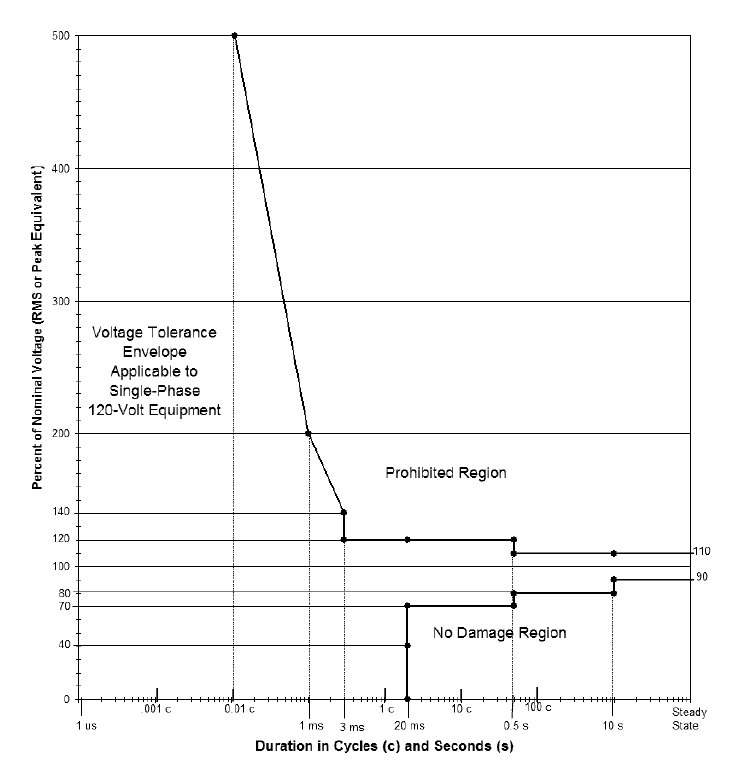
\includegraphics[width=\linewidth]{figures/itic.png}
	\caption{ITIC Curve}
	\label{fig:IticCurve}
\end{figure}

The purpose of the curve is to provide a tolerance envelope for single-phase 120V equipment. Meaning it defines the sustained Voltage tolerance at different time durations. The curve defines three regions. The first region is ``No Interruption" and generally includes all voltages with very short sustained durations. All power events within this region have no noticeable effect on power equipment. The second region, the ``No Damage Region", occurs during voltage sags for extended periods of time. Power events in this region may cause equipment interruptions, but it won't damage the equipment. The final region, the``Prohibited Region", is caused by sustained voltage swells and may cause damage to power equipment.

The ITICPlugin subscribes to the ``RmsWindowedVoltage" topic. When it receives a message, it extracts the windowed voltage features and uses a segmentation algorithm to split the features into segments of sustained voltage. The segmentation algorithm is rather naive and described below.

Given an array of values $A$, the length of the array $len(A)$, and a segmentation threshold $t$:
\begin{enumerate}
	\item Find all $i$ where $A_i - A_{i-1} > t$
	\item Segments over $A$, ($SA$), are then defined as [$SA_{0..i_0}, SA_{i_0..i_1}, \dots, SA_{i_n..len(A)}$]
\end{enumerate}

Once the segments are defined, we calculate the duration of each segment. We know that each sample in the $V_{rms}$ features represents one electrical cycle at 60$Hz$. Thus, to find the duration of a segment in milliseconds we can simply divide the number of cycles by the number of cycles in milliseconds. Thus, $duration\_ms = \frac{cycles}{0.06}$. The plugin also calculates the mean $V_{rms}$ for each segment. Once we have a duration and mean $V_{rms}$ for each segment, we can plot it on the ITIC curve and get a region classification.

In order to plot the value on the curve, the curve is first constructed as a set of polygons representing each ITIC region. Each polygon is represented by an array of points (see appendix~\ref{appendix:Itic}). Once the polygons are constructed, matplotlib's point-in-polygon algorithm is used to determine which ITIC region a point of $(duration\_ms, V_{rms})$ falls within. If a region of ``No Interruption" or "Prohibited" is returned, then a new ITIC incident is created and stored to the database.

If a new incident is created, a message is sent to the LahaGcPlugin informing the plugin to update the TTL of all measurements, trends, and events that belong to the incident.

\paragraph{LahaGcPlugin}\label{sec:gc_plugin}
Mauka provides custom garbage collection (GC) for identifying and removing ``uninteresting" data. This fulfills one of Laha's claims that it is able to manage data storage pressure while increasing the signal-to-noise ratio within the data set.

In order for Mauka to know when items should be GCed, all elements stored in the database are assigned a TTL. A default TTL is assigned when the element is first created, but can be updated later by Mauka plugins depending on if that data is deemed ``interesting".

Data within Laha is continually refined with context and by importance in Laha and by extension, OPQ does the same. As data is deemed interesting by Mauka, it is moved upward through the Laha hierarchy by Laha Actors. In the case of Mauka, this means moving raw data and features from OPQ Boxes into Mauka. When Mauka identifies interesting features of this data, it is moved into events. Interesting enough events are moved into Incidents, and collections of Incidents are moved into Phenomena. Whenever data is moved upwards, that data receives the TTL of its parent, and thus, will live for as long as its parent does.

Originally, Mauka relied on MongoDB's Time-to-Live (TTL) semantics for expiring and deleting uninteresting data. This did not provide the flexibility needed for Mauka's refined garbage collection needs. For example, MongoDB's TTL could only be applied to entire collections and not dynamically to individual elements in the collection. MongoDB's TTL was also difficult to update dynamically based on the state of the system. Because we want to assign TTLs dynamically (as interesting data is moved upwards) we required a more robust solution to TTL and GC management.

Default TTLs are dynamically stored in the Mongo database under the ``laha\_config" collection and the ``ttls" key. Since the TTLs are stored in the database, they can be updated and tuned by Mauka's Phenomena.

Table~\ref{table:DefaultTtls} displays the default TTL in seconds for each OPQ collection.

\begin{table}[H]
	\centering
	\caption{Default TTLs for OPQ Collections}
	\begin{tabular}{|c|c|}
		\hline
		Collection & Default TTL (seconds) \\
		\hline
		box\_samples & 900 \\
		\hline
		measurements & 86400 \\
		\hline
		trends & 604800 \\
		\hline
		events & 2592000 \\
		\hline
		incidents & 31536000 \\
		\hline
		phenomena & Does not expire \\
		\hline
	\end{tabular}
	\label{table:DefaultTtls}
\end{table}

As each item is saved to the database, it is assigned with a default TTL as described in Table~\ref{table:DefaultTtls}. If the item that was assigned to the database is later deemed important by Mauka and is referenced by a parent item, it receives the TTL of the parent item allowing that data to live as long as the parent does. If the parent item is a Phenomena, then all data relating to that Phenomena (from all levels are the hierarchy) will live forever. The process of updating

The Mauka plugin ``LahaGcPlugin" is responsible for GC and TTL management. Each plugin in Mauka produces a heartbeat at a predefined interval. GC within the LahaGcPlugin takes place every time the plugin produces a heartbeat.

Other than heartbeats, it's also possible to trigger the GC by sending a message to the GC plugin with a list of collections that should be GC\@.

When the LahaGcPlugin receives a ``GcTrigger" message, it extracts from the message the list of collections that should be GCed. Heartbeats will trigger all collections to be GCed.

The measurements and trends collections perform GC by simply removing from the database all measurements and trends that have a TTL that is older than the current date and time.

Events in OPQ are spread out over three collections: events, box\_events, and gridfs files. Events contain metadata about an event which includes information about all Boxes that sent data in response to that event. Each Box that sent data for an event will spawn a box\_event document which includes information relating to a Box for a specific event. Further, each box\_event document points to where the raw data is stored in MongoDB using the gridfs data layer provided by the database.

In order to GC events, first all events with a TTL less than the current date and time are identified. From the events, we look up the corresponding box\_events. From each box\_event, we look up corresponding raw data in gridfs. First the gridfs data is removed, then the box\_events are removed, and finally the events themselves are removed.

To GC incidents, a similar algorithm is provided. First, incidents with a TTL less than the current date and time are identified. From these identified incidents, Mauka looks up and removes the corresponding data in gridfs. Finally, the incidents are removed.

Phenomena, being the top of the hierarchy are GCed the least since it provides the most context for optimizing the DSN. Phenomena are only GCed when they are shown to be incorrect or are otherwise unused over the period of a year. Thus, Phenomena take the same default TTL as Incidents. Phenomena differ from Incidents in that every time a Phenomena is referenced by the DSN, it's TTL is renewed for another year from the last use date. Similarly to other collections, when a Phenomena's TTL is updated, all collections that the Phenomena references will also have their TTL updated.

Metrics for GC (i.e.\ the number of items removed per collection) are stored providing insights to data management and effectiveness.

The Mauka GC plugin does not manage raw data on OPQ Boxes. Instead, OPQ Boxes manage their own internal data buffer with a TTL that can be configured on the Box.

Dynamically updating TTLs is also performed by the LahaGcPlugin. The LahaGcPlugin listens for specific ``Ttl" messages that contain the source item that the TTL is being updated for. Then all child elements of the source element also have their TTLs updated. TTLs are updated in the following manner.

When new events are created, the TTL of measurements and trends that coincide with that event receive the TTL of the event. When incidents are created, the events, trends, and measurements associated with that incident receive the TTL of the incident. When Phenomena are created, the TTLs of incidents, events, trends, and measurements are assigned the TTL of the Phenomena (which is infinite).

\paragraph{MockPlugin}
The ``MockPlugin" is a special plugin that can be instantiated at run time and sends and receives messages to configurable topics. This plugin is useful for debugging and rerunning (or running new) analysis over old data. As an example, let's say a new plugin Foo is designed. We want to run historical data through Foo. To do that, the MockPlugin can be configured to read the database for all old events, and then construct a message to Foo so that Foo runs its analysis over those events.

\paragraph{OutagePlugin}
The ``OutagePlugin" classifies power outages. Since no real power data is produced during an outage, this plugin only subscribes to its own heartbeats. When a heartbeat is received, the outage plugin looks up in the database all OPQBoxes that are marked ``down" by OPQHealth and not marked as ``unplugged" in the database. This plugin keeps track of current outages so that if an OPQBox is already in an outage state a new outage Incident is not created on each subsequent heartbeat.

When outage incidents are created, TTL update messages are not sent because there is no data during the time period of an outage to adjust the TTL for.

\paragraph{PrintPlugin}
The ``PrintPlugin" is a special plugin that is mainly used for debugging. It subscribes to all topics and simply prints the contents of the message to STDOUT. This is useful in development or when bringing up a new Mauka system to ensure that the communications infrastructure is in place. It can also be enabled at runtime from the Mauka CLI to debug all communication channels for all plugins.

\paragraph{SemiF47Plugin}
The ``SemiF47" plugin is another plugin like the IticPlugin that plots voltage and duration against a power acceptability curve. In this case, the standard used is the SemiF47 standard\cite{semif47}. Rather than using a point-in-polygon approach, this plugin reads the $V_{RMS}$ features sequentially and uses a state machine to keep track of the current classification. This plugin only classifies values as a ``violation" or as ``nominal".

The SemiF47 curve is displayed in Figure~\ref{fig:SemiF47Curve}.

\begin{figure}
	\centering
	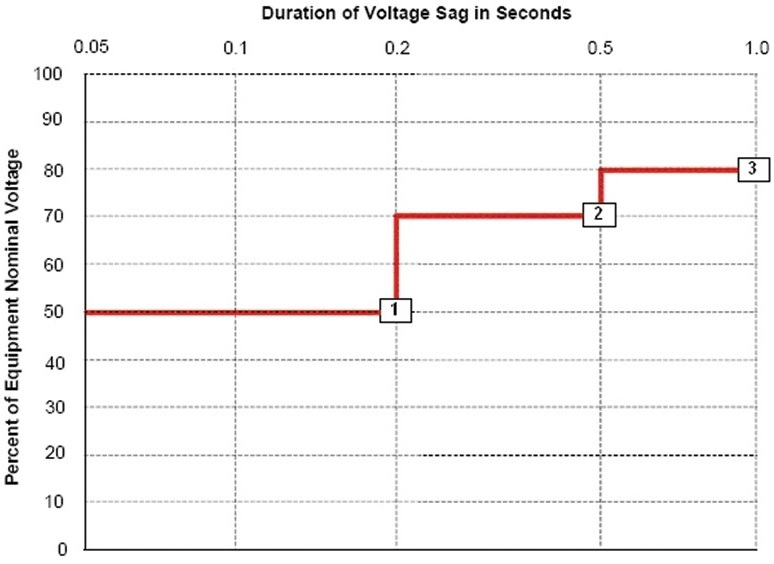
\includegraphics[width=0.6\linewidth]{figures/semif47.jpg}
	\caption{SemiF47 Curve}
	\label{fig:SemiF47Curve}
\end{figure}

SemiF47 is described in Table~\ref{fig:SemiF47Table}.

\begin{figure}
	\centering
	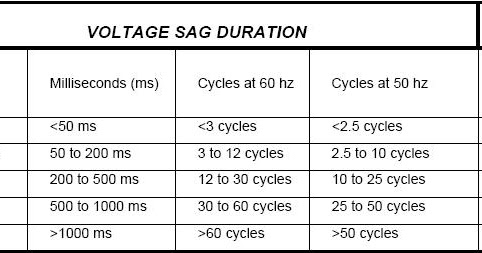
\includegraphics[width=0.6\linewidth]{figures/semif47_table.jpg}
	\caption{SemiF47 Table}
	\label{fig:SemiF47Table}
\end{figure}


\paragraph{StatusPlugin}
Mauka provides a health endpoint that can be queried by OPQ Health to determine the health status of Mauka. The health status is saved to a database by Health and shown in OPQ View.

The Mauka plugin ``StatusPlugin" is responsible for obtaining and providing the status of the OPQ Mauka service. The plugin subscribes to heartbeats sent at configurable intervals from all other plugins including itself. When the plugin receives a heartbeat, it updates its internal state which includes a mapping of all plugins, their state, and the last time that plugin sent a heartbeat.

The plugin provides a configurable HTTP endpoint which is queried by OPQ Health. The plugin extracts the internal health state and serializes the state as JSON using the protocol described in Table~\ref{table:HealthProtocol}. This protocol is standardized for health collection across all OPQ services.

\begin{table}[H]
	\centering
	\caption{Mauka HealthProtocol}
	\begin{tabular}{|c|c|c|}
		\hline
		Field & Type & Description \\
		\hline
		name & string & Name of the service \\
		\hline
		ok & bool & Whether the entire service is ok or not \\
		\hline
		timestamp & int & The timestamp of when the health request was received \\
		\hline
		subcomponents & [HealthProtocol] & Health protocol for each plugin \\
		\hline
	\end{tabular}
	\label{table:HealthProtocol}
\end{table}

\paragraph{SystemStatsPlugin}\label{lbl:SystemStatsPlugin}
Mauka collects and stores many different types of performance metrics in order to demonstrate the efficacy of Laha as implemented in Mauka. The metrics are collected by the ``SystemStatsPlugin" Mauka plugin and are stored in the MongoDB collection `laha\_metrics`.

The metrics are conditioned and displayed in OPQ View for easy analysis. It's possible to select a start and end date/time to configure the time window of metrics displayed in view. Examples of Mauka's metrics displayed in OPQ View are shown in figures~\ref{fig:Metrics1},~\ref{fig:Metrics2}, and~\ref{fig:Metrics3}.

\begin{figure}
	\centering
	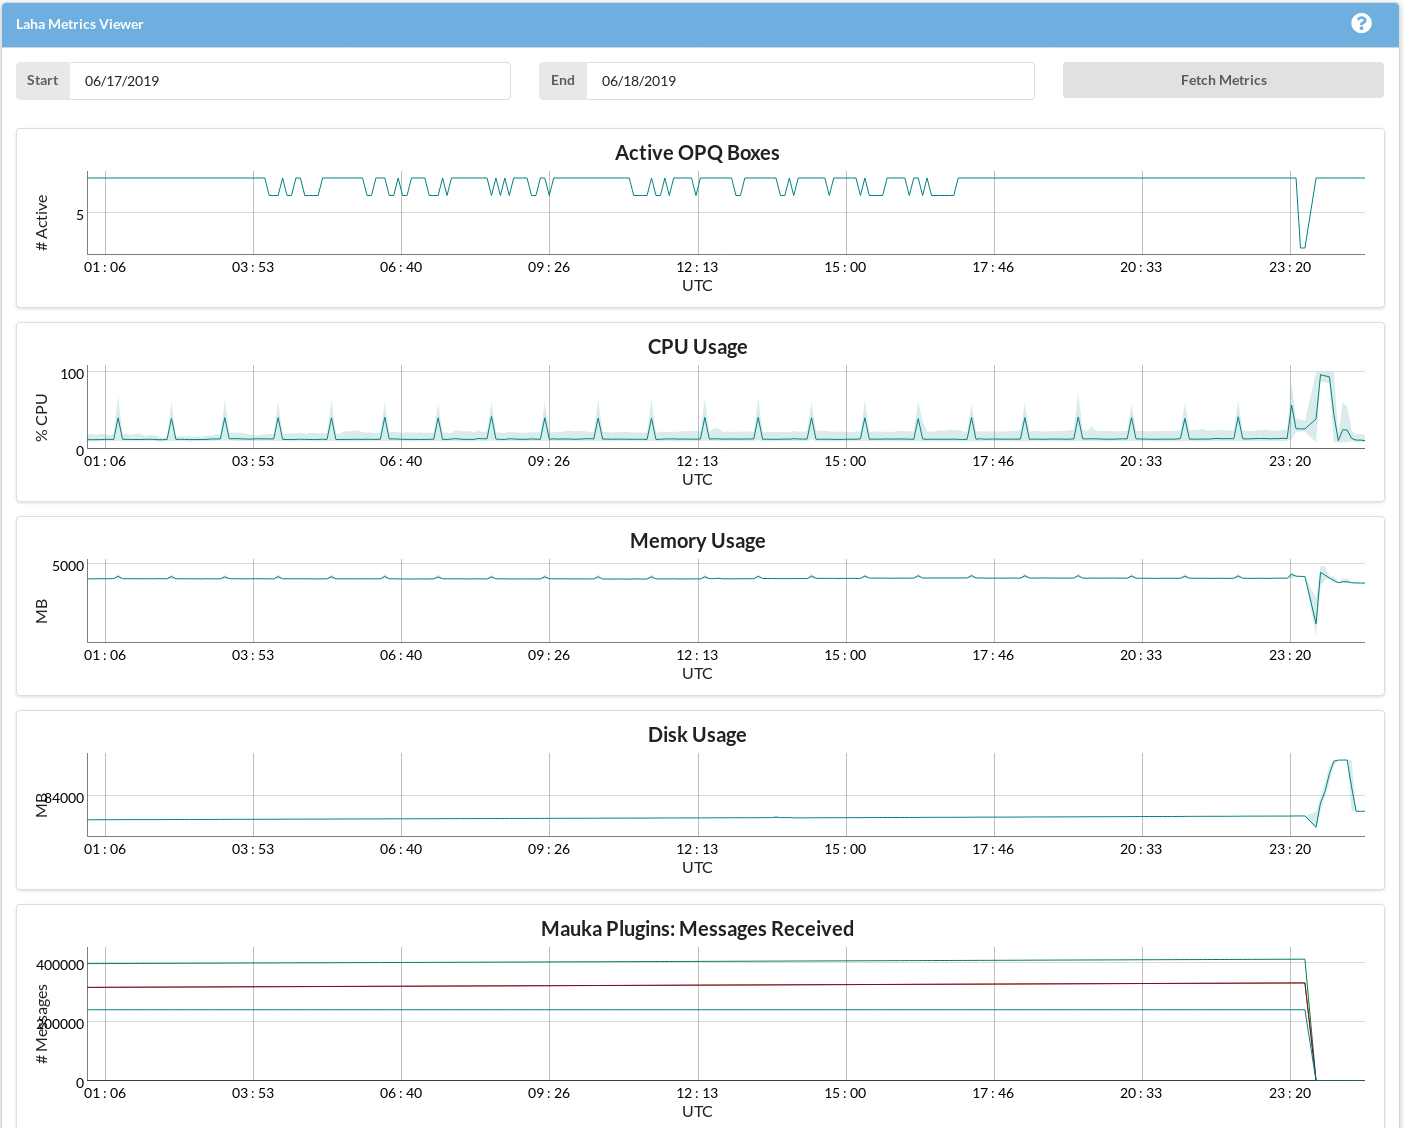
\includegraphics[width=\linewidth]{figures/metrics_1.png}
	\caption{OPQ Mauka Metrics I}
	\label{fig:Metrics1}
\end{figure}

\begin{figure}
	\centering
	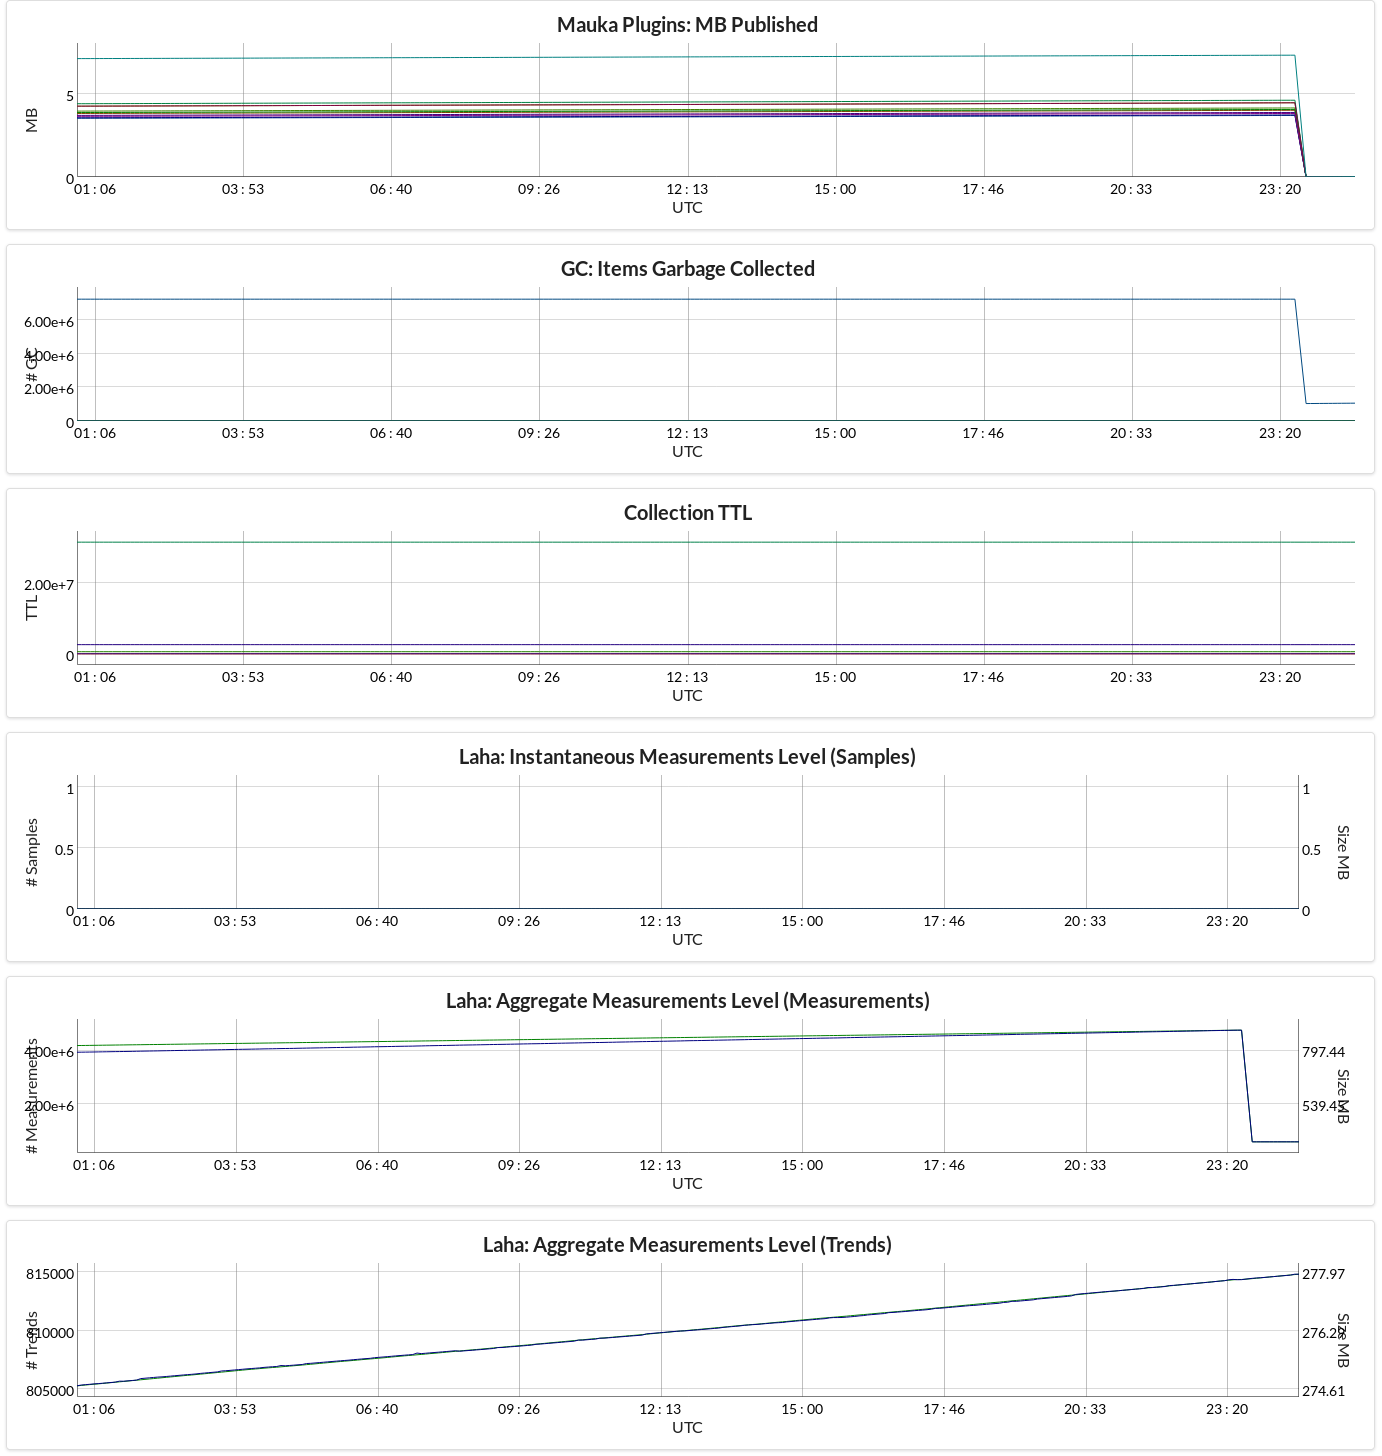
\includegraphics[width=\linewidth]{figures/metrics_2.png}
	\caption{OPQ Mauka Metrics II}
	\label{fig:Metrics2}
\end{figure}

\begin{figure}
	\centering
	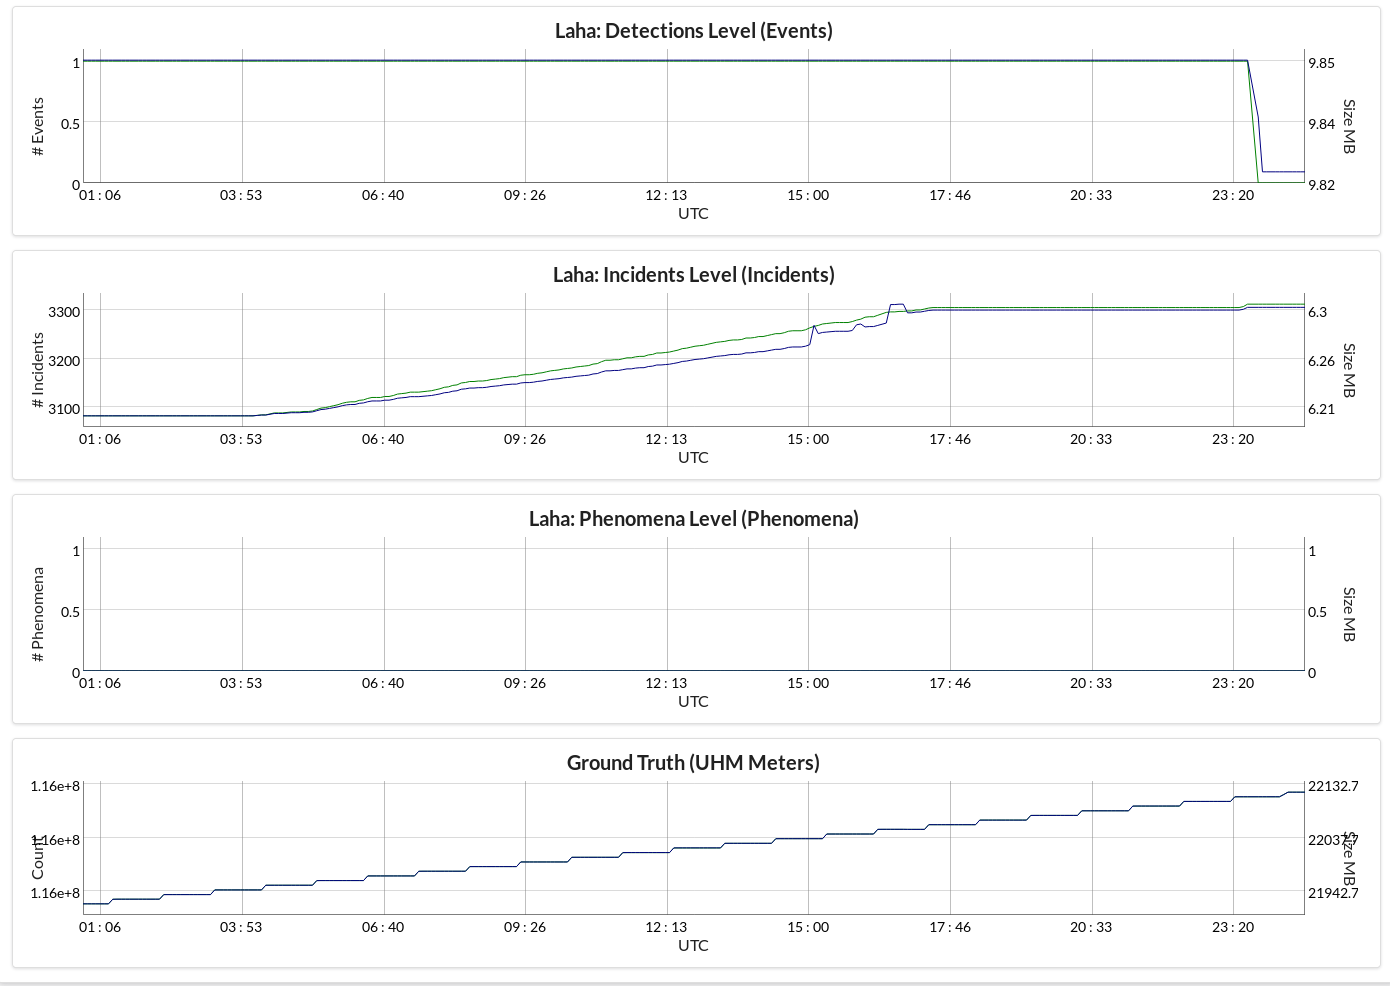
\includegraphics[width=\linewidth]{figures/metrics_3.png}
	\caption{OPQ Mauka Metrics III}
	\label{fig:Metrics3}
\end{figure}

The types of metrics collected include plugin statistics, system statistics, and Laha statistics which provide metrics on data usage and TTL for data stored within each Laha level as well as garbage collection statistics for each level of the hierarchy.

Metrics are collected at a configurable interval. System statistics such as CPU usage, memory usage, and disk usage are sampled once every 10 seconds. Once every 5 minutes, all metrics are saved to disk. The system statistic metrics which are sampled more frequency are rolled into a 5 minute metric only storing min, max, mean, variance, count, and start and end timestamp.

Mauka metrics consist of nested documents. The following Table swill describe each of the documents stored in the metrics collection.

The base document shown in Table~\ref{table:Metrics} contains links to all of the high level metrics that Mauka collects. This includes metrics for plugins, system statistics, Laha metrics, and ground truth.

\begin{table}[H]
	\centering
	\caption{Mauka Metrics}
	\begin{tabular}{|c|c|c|}
		\hline
		Metric & Type & Description \\
		plugin\_stats & [PluginStat] & List of metrics for each plugin. \\
		\hline
		system\_stats & [SystemStat] & System statistics for CPU, memory, and disk usage. \\
		\hline
		laha\_stats & [LahaStat] & Statistics on count, size, and TTL for each collection. \\
		\hline
		ground\_truth\_count & int & Count of ground truth documents. \\
		\hline
		ground\_truth\_size\_bytes & int & Size of ground truth in bytes. \\
		\hline
	\end{tabular}
	\label{table:Metrics}
\end{table}

Plugin metrics are described in Table~\ref{table:MetricsPluginStat} and mainly record the plugin name and the number and size of messages received and produced for each plugin.

\begin{table}[H]
	\centering
	\caption{PluginStat}
	\begin{tabular}{|c|c|c|}
		\hline
		Metric & Type & Description \\
		\hline
		messages\_received & int & The number of messages the plugin has received. \\
		\hline
		messages\_published & int & The number of messages the plugin has published. \\
		\hline
		bytes\_received & int & The number of bytes the plugin has received. \\
		\hline
		bytes\_published & int & The number of bytes the plugin has published. \\
		\hline
	\end{tabular}
	\label{table:MetricsPluginStat}
\end{table}

System metrics as shown in Table~\ref{table:MetricsSystemStat} use descriptive statistics over a time window to collect the minimum, maximum, mean, variance, and count of memory, disk, and CPU usage.

\begin{table}[H]
	\centering
	\caption{SystemStat}
	\begin{tabular}{|c|c|c|}
		\hline
		Metric & Type & Description \\
		\hline
		min & float & Minimum value over time window. \\
		\hline
		max & float & Maximum value over time window. \\
		\hline
		mean & float & Mean value over time window. \\
		\hline
		var & float & Variance of values over time window. \\
		\hline
		cnt & int & The number of items sampled over time window. \\
		\hline
		start\_timestamp\_s & int & Start timestamp of time window. \\
		\hline
		end\_timestamp\_s & int & End timestamp of time window. \\
		\hline
	\end{tabular}
	\label{table:MetricsSystemStat}
\end{table}

The Laha metrics described in Table~\ref{table:MetricsLaha} store metrics relating to the TTL, size, and count of Laha collections.

\begin{table}[H]
	\centering
	\caption{LahaStat}
	\begin{tabular}{|c|c|c|}
		\hline
		Metric & Type & Description \\
		\hline
		ttl & int & Default TTL for a Laha level. \\
		\hline
		count & int & Number of items in a Laha level. \\
		\hline
		size\_bytes & int & Size of a Laha level in bytes. \\
		\hline
	\end{tabular}
	\label{table:MetricsLaha}
\end{table}

\paragraph{ThdPlugin}
The ``ThdPlugin" classifies abnormal amounts of total harmonic distortion (THD) in a power waveform. THD is a measure of amount of noise in the frequency at multiples of 60Hz. The ThdPlugin subscribes to messages from the ``AdcSamples" topic which include payloads consisting of raw samples from the OPQBoxes. THD is calculated using a rolling window of one electrical cycle over the waveform. For each window, THD is calculated by equation~\ref{equation:Thd}.

\begin{equation}
\label{equation:Thd}
	THD_F = \frac{\sqrt{V_2^2 + V_3^2 + V_4^2 + \dots}}{V_1}
\end{equation}

For each continuous set of windows that has THD higher than the configured threshold, a THD Incident is created. If an Incident is created, this plugin sends a GC\_UPDATE message to the LahaGcPlugin informing it that it should update all measurements, trends, and events that belong to the new incident to match the incident's TTL\@.


\paragraph{TransientPlugin}
The ``TransientPlugin" is responsible for classifying frequency transients in power waveforms. The plugin subscribes to messages from the ``RawVoltage" topic which contains a calibrated power waveform payload. The TransientPlugin is capable of classifying impulsive, arcing, oscillatory, and periodic notching transients. A decision tree is utilized to select the most likely transient type and then further analysis is used to perform the actual classification of transients.

The full details of our transient classification system are published in the Proceedings of the Ninth International Conference on Smart Grids, Green Communications and IT Energy-aware Technologies\cite{csdl2-19-02}.

When a transient is classified a new transient Incident is created. If an incident is created, this plugin sends a GC\_UPDATE message to the LahaGcPlugin informing it to update the TTLs for all measurements, trends, and events that belong to this new incident.

\paragraph{TriggerPlugin}\label{sec:trigger_plugin}
The ``TriggerPlugin" provides Mauka with the functionality to trigger OPQ Boxes itself instead of relying on Makai for triggering. Generally, Mauka is only provided with event\_ids when Makai triggers Boxes based off of their low-fidelity data streams. Mauka then loads the associated event data from the database, performs cycle level feature extraction, and then forwards those features to analysis plugins for PQ analysis.

This plugin takes advantage of Phenomena in order to find incidents that may not have passed Makai's triggering thresholds.

This plugin consists of two threads running in a single process. The main thread (or the plugin thread) is responsible for listening for ``TriggerRequest" messages from other plugins and sending trigger requests to Makai's acquisition broker. The second data thread is responsible for listening for data from triggered Boxes routed through Makai.

The only stateful component between a data request and a data response is an identity string which is a specially crafted string that allows Makai to route requests through its services. The format of an identity string is ``[topic]\_[event\_token]\_[uuid]". In Mauka's case, the ``[topic]" is always set to ``mauka", the ``[event\_token]" is a randomly generated v4 UUID (which provides $2^{122}$ bits of collision space), and the ``[uuid]" is the box\_id of the Box being triggered. The issue however is that both threads need to know more than just the identity. For instance, they need to know things like which ``event\_id" and ``incident\_id" a data response belongs to to or which Boxes we are still waiting for a response from.

To accomplish data sharing between the two threads, a thread safe ``TriggerRecords" class was created. This class uses a reentrant lock to lock mappings from ``event\_token" to all of ``event\_id", ``incident\_id", ``timestamp\_ms" (of record insert), and ``triggered\_boxes".  Details of how these mappings are used will be provided in later paragraphs.

This plugin listens for ``TriggerRequest" messages from other plugins. When it receives a ``TriggerRequest", it constructs protobuf data commands that Makai can consume. Each data command is for a single Box and includes start and end timestamps as milliseconds since the epoch. Each data command also contains an identity string which determines how the message is routed through Makai's services.

The data commands\ref{table:Command} are serialized and sent over a ZMQ PUSH/PULL socket to Makai's acquisition broker. Makai's acquisition broker then goes out to the requested Boxes (if they are available) and requests raw data for the requested time window.

Previously, Makai handled all Event storage. With this plugin, Mauka now has to handle Event storage for Boxes that Mauka has triggered. This includes creating and modifying the Event document metadata, BoxEvent document metadata, and gridfs waveform storage.

Just after the data commands are sent to Makai's acquisition broker, a ZMQ REQ/REP channel is used to query Makai's event id service. Makai's event id service provides atomic access to the next available event id for storage of events in the Mongo database. Once the next available event id is received by Mauka, it is used to create a new Event document in the database with the new event id, the event time window, and a list of triggered Boxes.

Just after the event\_id is received, the plugin updates the thread-safe TriggerMappings class with mappings from the new event\_token to the new event\_id, the incident\_id, the Boxes triggered, and the timestamp of the triggers.

In order to receive data requested from the Boxes, this plugin starts a separate data thread when this plugin starts. The data thread connects to a Makai acquisition broker endpoint over ZMQ using a PUB/SUB channel. The data thread subscribes to all topics that start with ``mauka\_" which will match all identities generated by Mauka and will ignore trigger requests initiated by Makai.

When data is received for a Box in the data thread, the metadata and uncalibrated waveform cycles are extracted from the deserialized message. We also extract event\_id information from the thread-safe TriggerRecords class using the response's event\_token. A ``BoxEvent" document is created in the Mongo database for the newly received data and the waveform is written to gridfs and metadata pointing to the gridfs file is provided in the BoxEvent.

Next, the original Event document is updated to insert the received box\_id into the ``received\_boxes" field.

Then, the received Box id is removed from the TriggerRecords class since we are no longer waiting on it. If this was the last Box we were waiting on for an associated event, then the trigger record associated with this identity is removed and a message with the new event\_id is sent to the ``MakaiEventPlugin" which then forwards feature extracted data to the rest of the analysis pipeline.

By using the above approach, we ensure that we never request analysis of the data until all triggered Boxes are received for a particular event. However, we can run into the issue of triggered Boxes never returning data for a request. To deal with this issue, the TriggerRecords class timestamps each record that is inserted. If the data receive thread does not receive data from all triggered Boxes within a configurable amount of time (default 1 minute), then the records are removed and an event\_id is sent to the ``MakaiEventPlugin" so that it can process data for all of the Boxes that it did receive.

Data triggered from Mauka is fundamentally different than data triggered from Makai. That's because Boxes triggered from Mauka are always triggered from an associated Incident or Phenomena. If new Incidents are found from this data and they are similar to the original Incident that caused Mauka to trigger, then we have found a global event and possible Phenomena that would not have been observed using Makai's triggering alone. This requires extra semantic information to be passed to the ``MakaiEventPlugin" and other analysis plugins. Data received from Mauka triggers are always forwarded with the associated Incident or Phenomena id so that the relationships can be tracked and maintained.

\paragraph{ThresholdOptimizationPlugin}\label{subsubsec:threshold-optimization-pugin}
The ThresholdOptimizationPlugin is responsible for modifying dynamic triggering thresholds within Makai. Makai utilizes two methods for triggering Boxes. One method called ``Napali" was produced by Sergey Negrashov as part of his dissertation research. The Napali trigger uses a windowed statistical model for triggering devices based off of metric distance from standard deviations and means. The second approach to triggering is a threshold trigger which watches Frequency, Voltage, and THD levels to determine if they've passed certain thresholds. This plugin works with the second type of triggering, the threshold trigger. Threshold based triggering is described in section~\ref{subsubsec:dynamic-triggering}.

Thresholds are stored in MongoDB and consist of default thresholds and override thresholds which are thresholds set specifically for individual devices. This plugin can dynamically modify both types of thresholds. The data model for thresholds are presented in Table~\ref{table:makai_config}.

This plugin receives the MaukaMessage variant ``ThresholdOptimizationRequest"\ref{table:ThresholdOptimziationRequest}. When a request is received, the default thresholds can be updated, a single override threshold can be updated, or both can be updated at the same time.

For any default value in the request that is larger than 0, the default threshold value in the database is updated with the new request value. If the request contains an override value larger than 0, this plugin first checks to see an override for that Box already exists in the database. If an override already exists, then the override is updated with the new override values from the request. If the override does not exist, then a new override is created with default values and the override values are updated from the request.

\paragraph{RateOptimizationPlugin}

The ``RateOptimizationPlugin" is responsible for modifying the send rate of Measurements for specific Boxes. This plugin subscribes to ``RateOptimizationRequest" messages\ref{table:RateOptimizationRequest} which include a Box id and requested sample rate for the Measurements collection.

Requests from this plugin are sent from Phenomena when a Phenomena believes that changing the Measurement rate of a Box or Boxes could enhance Mauka's ability to discover signals of interest.

When a request is received, this plugin sends a Makai Command\ref{table:Command} to Makai's acquisition broker over a ZMQ socket. The command message includes the Box id and Measurement sample rate. Makai then handles forwarding the command to the relevant Box which will then change its Measurement rate to match that of the request.

\paragraph{TtlOptimizationPlugin}\label{subsubsec:ttl-optimization-pugin}

The ``TtlOptimizationPlugin" is responsible for dynamically modifying ``laha\_config" collection TTL values. This plugin subscribes to ``TtlOptimizationRequest" messages\ref{table:TtlOptimizationRequest}.

When a request is received, the corresponding TTL value in the database is updated to match the requested value.

This plugin only affects TTL values for newly generated Measurements, Trends, Event, Incidents, and Phenomena and will not update the TTL values of documents that are already in the database.

\subsubsection{Debugging OPQMauka}
The Mauka system can be configured so that only specified plugins print debug messages. This is accomplished by specifying the names of the plugins which should print debug output in Mauka's configuration file. Without this functionality, parsing through the entirety of Mauka's log output would be a daunting task.

\subsection{OPQ: View}\label{subsec:opq:-view}
OPQView is a web application that provides visualization, notification, and user management services for data, sensors, and user accounts with the OPQ framework. OPQView is built using Meteor.js and provides a Reactive view of the underlying data stored in the OPQ database.

A screenshot of OPQView in action is provided in Figure~\ref{fig:opq-view}.

\begin{figure}
	\centering
	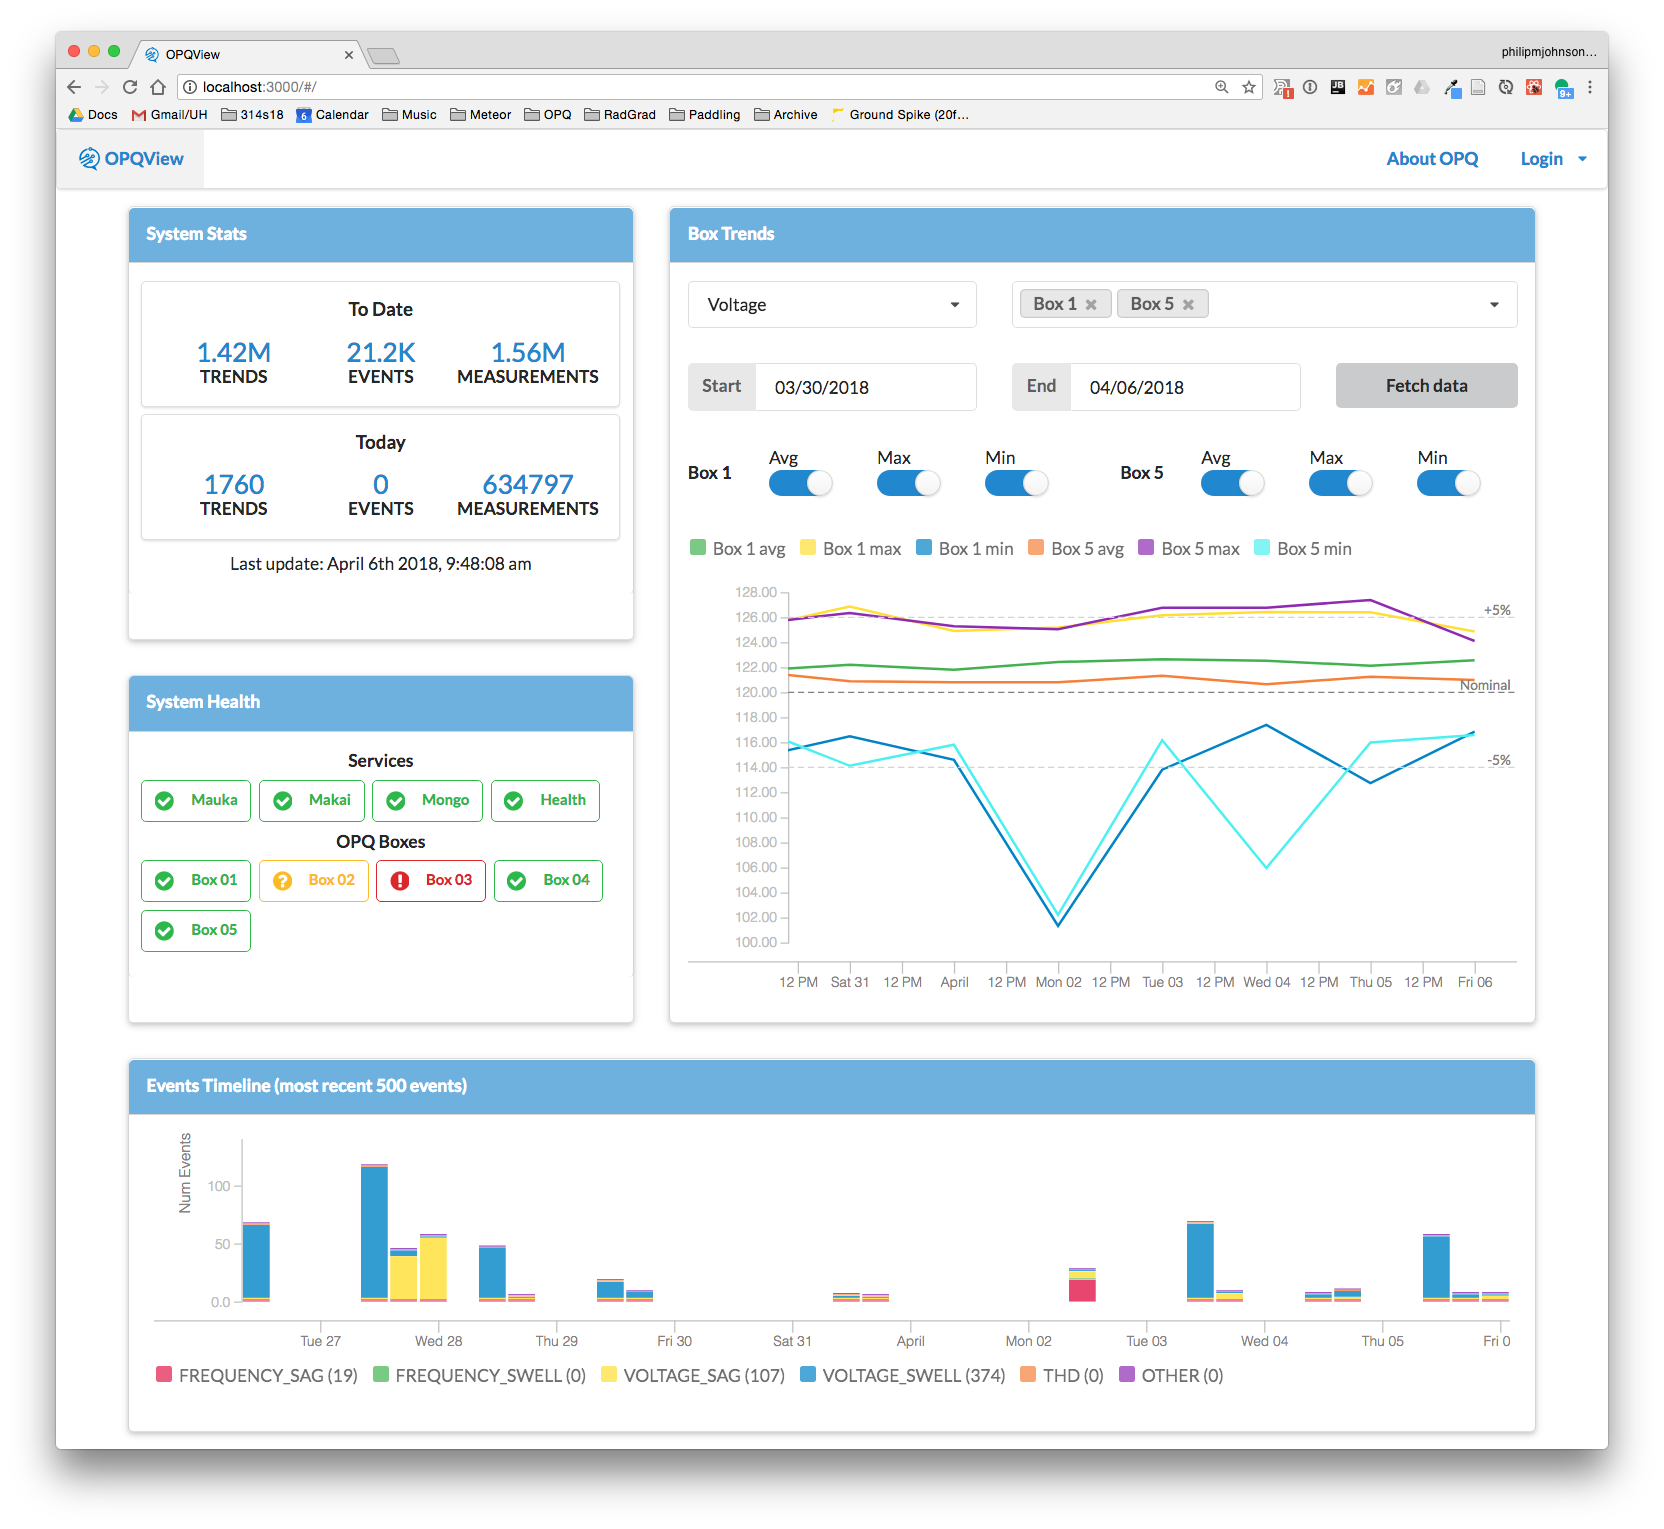
\includegraphics[width=1\linewidth]{figures/opqview-landing-page.png}
	\caption{OPQ View Screenshot}\label{fig:opq-view}
\end{figure}

For the most part, OPQ View serves as a client for displaying PQ information collected and analyzed by the rest of the framework. However, OPQ View provides two components that are directly related to this dissertation.

OPQ View provides the ability to manually define minimum and maximum triggering thresholds for Voltage, Frequency, and THD used by Makai. Figure~\ref{fig:view_thresholds} shows what this functionality looks like as implemented in View.

\begin{figure}
	\centering
	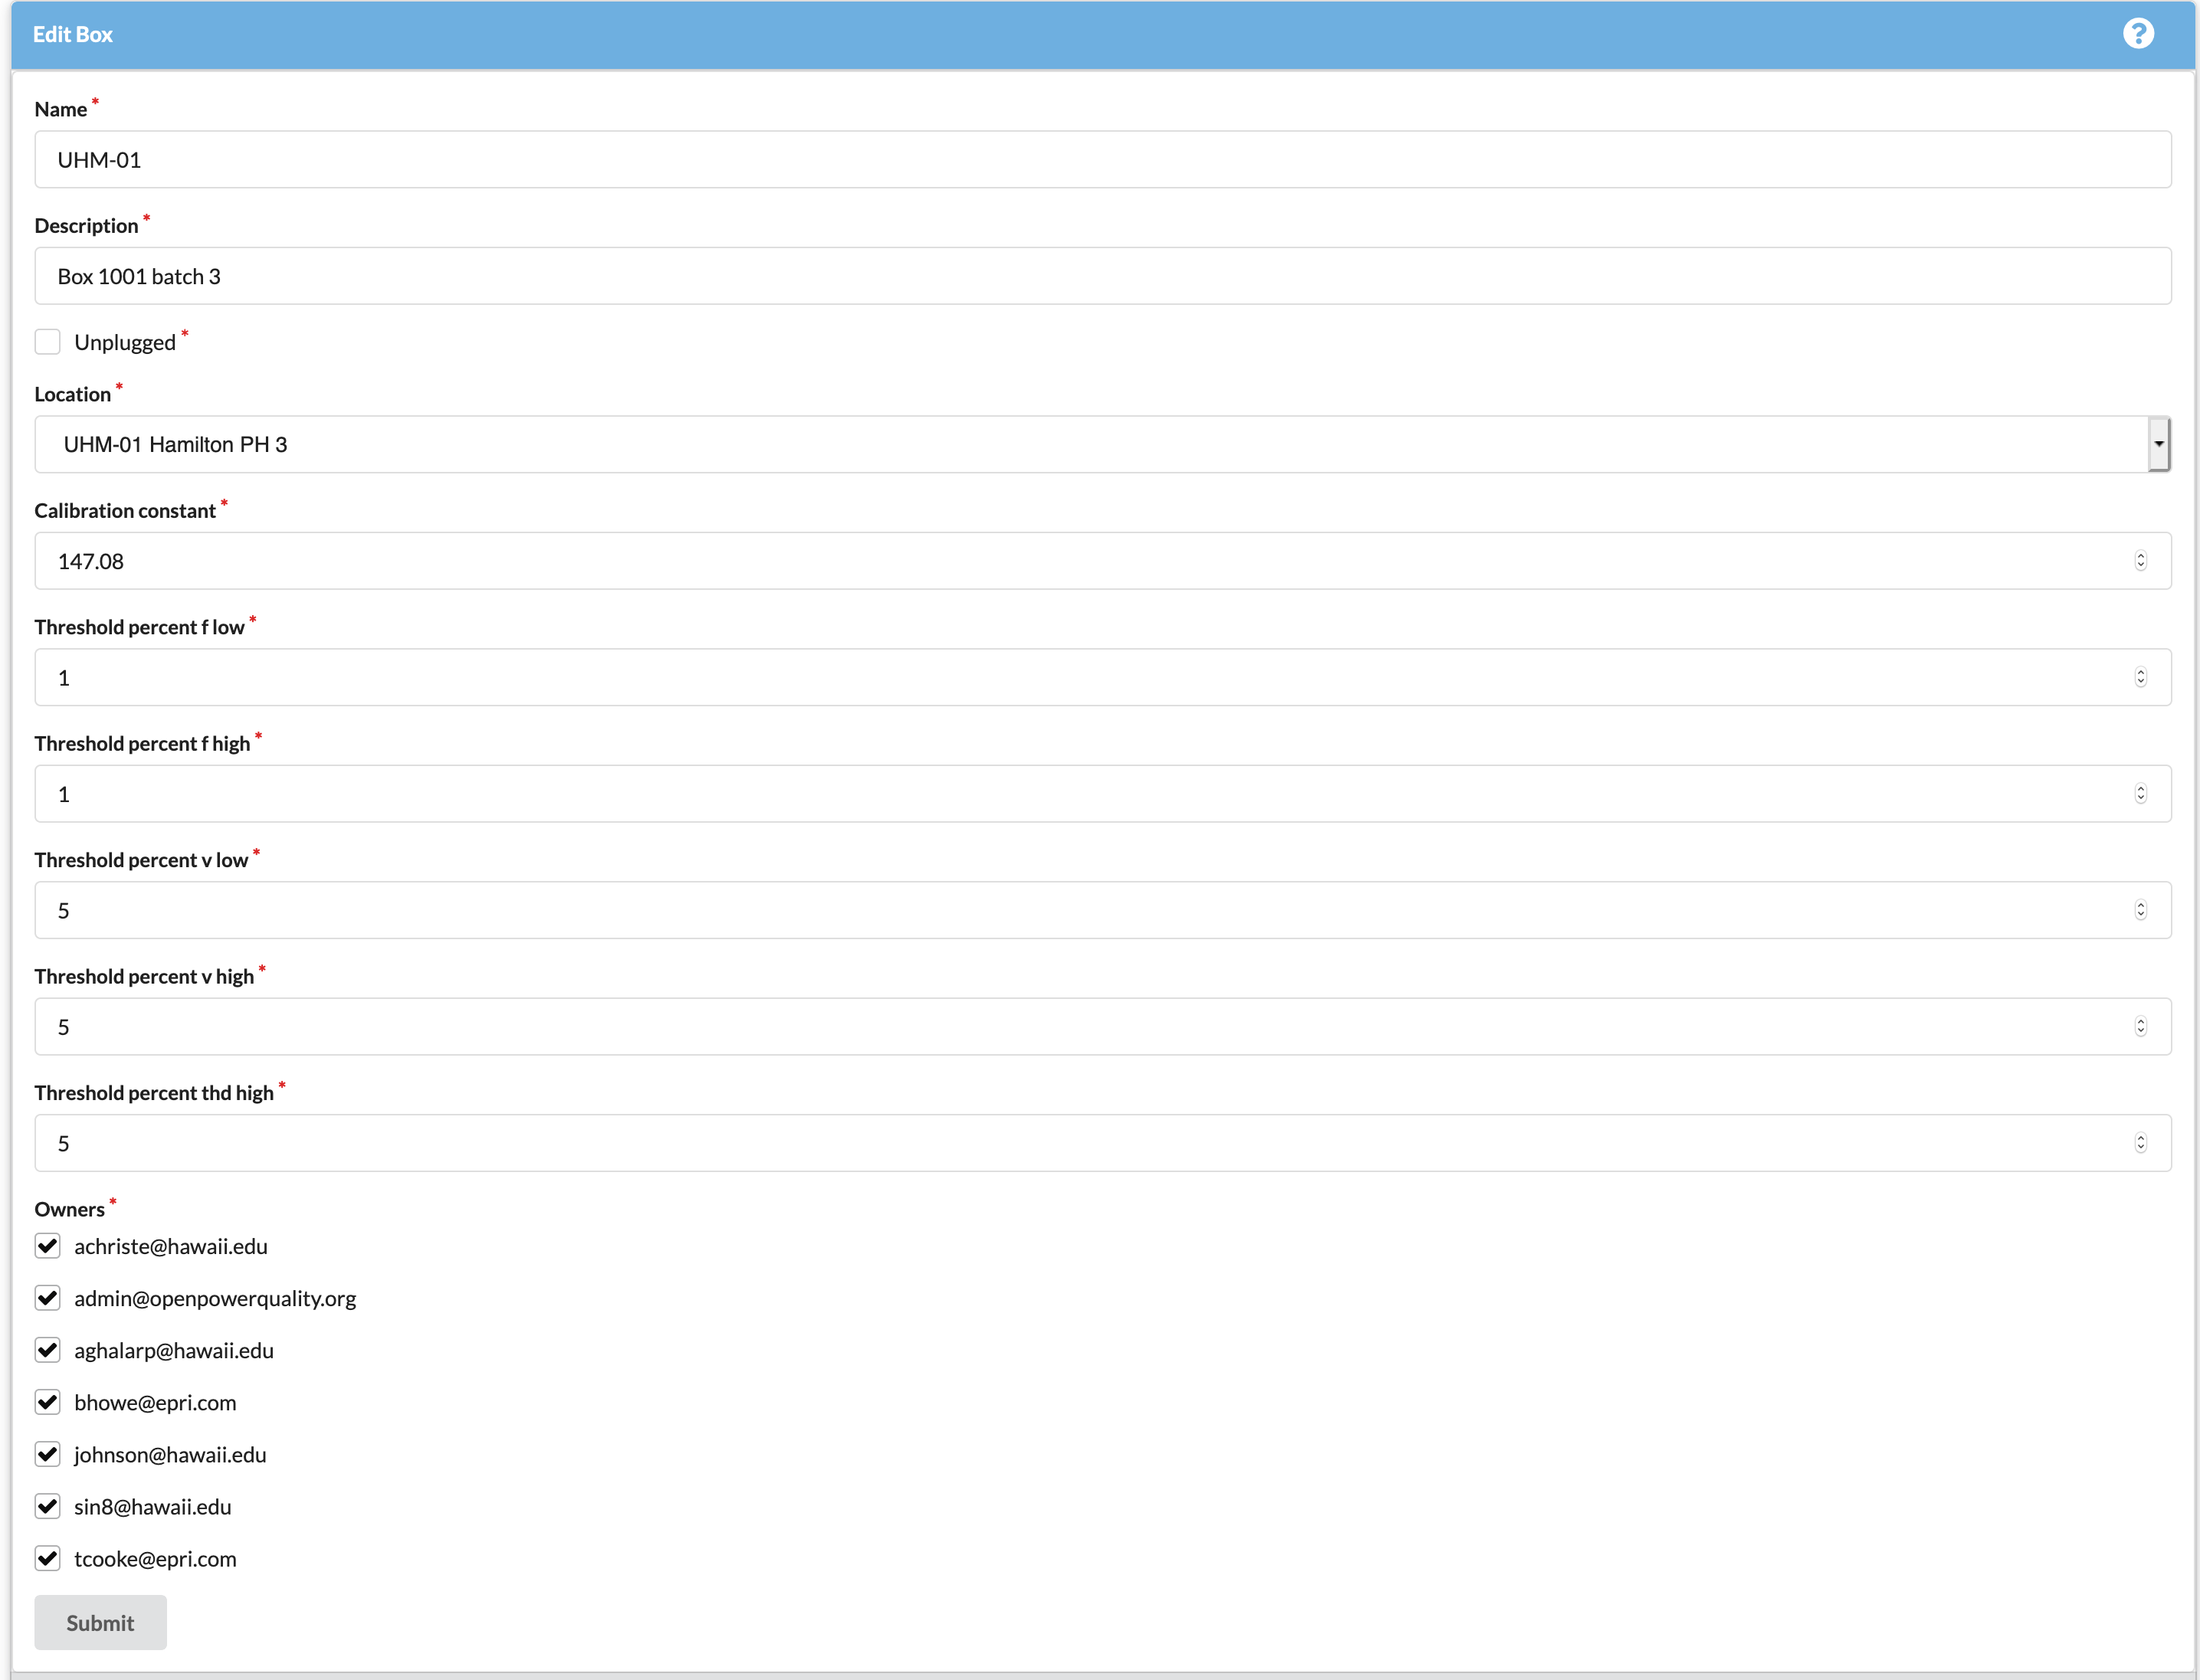
\includegraphics[width=1\linewidth]{figures/view_thresholds.png}
	\caption{OPQ View Threshold Configuration}\label{fig:view_thresholds}
\end{figure}

OPQ View also provides a display for Laha metrics that were collected by Mauka. This is described and shown in section~\ref{lbl:SystemStatsPlugin}.

\subsection{OPQ: Dockerfication}\label{subsec:opq:-dockerfication}
The OPQ system is made up of many separate services and technology stacks. Each service has its own build process and set of other services that it communicates with. In order to streamline the building and deployment of OPQ services, we implemented a containerized architecture user Docker and Docker Compose. This architecture allows us to track the version of each service and provide the OPQ Cloud system as a monolithic service managed by Docker. This greatly simplifies deployment of not just individual services, but deployment of the entire system as a whole.

Each OPQ service runs in its own Docker container. Each container is configured so that network access is restricted to only the other containers that it is allowed to communicate with. Docker also allows us to manage which ports are open to the outside world for any particular service.

Docker also restricts access to the filesystem. These features combined help to provide a secure environment for the execution of OPQ services.

The Docker architecture that OPQ uses is presented in Figure~\ref{fig:docker_deploy}.

\begin{figure}
	\centering
	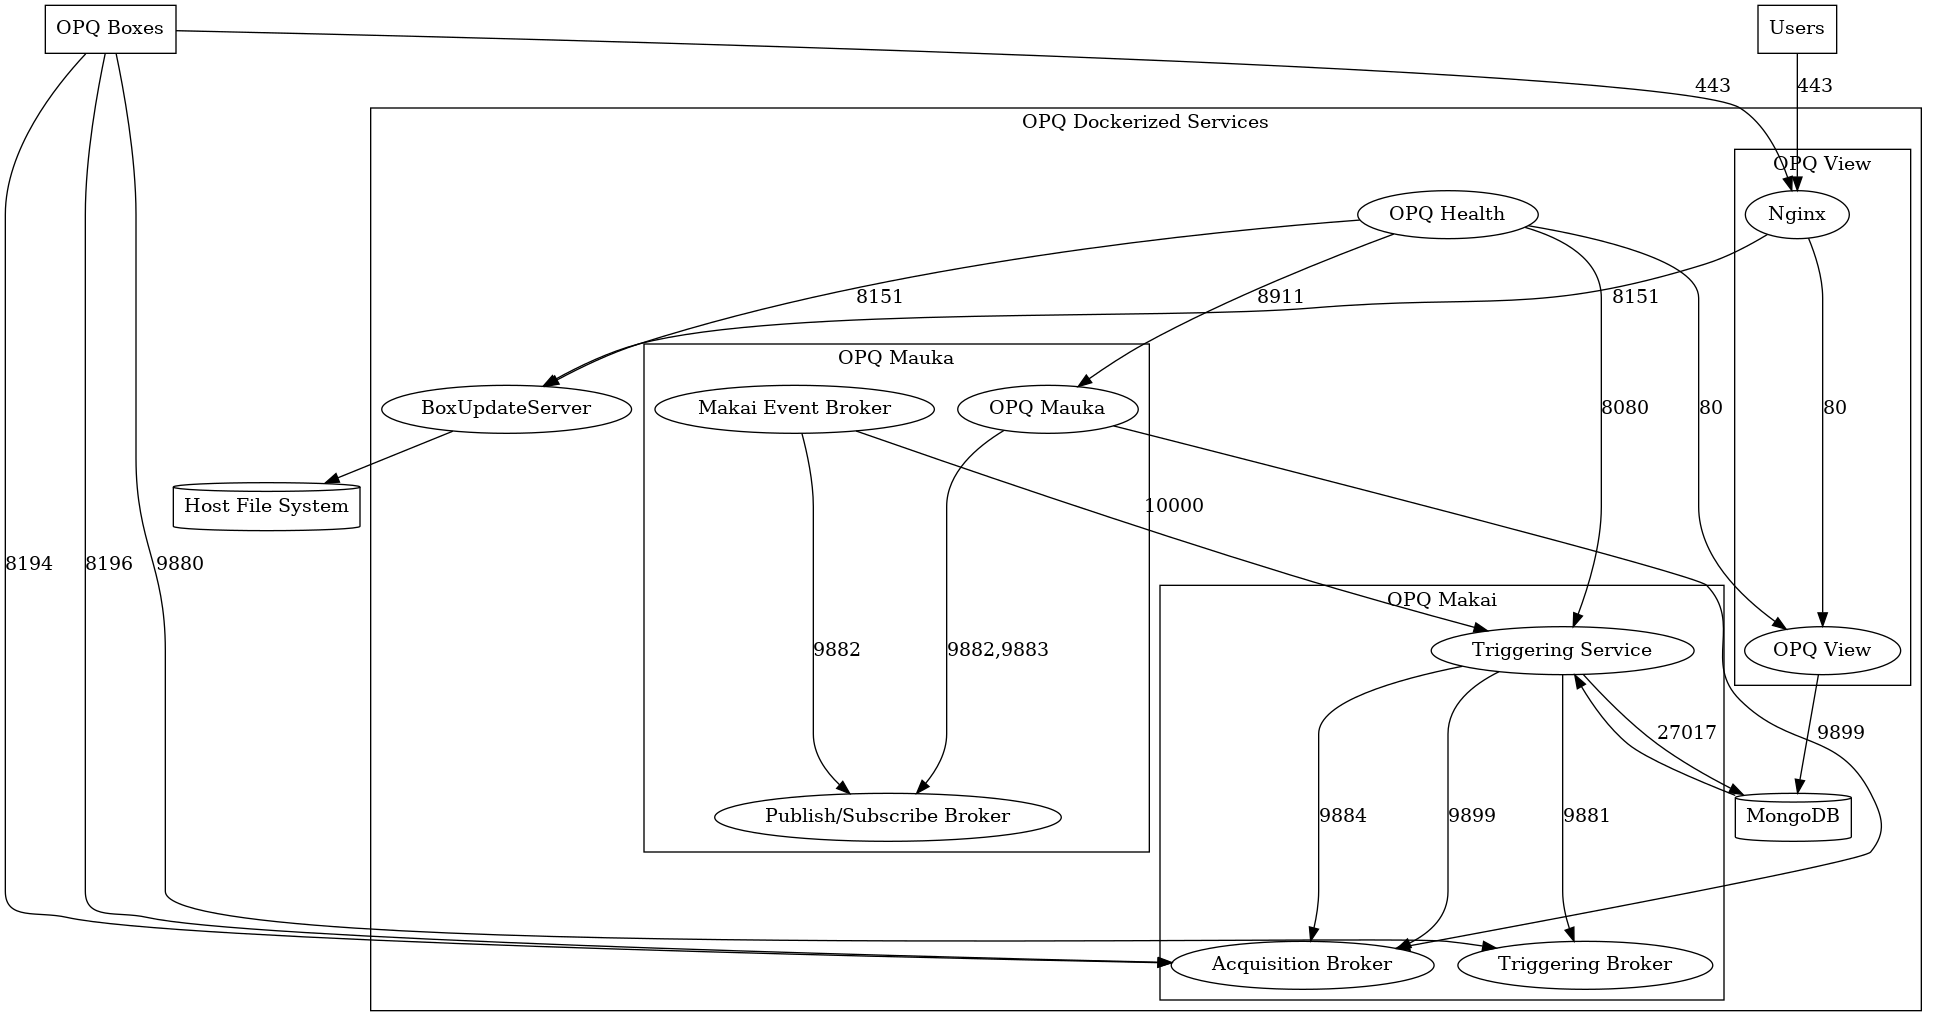
\includegraphics[width=1\linewidth]{figures/docker_deploy.png}
	\caption{OPQ Docker Architecture}\label{fig:docker_deploy}
\end{figure}

\section{Lokahi: A Laha-compliant Infrasound DSN}\label{sec:lokahi:-a-laha-compliant-infrasound-dsn}
Lokahi is a dynamic DSN that originally evolved as a distributed infrasound detection network. Infrasound is characterized as sound waves that are less than 20 Hz. Infrasound generally can not be deciphered by the human ear, but it can be detected using microphone and barometric pressure sensors. Any large movements of the atmosphere can produce infrasound. The Lokahi network was designed to supplement the International Monitoring System (IMS) for the capture  of undeclared and declared nuclear explosions. Lokahi has been successfully used to capture signals from volcanoes, hurricanes, aircraft, meteors, and other large atmospheric events.

Sensors in Lokahi are any mobile device that can run iOS or Android. We have sensors distributed world wide. The software stack for Lokahi consists of a distributed actor system for data acquisition, MongoDB for metadata persistence, Apache Kafka for data queues and interprocess communication, Python and related scientific libraries for analysis, and a distributed key-value store for long term storage or sensor data.

Recent development and improvements to the data API have allowed Lokahi to begin accepting data from any of the available onboard sensors on iOS and Android devices. Even though the main focus is still infrasound, having access to all of the available sensors provides the ability to sense other sensor fields and to perform interesting data fusion techniques.

A diagram of the Lokahi framework is provided in Figure~\ref{fig:lokahi}.


\begin{figure}
	\centering
	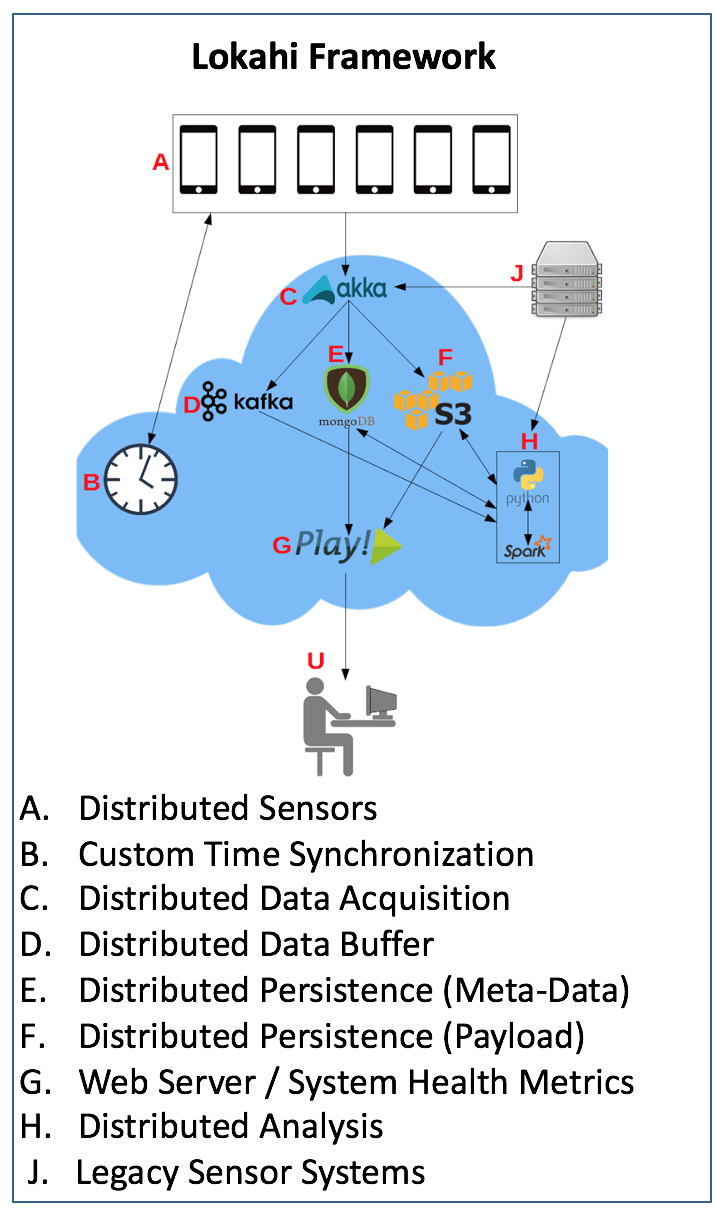
\includegraphics[]{figures/lokahi.png}
	\caption{Lokahi Design}\label{fig:lokahi}
\end{figure}

Lokahi is made up of several distributed services, each of which will be discussed in the following sections.

\subsection{Lokahi Data Acquisition Service}\label{subsec:lokahi-data-acquisition-service}
The data acquisition service is responsible for acquiring, authenticating, storing, and moving real-time sensor data from Lokahi sensors.

The data acquisition service is written in Rust and makes use of Actix Actors for scalability and distributed communication. Originally, the data acquisition server was written in Java using Akka Actors. I recently moved the acquisition server to Rust so that it can be ran on embedded hardware such as Raspberry Pis in resource restricted environments or on the edge of networks. Rust also provides performances improvements in terms of CPU utilization and memory utilization.

Type safe data is passed between actors where each actor fulfills a single purpose. When an actor successfully completes a unit of work, it responds with an empty success message to the calling actor. If an actor fails to complete a unit of work, it responds with a type safe error message to the calling actor. Errors messages are passed up the chain until they get to the original caller.

All actors in this service are optional and configurable. For instance, this service can be brought up with the sole purpose of writing the data to a file system and nothing else, or acting  solely as a data relay, or only storing data to AWS S3, or it can do it all.

Further, multiple Actors can be ran concurrently with different configurations. For instance, its possible to define multiple Kafka actors, each with their own encryption and endpoint configurations, or you could write data to multiple file systems by configuring multiple Fs Actors, etc.

It's also possible to configure each actor with whitelists and blacklists where items can be added by sensor id or sensor owner. In this way, the configuration for each actor can be fine tuned to only allow certain sensors or sets of sensors or disallow sets of sensors. This is utilized when we require that only a subset of data received be forwarded to a particular actor. For instance, when we share real time data with our collaborators, they are only interested in a certain subset of data that we are receiving. Therefore, we create a whilelist with their information so that they only receive the data they are interested in. On the other hand, that data may be sensitive, so we black list it on other actors so that data is not forwarded to those actors.

Finally, configuration of all actors is performed declaratively in a type safe configuration file.

Figure~\ref{fig:LokahiAcquisition} provides an overview of the workflow and communication between Actors with the acquisition service.

\begin{figure}
	\centering
	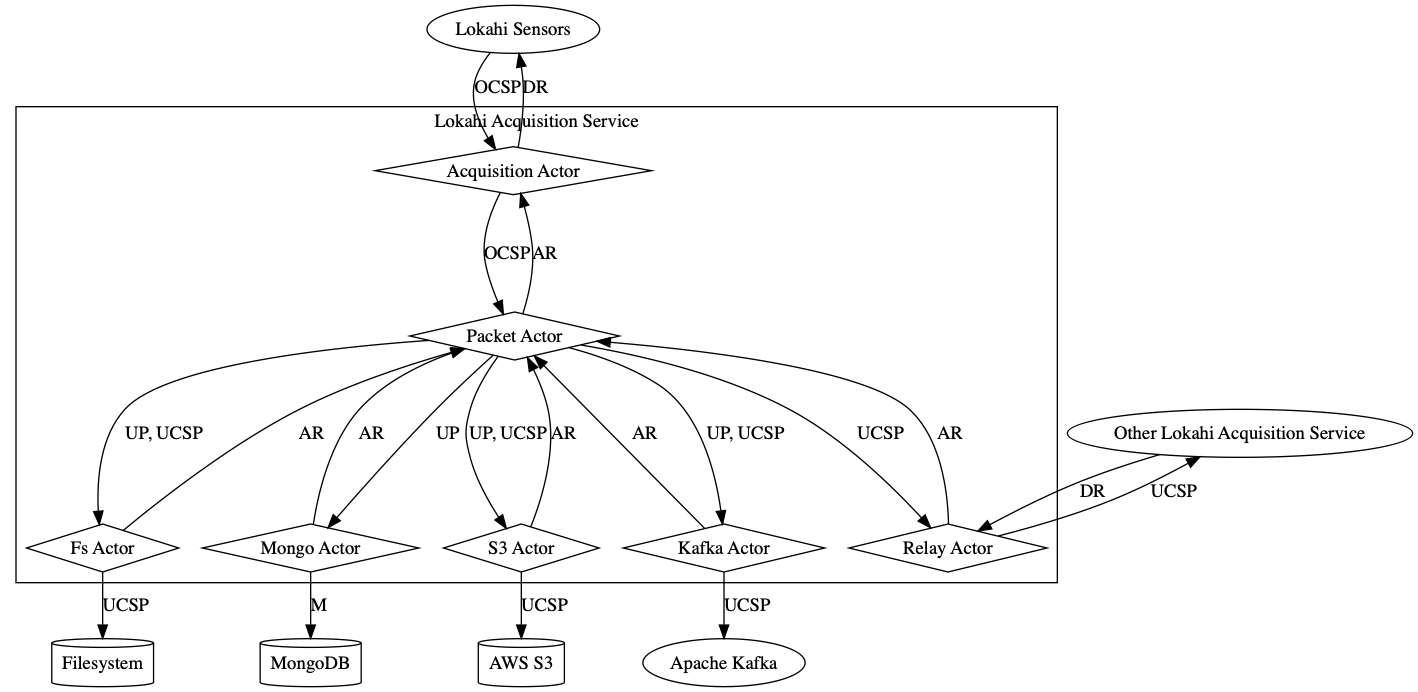
\includegraphics[width=\linewidth]{figures/lokahi_acquisition.png}
	\caption{Lokahi Acquisition Architecture where OCSP=``original compressed serialized packet", UP=``updated packet", UCSP=``updated compressed serialized packet", M=``metadata", AR=``actor response", DR=``device response".}
	\label{fig:LokahiAcquisition}
\end{figure}

\subsubsection{Acquisition Service Configuration}

Configuration for this service is stored in a .toml file. This file is parsed from the environment on service startup and deserialized into a typesafe Rust struct. The configuration is completely declarative and all actor configurations are optional. Also, it's possible to add new actors to this system by simply declaring a new actor in the configuration and restarting the service. This approach scales much more nicely than our previous approach which required editing the source code directly to modify or add actors.

An example configuration file with one of each actor type is provided in the appendix in section~\ref{lokahi_acquisition_config}.

\subsubsection{Acquisition Actor}
Lokahi sensors establish an encrypted WebSocket connection to the the acquisition server in which they send data over. Encryption is provided over standard HTTPS using Let's Encrypt as a certificate provider. Once the connection is established, the connection remains open for as long as the sensor is continuously sending data. Each connection causes the creation of a new Actix Actor within the acquisition service. Instead of creating a thread for each connection, actors share their resources over a configurable thread pool and lightweight green threads are used to provide concurrency. Since most of the work of the acquisition service is I/O bound, the use of green threads makes the most sense.

This actor is also responsible for checking the response messages from all actors in the acquisition pipeline. If all responses are ``Ok", then this actor responds to the sensor with a checksum and an ``Ok" response. If any of the actor responses are an error, then this actor responds to the sensor with an error message and the sensor will store the data onboard until it is able to send at a later time.

\subsubsection{Packet Actor}
The acquisition service ``Packet Actor" handles each packet from a sensor individually. When a packet arrives, the packet is first decompressed using a custom LZ4 compression protocol where the first four bytes of the compressed payload contain the size of the original uncompressed data.

Once the packet is decompressed, it is then deserialized using Protocol Buffers into a struct that Rust is able to work with. The data packet protocol is provided in full in the appendix in section~\ref{lokahi-data-packet-protocol}.

Each packet contains a Json Web Token (JWT) which is a cryptographically signed token generated by Lokahi Web. This token provides user authentication and authorization. The acquisition service extracts the token and either accepts or rejects the packet depending on if authentication is successful or not.

The acquisition service ``Packet Actor" performs several small updates to the packet when it arrives. First, it adds a server receive timestamp which marks the time that the packet was received at the server. This, along with the packet sensor time stamps allows us to keep a running record of latency values from sensors to acquisition service. Next, the authentication token and Firebase token are redacted since their values are only used within the acquisition service. This prevents others from accessing this data and masquerading as someone else. Finally, the packet is marked as either ``real-time" or ``backfilled" depending using a heuristic that compares the packet timestamps to the server timestamps. Real-time data is data that is recorded and immediately transferred over the network whereas backfilled data is recorded and sent over the network at a later time. Finally, the packet is updated with a data key which is the key that will eventually be used to store the data packet in AWS S3, a distributed key-value store.

\subsubsection{Mongo Actor}
Once the packet has been updated by the ``Packet Actor", all meta-data is extracted and stored in MongoDB by a ``Mongo Actor". Everything from the original packet is stored except for the data payloads themselves. However, the descriptive statistics of the payloads are stored so that the database contains some metadata about what the payload contains.

Multiple collections are updated by the Mongo Actor when a packet is received.

The ``RedvoxPacketApi900" collection stores metadata for all data packets received from sensors. The schema for this collection is described in Table~\ref{table:RedvoxPacketApi900}. This document also includes two embedded documents EvenlySampledChannel\ref{table:EvenlySampledChannel} and UnevenlySampledChannel\ref{table:UnevenlySampledChannel}. The EvenlySampledChannel document contains metadata for evenly sampled channels such as the microphone. The UnevenlySampledChannel document contains metadata for unevenly sampled channels such as barometer, location, gyroscope, accelerometer, etc.

\begin{table}[H]
	\centering
	\caption{RedvoxPacketApi900}
	\begin{tabular}{|c|c| p{7.5cm} |}
		\hline
		Field & Enum Value & Description  \\
		\hline
		\_id & bson.ObjectId & The object id associated with the document. \\
		\hline
		className & str & The class name used for Java serialization and deserialization. \\
		\hline
		api & int32 & The API version of this data (should be 900). \\
		\hline
		redvoxId & str & The id of the sensor. \\
		\hline
		redvoxUuid & str & The uuid of the sensor. \\
		\hline
		authenticatedEmail & str & The user account associated with this device. \\
		\hline
		authenticationToken & str & The JWT that was used for authenticating this packet. \\
		\hline
		firebaseToken & str & The firebase token associated with this device. \\
		\hline
		isBackfilled & bool & True if this packet was backfilled, False otherwise. \\
		\hline
		isPrivate & bool & True if this packet is marked as private, False otherwise. \\
		\hline
		isScrambled & bool & True if this packet has voice data scrambled, False otherwise. \\
		\hline
		deviceMake & str & The make of the sensor. \\
		\hline
		deviceModel & str & The model of the sensor. \\
		\hline
		deviceOs & str & The OS of the sensor (either iOS or Android). \\
		\hline
		deviceOsVersion & str & The OS version. \\
		\hline
		appVersion & str & The sensor app version. \\
		\hline
		batteryLevelPercent & f32 & The sensor's battery level. \\
		\hline
		deviceTemperatureC & f32 & The sensor's temperature in C. \\
		\hline
		acquisitionServer & str & The server that this data was sent to. \\
		\hline
		timeSynchronizationServer & str & The server this sensor used for synch. \\
		\hline
		authenticationServer & str & The server this sensor used to authenticated with. \\
		\hline
		appFileStartUsUtc & i64 & The timestamp of the start of this packet. \\
		\hline
		appFileStartMachine & i64 & The machine timestamp of the start of this packet. \\
		\hline
		serverTimestampUsUtc & i64 & The time that this packet was received at the server. \\
		\hline
		evenlySampledChannels & [EvenlySampledChannel] & Evenly sampled channels metadata. \\
		\hline
		unevenlySampledChannels& [UnevenlySampledChannel] & Unevenly sampled channels metadata. \\
		\hline
		metadata & [str] & A list of metadata added to this packet. \\
		\hline
		dataKey & str & The location of the original data file stored in AWS S3. \\
		\hline
	\end{tabular}
	\label{table:RedvoxPacketApi900}
\end{table}

\begin{table}[H]
	\centering
	\caption{RedvoxPacketApi900.EvenlySampledChannel}
	\begin{tabular}{|c|c| p{8cm} |}
		\hline
		Field & Enum Value & Description  \\
		\hline
		channelTypes & [str] & A list of sub-channels included in this channel. \\
		\hline
		sensorName & str & The name of sensor. \\
		\hline
		sampleRateHz & f64 & The sample rate of this sensor. \\
		\hline
		firstSampleTimestampUs & i64 & Timestamp of the first sample. \\
		\hline
		payloadCase & str & An enum string for the data type stored in the payload. \\
		\hline
		payloadCount & i32 & The number of items in the payload in the original data. \\
		\hline
		valueMeans & [f64] & List of mean values of the payload for each sub-channel. \\
		\hline
		valueStds & [f64] & List of the stddev of the values of the payload for each sub-channel. \\
		\hline
		valueMedians & [f64] & List of medians of the values of the payload for each sub-channel. \\
		\hline
		metadata & [str] & List of metadata added to this channel. \\
		\hline
	\end{tabular}
	\label{table:EvenlySampledChannel}
\end{table}

\begin{table}[H]
	\centering
	\caption{RedvoxPacketApi900.UnevenlySampledChannel}
	\begin{tabular}{|c|c| p{8cm} |}
		\hline
		Field & Enum Value & Description  \\
		\hline
		channelTypes & [str] & A list of sub-channels included in this channel. \\
		\hline
		sensorName & str & The name of sensor. \\
		\hline
		timestampsCount & i32 & The number of timestamps for this channel in the original data. \\
		\hline
		payloadCase & str & An enum string for the data type stored in the payload. \\
		\hline
		payloadCount & i32 & The number of items in the payload in the original data. \\
		\hline
		valueMeans & [f64] & List of mean values of the payload for each sub-channel. \\
		\hline
		valueStds & [f64] & List of the stddev of the values of the payload for each sub-channel. \\
		\hline
		valueMedians & [f64] & List of medians of the values of the payload for each sub-channel. \\
		\hline
		sampleIntervalMean & f64 & The mean sample interval of each sample. \\
		\hline
		sampleIntervalStd & f64 & The mean sample stddev of each sample. \\
		\hline
		sampleIntervalMedian & f64 & The median sample interval of each sample. \\
		\hline
		metadata & [str] & List of metadata added to this channel. \\
		\hline
	\end{tabular}
	\label{table:UnevenlySampledChannel}
\end{table}

The Mongo Actor also updates other documents which are used by Lokahi View for display, device, and user management. The schemas for these collections are described next.

The ``RedvoxDeviceApi900" collection contains metadata relating to each sensor that Lokahi receives from. This collection is described in Table~\ref{table:RedvoxDeviceApi900}. This collection also contains two embedded documents ``PrivacyPolicy"\ref{table:PrivacyPolicy} and ``AuthenticatedEmailEntry"\ref{table:AuthenticatedEmailEntry}.

\begin{table}[H]
	\centering
	\caption{RedvoxDeviceApi900}
	\begin{tabular}{|c|c| p{8cm} |}
		\hline
		Field & Enum Value & Description  \\
		\hline
		\_id & bson.ObjectId & The object id of this document. \\
		\hline
		className & str & Used for Java ORM interop. \\
		\hline
		redvoxId & str & The id associated with this device. \\
		\hline
		uuid & str & The uuid associated with this device. \\
		\hline
		lastUpdatedTimestamp & i64 & The timestamp of the last time this device received data. \\
		\hline
		lastPacket & DBRef & A reference to the last received packet. \\
		\hline
		lastLocationPoint & mongo.Point & The last location this device was received from. \\
		\hline
		currentPolicyType & str & The devices policy type (public/private). \\
		\hline
		privacyPolicies & [PrivacyPolicy] & A list of privacy policies this device has used. \\
		\hline
		currentAuthenticatedEmail & str & This devices current user. \\
		\hline
		authenticatedEmailEntries & [AuthenticatedEmailEntry] & A list of all users who have used this device. \\
		\hline
		valid & bool & A field that marks this device as valid or invalid. \\
		\hline
		receivers & [str] & A list of users who can access data from this device. \\
		\hline
	\end{tabular}
	\label{table:RedvoxDeviceApi900}
\end{table}

\begin{table}[H]
	\centering
	\caption{PrivacyPolicy}
	\begin{tabular}{|c|c| p{8cm} |}
		\hline
		Field & Enum Value & Description  \\
		\hline
		policyType & str & A string representing the policy type (public/private). \\
		\hline
		startTimestampMillisecondsSinceEpochUtc & i64 & Start time of this policy. \\
		\hline
	\end{tabular}
	\label{table:PrivacyPolicy}
\end{table}

\begin{table}[H]
	\centering
	\caption{AuthenticatedEmailEntry}
	\begin{tabular}{|c|c| p{8cm} |}
		\hline
		Field & Enum Value & Description  \\
		\hline
		authenticatedEmail & str & The email associated with this account at this time. \\
		\hline
		startTimestampMillisecondsSinceEpochUtc & i64 & Start time of this email entry. \\
		\hline
	\end{tabular}
	\label{table:AuthenticatedEmailEntry}
\end{table}

The ``HistoricalDevice" collection is used to store metadata about the last data that was received for each sensor. This is used in Lokahi View for displaying the location of every sensor ever received. The HistoricalDevice collection is described in Table~\ref{table:HistoricalDevice}.

\begin{table}[H]
	\centering
	\caption{HistoricalDevice}
	\begin{tabular}{|c|c| p{8cm} |}
		\hline
		Field & Enum Value & Description  \\
		\hline
		deviceId & i64 & The sensor id. \\
		\hline
		uuid & i64 & The sensor uuid. \\
		\hline
		lastActive & Date & The last time this device was active. \\
		\hline
		lastLocation & mongodb.Point & The last location this device was received from. \\
		\hline
		os & str & The OS of this device as of its last sent packet. \\
		\hline
	\end{tabular}
	\label{table:HistoricalDevice}
\end{table}

The ``DailyDataUsage" collection is a collection that stores metadata relating to how much data is used daily per user of the Lokahi service. The ``DailyDataUsage" document schema is provided in Table~\ref{table:DailyDataUsage}.

\begin{table}[H]
	\centering
	\caption{DailyDataUsage}
	\begin{tabular}{|c|c| p{8cm} |}
		\hline
		Field & Enum Value & Description  \\
		\hline
		\_id & bson.ObjectId & The object id of this document. \\
		\hline
		user & str & The user account associated with this document. \\
		\hline
		year & int32 & The year of this document. \\
		\hline
		month & int32 & The month of this document. \\
		\hline
		day & int32 & The day of this document. \\
		\hline
		bytesContributed & int64 & The number of bytes contributed by this user. \\
		\hline
		bytesConsumed & int64 & The number of bytes consumed by this user. \\
		\hline
	\end{tabular}
	\label{table:DailyDataUsage}
\end{table}

\subsubsection{S3 Actor}
After the metadata has been stored, the updated packet is serialized back into bytes and then compressed using the same custom LZ4  compression protocol. This data is then sent to AWS S3 by the ``S3 Actor" for permanent storage for later data retrieval. S3 is a cloud service offered by Amazon which acts as a distributed key-value store with essentially unlimited space.

%Data is stored to S3 using using the following directory layout: api900/[YYYY]/[MM]/[DD]/[sensor\_id]_[packet\_timestamp\_ms].rdvxz.

\subsubsection{Fs Actor}
The data can optionally be stored to any accessible file system using the ``Fs Actor". This is useful in cases when your acquisition server may only have local network access, such as restricted sites with an acquisition server running on a Raspberry Pi on a LAN\@.

\subsubsection{Kafka Actor}
The compressed data is next produced to several Apache Kafka endpoints using the ``Kafka Actor".

Apache Kafka provides a distributed messaging queue that can use publish/subscribe semantics. Lokahi uses Kafka for inter-process distributed communication and for providing a real-time data endpoint for our collaborators. Lokahi manages an internal Kafka queue that acts as a ring buffer for storing an hours worth of real-time data for each device. This real-time ring buffer is used for generating real time plots of data without needing to access the database or pull the data from AWS S3.

Lokahi also provides secure real-time Kafka endpoints to our collaborators which include national labs, defense contractors, and private contracts. The acquisition service filters collaborator packets based off of the JWT and encrypts the compressed serialized packet with the collaborator's GPG public key. Our collaborators then use an Apache NiFi service for collecting and decrypting the data from the Kafka endpoint for their own internal use.

Each device is provided its own partition within Kafka to publish data to. Since each Kafka partition creates a file on the file system, the number of Kafka partitions and the partitions themselves must be managed intelligently. Partitions are assigned by the acquisition service. The acquisition service looks up the next available partition in the database. Partitions become available if a sensor stops using a partition for longer than an hour. Our current design provides up to 500 concurrent partitions at once.

\subsubsection{Relay Actor}
The acquisition service can act as a relay to other acquisition services that speak the same protocol. If this actor is enabled, any packets it receives are relayed to the configured acquisition server. This is useful for load balancing and for timing accuracy. In load balancing, this server can be configured to filter subsets of devices to other acquisition servers by configuring a relay actor for each server that data is being forwarded to. For timing accuracy, this service can be deployed on a Raspberry Pi at the edge of a network near the sensors, reducing the latency between sensor and server. Then, when a packet arrives at the server, it is updated with a low latency server timestamp which improves timing accuracy. The low powered Raspberry Pi can then relay the packet to the cloud where it will be handled, but already have the improved timing accuracy built into the packet.

\subsection{Lokahi Time Synchronization}\label{subsec:lokahi-time-synchronization}
Much of Lokahi's sensor analysis requires that sensors be synchronized in time. In order to calculate direction and distance to a signal source, sensors should have clocks that are synchronized within milliseconds of each other. We initially tried to use NTP, but it did not provide the timing accuracy we desired, and thus, implemented a custom time synchronization protocol.

The protocol used in Lokahi is an implementation described by Tian et al in their Tri-Message Exchange paper\cite{tian2009tri}. This algorithm was developed specifically for providing accurate time synchronization in high latency networks.

This service is written in Rust and utilizes encrypted x for communication with sensors. While a sensor is recording data, a separate thread on that sensor continuously performs message exchanges with this service. The best exchange out of a group of exchanges (the one with the lowest latency) is then used to correct timing for packets.

A description of the algorithm is provided below. This algorithm expects that the client will build up a successive message exchange consisting of the elements B0, B1, B2, B3, A1, A2, A3, but only up two a maximum of two timestamps are ever exchanged at one time. These coefficients are then stored in each data packet so that the server can use them to correct for timing.

\begin{enumerate}
	\item Client connects to redvox-synch-server over WebSocket connection
	\item Client records and stores B0 immediately before sending message
	\item Client sends binary message to server where the payload is a single byte 0x00
	\item Server responds asynchronously, goto 5
	\item onMessage fires for client
	\begin{enumerate}
		\item Client records Btmp
		\item Client decodes payload (see protocol below)
		\item If sequence number is 0, then
		\begin{enumerate}
			\item Client extracts and stores A1 from server receive timestamp
			\item Client stores B1 = Btmp
			\item Client records and stores B2 immediately before sending message
			\item Client sends binary message to server where payload is a single byte 0x01
			\item Server responds asynchronously, goto 5
		\end{enumerate}
		\item If sequence number is 1, then
		\begin{enumerate}
			\item Client extracts and stores A2 from server receive timestamp
			\item Client extracts and stores A3 from server send timestamp
			\item Client stores B3 = Btmp
			\item Client can close the connection or reuse the same connection to perform another message exchange starting from 2
		\end{enumerate}
	\end{enumerate}
\end{enumerate}

The protocol used for communicating message exchanges is a simple binary protocol designed to reduce bandwidth. The protocol is described in detail in Table~\ref{table:syncproto}.

\begin{table}[H]
	\centering
	\caption{Time Synchronization Binary Protocol}
	\begin{tabular}{|c|c|c|}
		\hline
		Byte Offset & Size & Description \\
		\hline
		0 & 1 & Sequence Number (0 or 1) \\
		\hline
		1 &  8 & Int timestamp A $\mu\sec$  \\
		\hline
		9 & 8 & Int timestamp B $\mu\sec$ \\
		\hline
	\end{tabular}
	\label{table:syncproto}
\end{table}

\subsection{Lokahi Health}\label{subsec:lokahi-health}
System health is provided by three open source components Prometheus, Grafana, and node\_exporter. Prometheus is a time series database for metric collection and Grafana is a visualization solution for time series databases. ``node\_exporter" is installed on each system for collecting system statistics and sending them to a Prometheus endpoint. With these three systems, we are able to provide coverage for all performance metrics required by Lokahi.

\subsubsection{Up/Down Metrics}
node\_exporter, other than collecting system statistics, provides a simple metric for whether or not a system or service is up or down. This provides a base line of performance metrics. When a system goes down, an e-mail alert is sent to all interested parties. An example of our Up/Down interface is provided in Figure~\ref{fig:updown}.

\begin{figure}
	\centering
	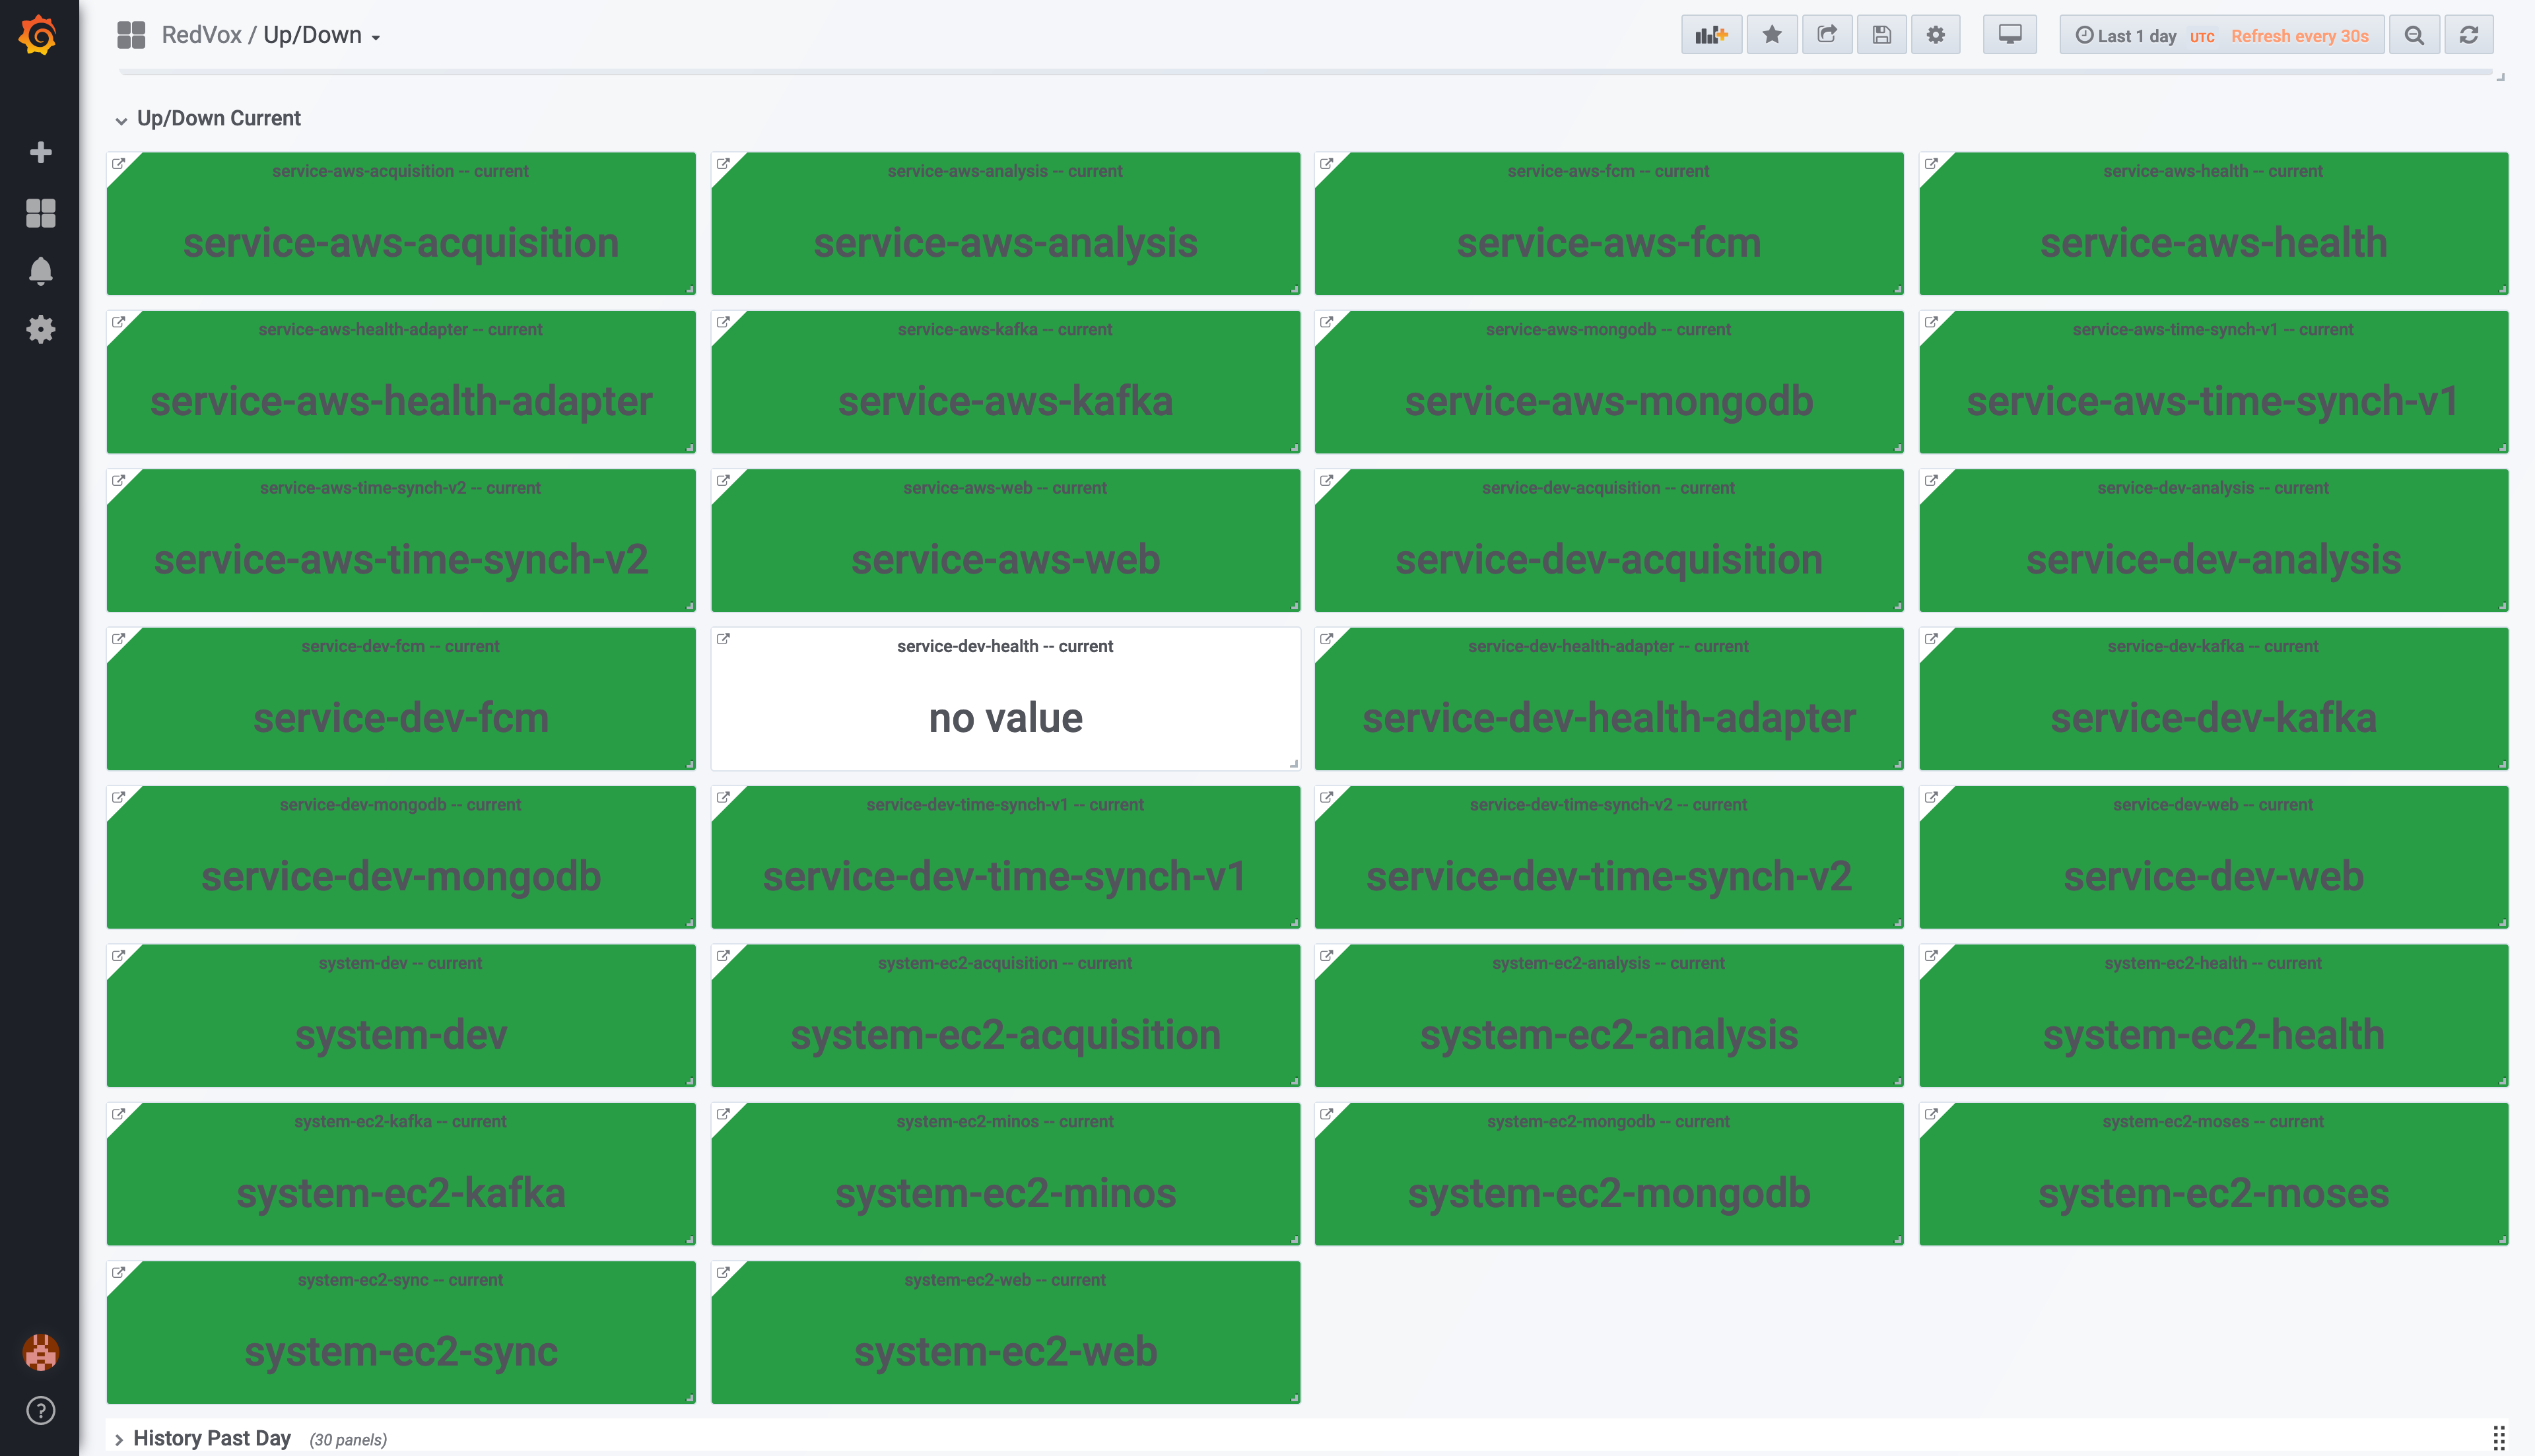
\includegraphics[width=\linewidth]{figures/updown.png}
	\caption{System and Service Status}
	\label{fig:updown}
\end{figure}

It's also possible to display a historic view up Up/Down metrics as shown in Figure~\ref{fig:updownhist}.

\begin{figure}
	\centering
	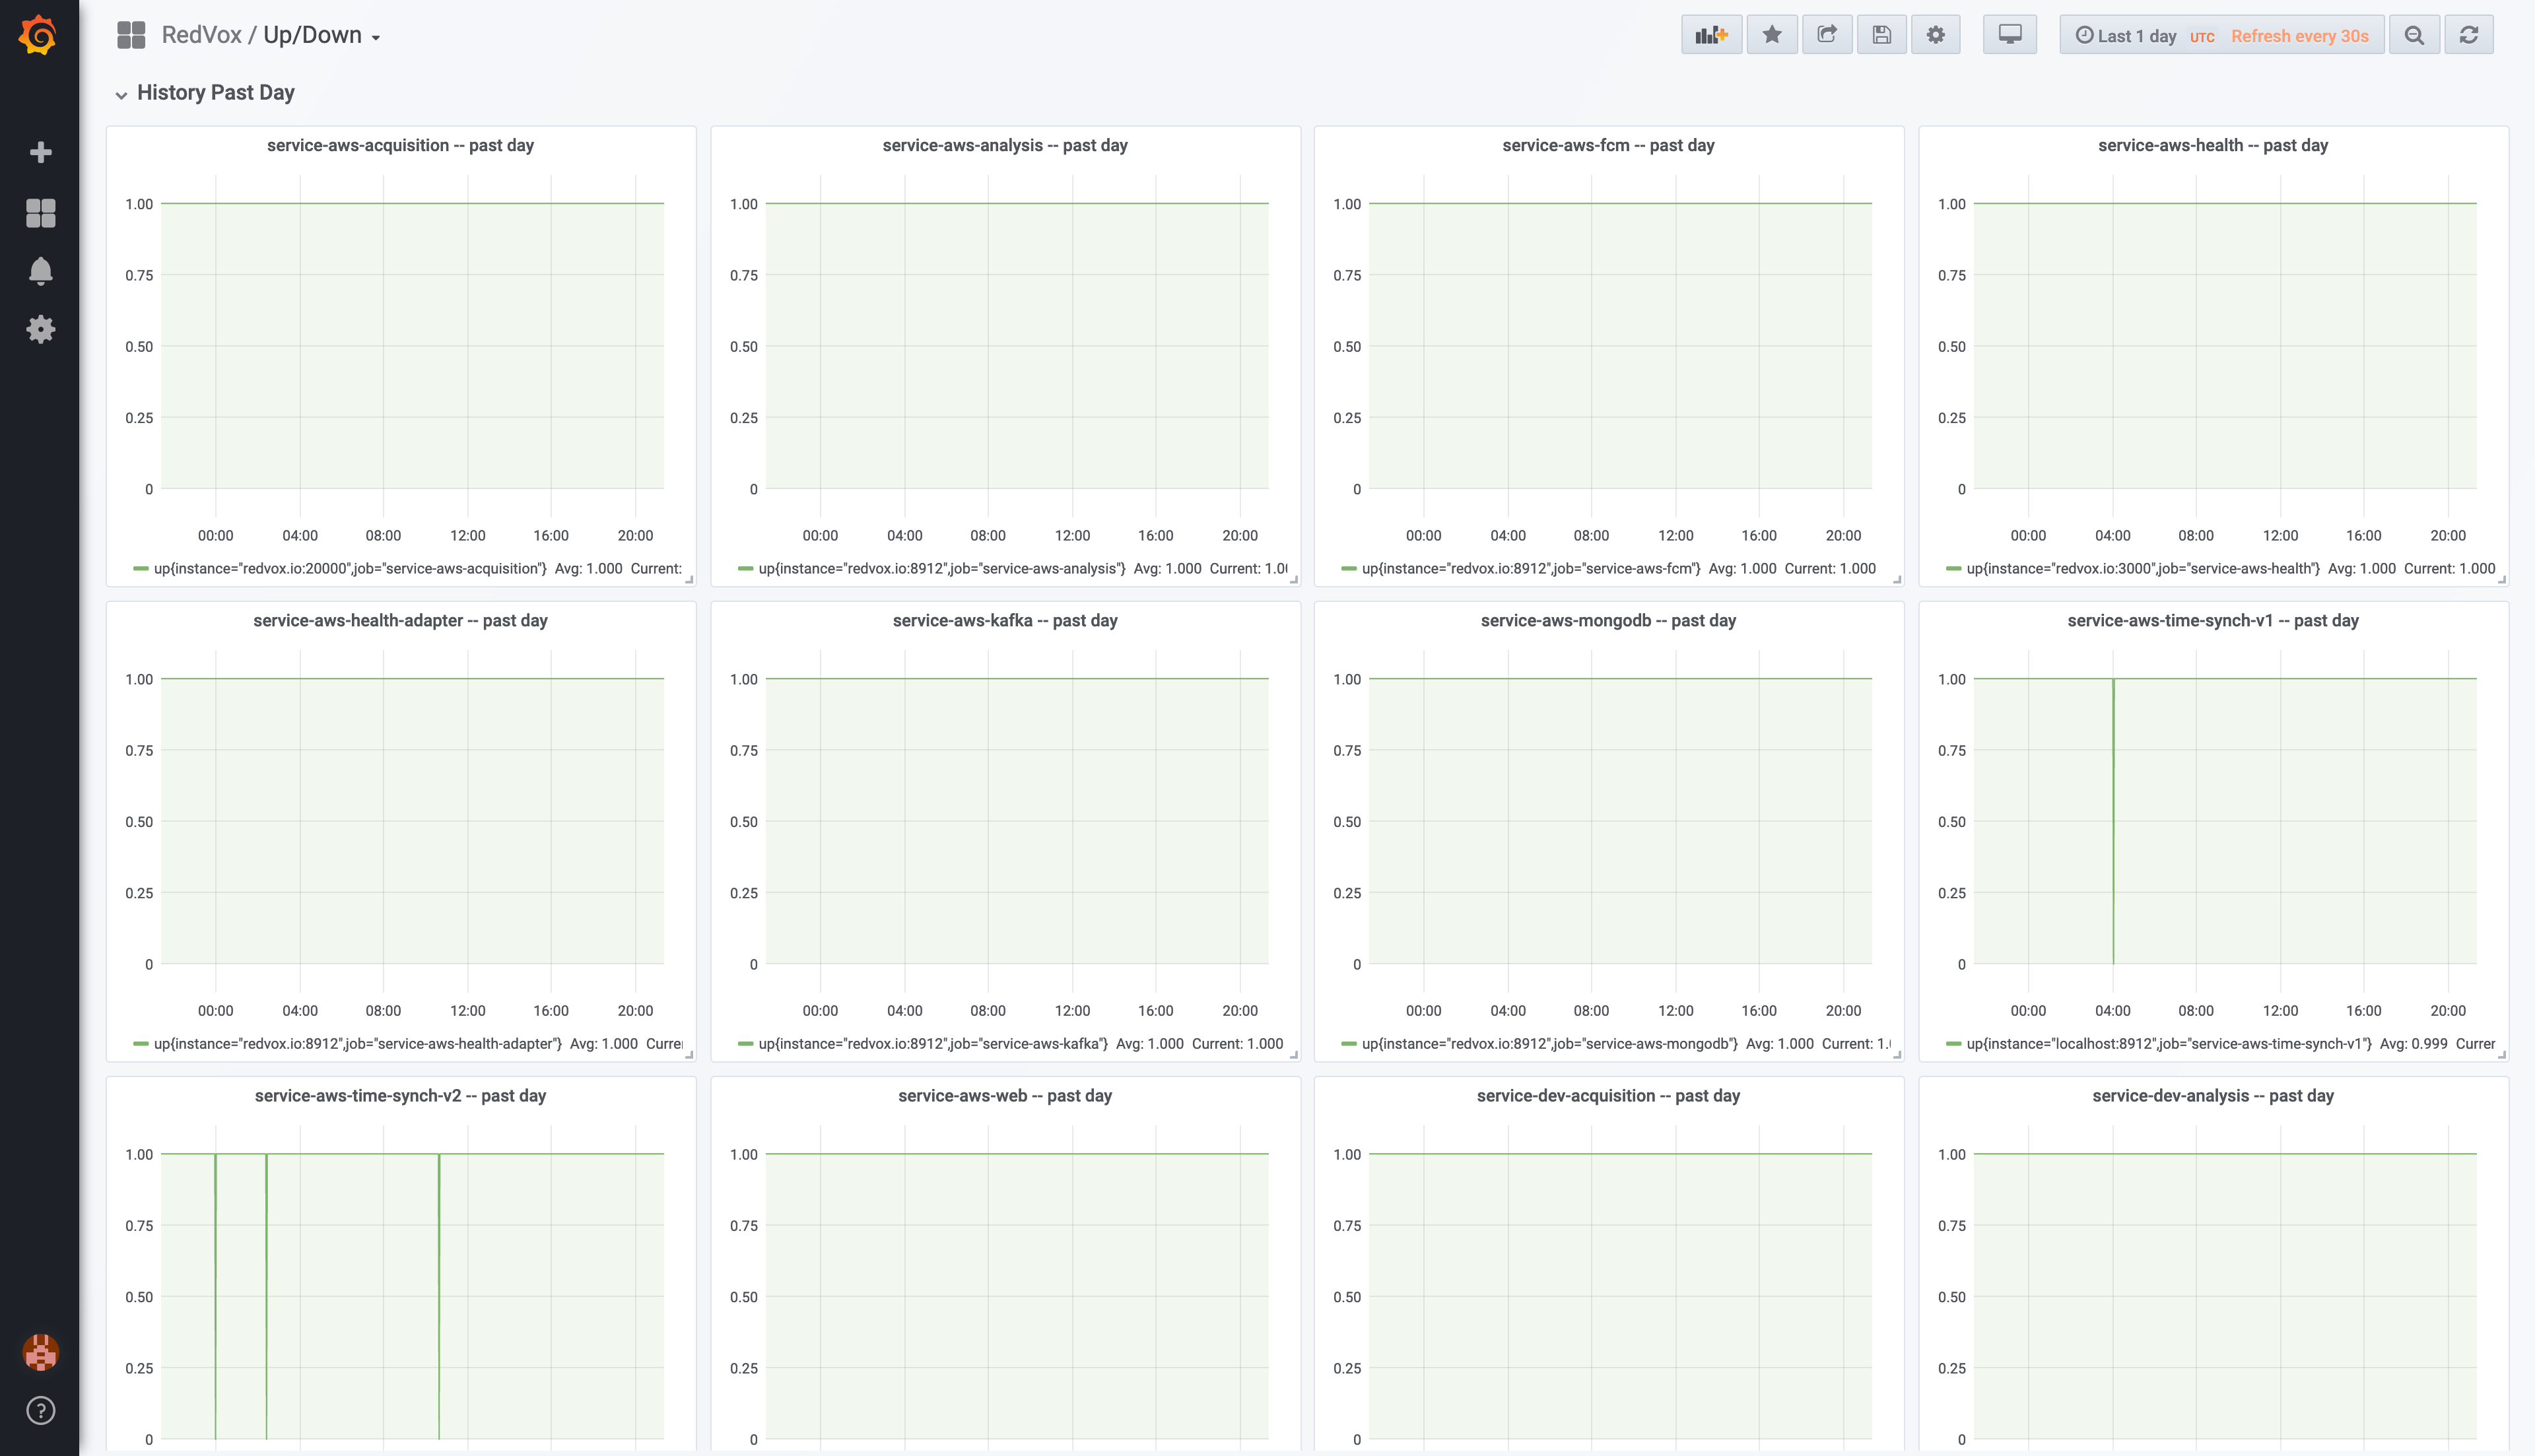
\includegraphics[width=\linewidth]{figures/updownhist.png}
	\caption{System and Service Status History Past Day}
	\label{fig:updownhist}
\end{figure}

\subsubsection{System Metrics}

``node\_exporter" provides Prometheus with a large selection of system metrics. We collect these metrics for each virtual server that we are running. We collect metrics on file system usage, memory usage, CPU usage, and network usage. An example of this from one of our services is displayed in Figure~\ref{fig:systemstats}.

\begin{figure}
	\centering
	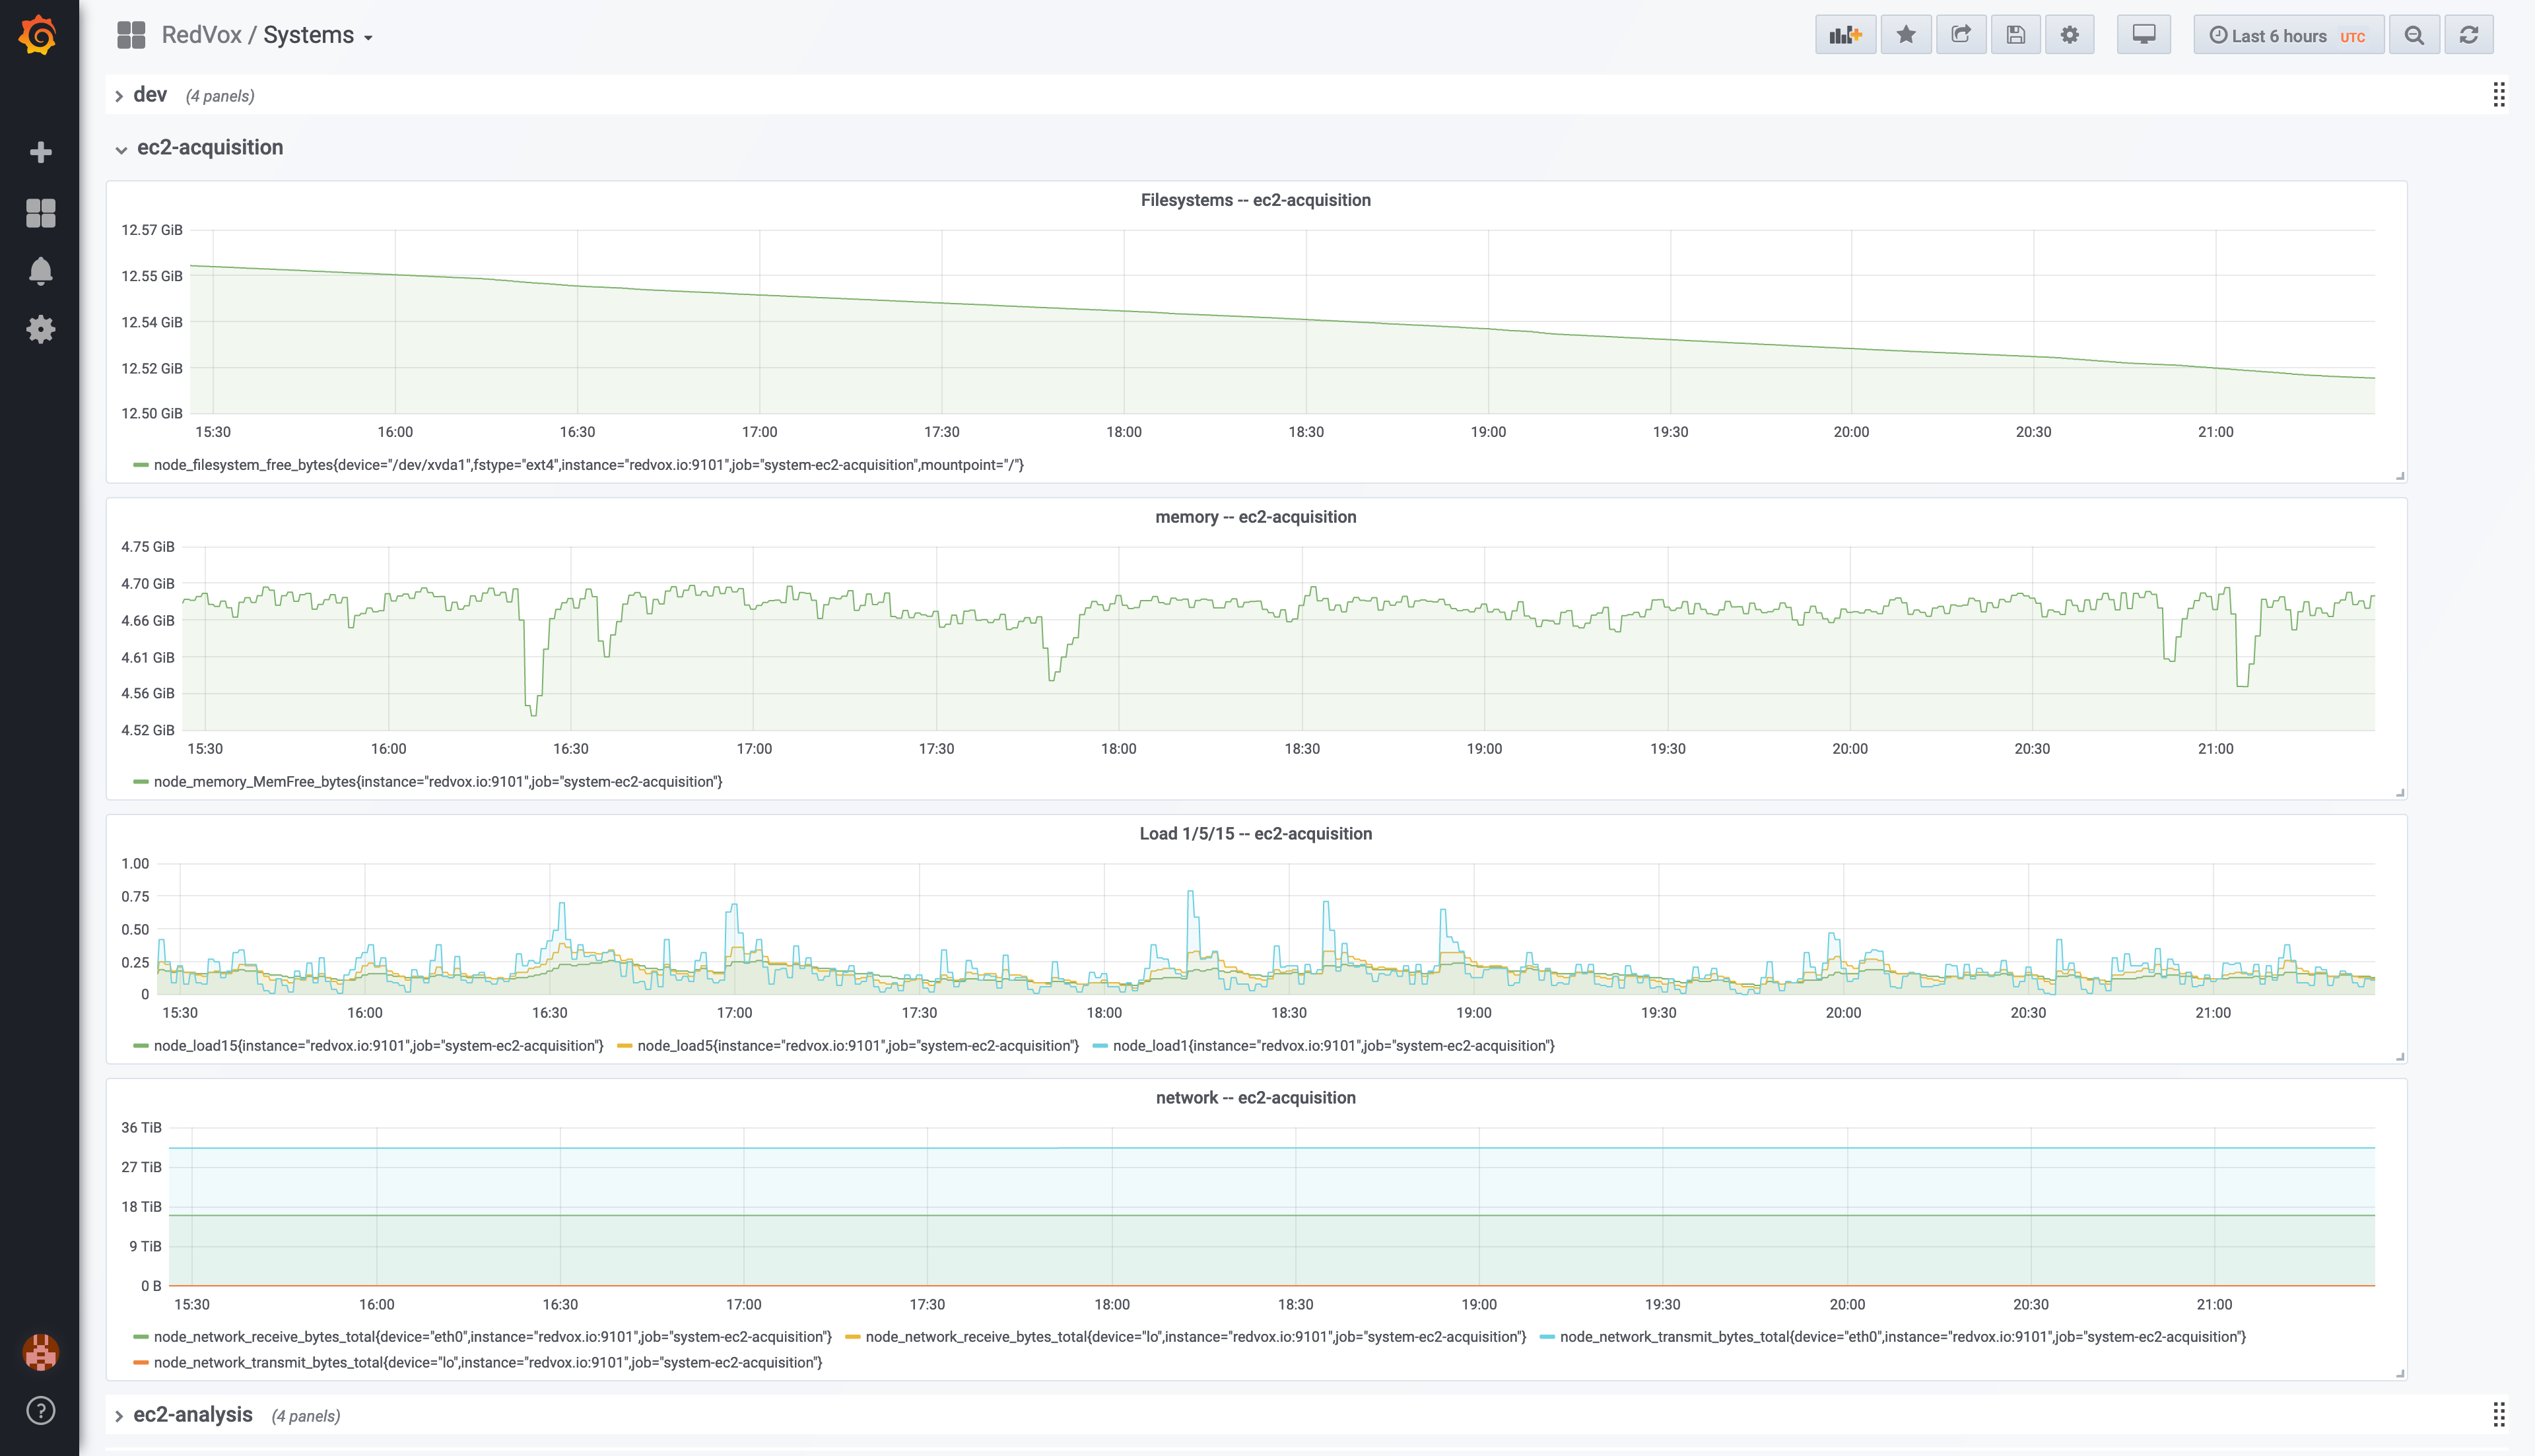
\includegraphics[width=\linewidth]{figures/systemstats.png}
	\caption{System Metrics}
	\label{fig:systemstats}
\end{figure}

\subsubsection{Sensor Metrics}

Lokahi also collects metrics from devices grouped by device and also grouped by device owner. We collect metrics on number of packets received and number of bytes received. We also collection metrics on sensor metadata such as device make/model, operating system, and app version. Due to the sensitive nature of this data, I will not provide a screenshot of these metrics. However, they are line graphs similar the system metrics.

\subsection{Lokahi Analysis}\label{subsec:lokahi-analysis}
Analysis of sensor data is provided by a custom Python framework. This framework utilizes an Apache Kafka client to subscribe to data request topics and real-time data topics.

When a request for analysis is received, the analysis framework will create a new process pool to run all of the analysis. Once the analysis is completed, the process pool is destroyed freeing up memory leaks caused by matplotlib. Requests for analysis include a time window, the devices that should be included for analysis, and the types of analysis that should be performed for those devices.

If the request is for real-time data, then the process will acquire the data from the Kafka real-time ring buffer data queue. If the request is for historic data, then the associated data will be looked up in the MongoDB database, and then the data payloads will be retrieved from AWS S3.

When the analysis is completed, metadata data about the analysis is stored to MongoDB, any figures generated by analysis are stored to AWS S3, and a response is sent back to Lokahi Web with the results of the analysis.

Lokahi Analysis is capable of creating the following products from sensor data:

\begin{itemize}
	\item Linear Microphone Waveform and FFT
	\item Log Microphone Waveform and FFT
	\item Multiresolution Microphone
	\item Barometer FFT
	\item Multiresolution Barometer
	\item Latency statistical line plot
	\item Location (latitude, longitude, altitude, speed) statistical line plot
	\item Magnetometer Waveform and FFT
	\item Gyroscope Waveform and FFT
	\item Accelerometer Waveform and FFT
	\item Light Waveform and FFT
\end{itemize}

Figures are generating using Python's matplotlib library. Most of the sensor analysis was implemented by colleagues at the Infrasound Laboratory in Kailua-Kona. I merely provided the infrastructure that allows them to run their geophysical analysis.

The analysis framework is not only capable of producing new reports and products, but can also be used to update existing reports and products.

An overview of the analysis architecture is provided in Figure~\ref{fig:analysis_architecture}.

\begin{figure}
	\centering
	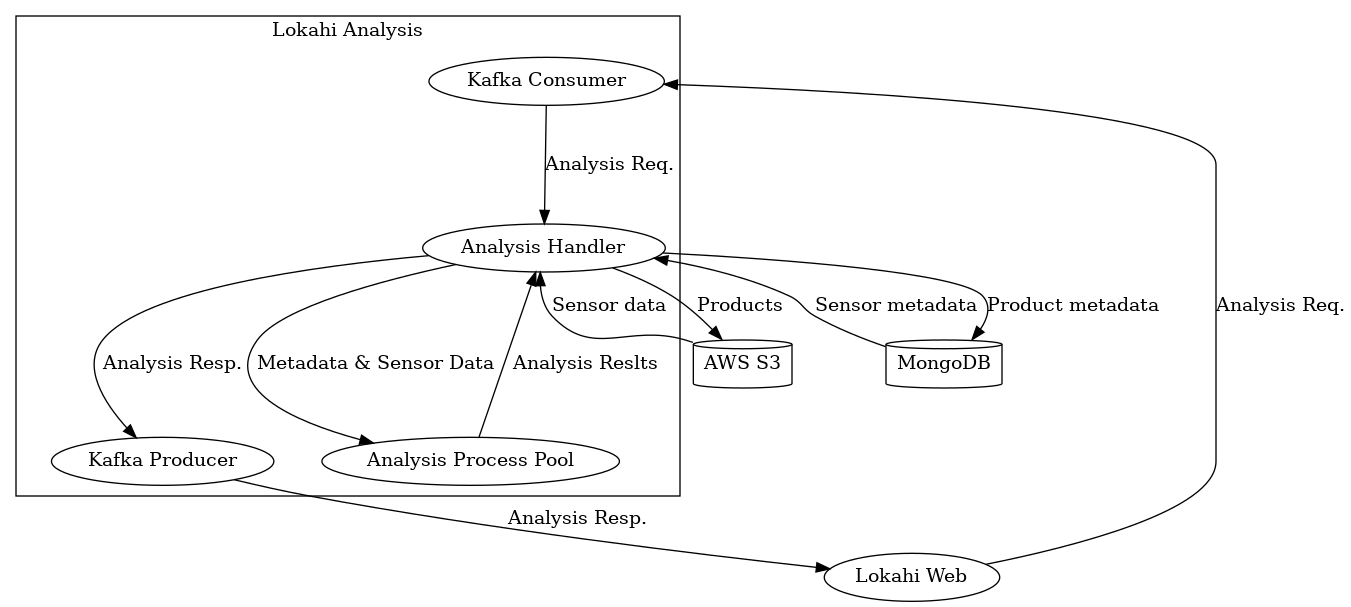
\includegraphics[width=\linewidth]{figures/analysis_architecture.png}
	\caption{Lokahi Analysis Architecture}
	\label{fig:analysis_architecture}
\end{figure}

\subsection{Lokahi Web}\label{subsec:lokahi-web}
Lokahi Web is a web interface that allows users to check the status of their sensors, download sensor data, and generate analysis reports. It also allows administrators to view sensor data usage, send alerts to sensors, and manage users. Lokahi Web is written in Java and powered by the Play Framework. Most functionality in Lokahi Web is provided from metadata stored in the MongoDB and by passing messages band and forth to the analysis service over a Kafka queue.

\subsubsection{Sensor Status}
The main page of Lokahi Web displays a map of currently active sensors (that the logged in user can access) and displays a list of those sensors sorted by distance from the users current location. This data is obtained by loading metadata from the database. An example if this interface is displayed in Figure~\ref{fig:lweb_main}.

\begin{figure}
	\centering
	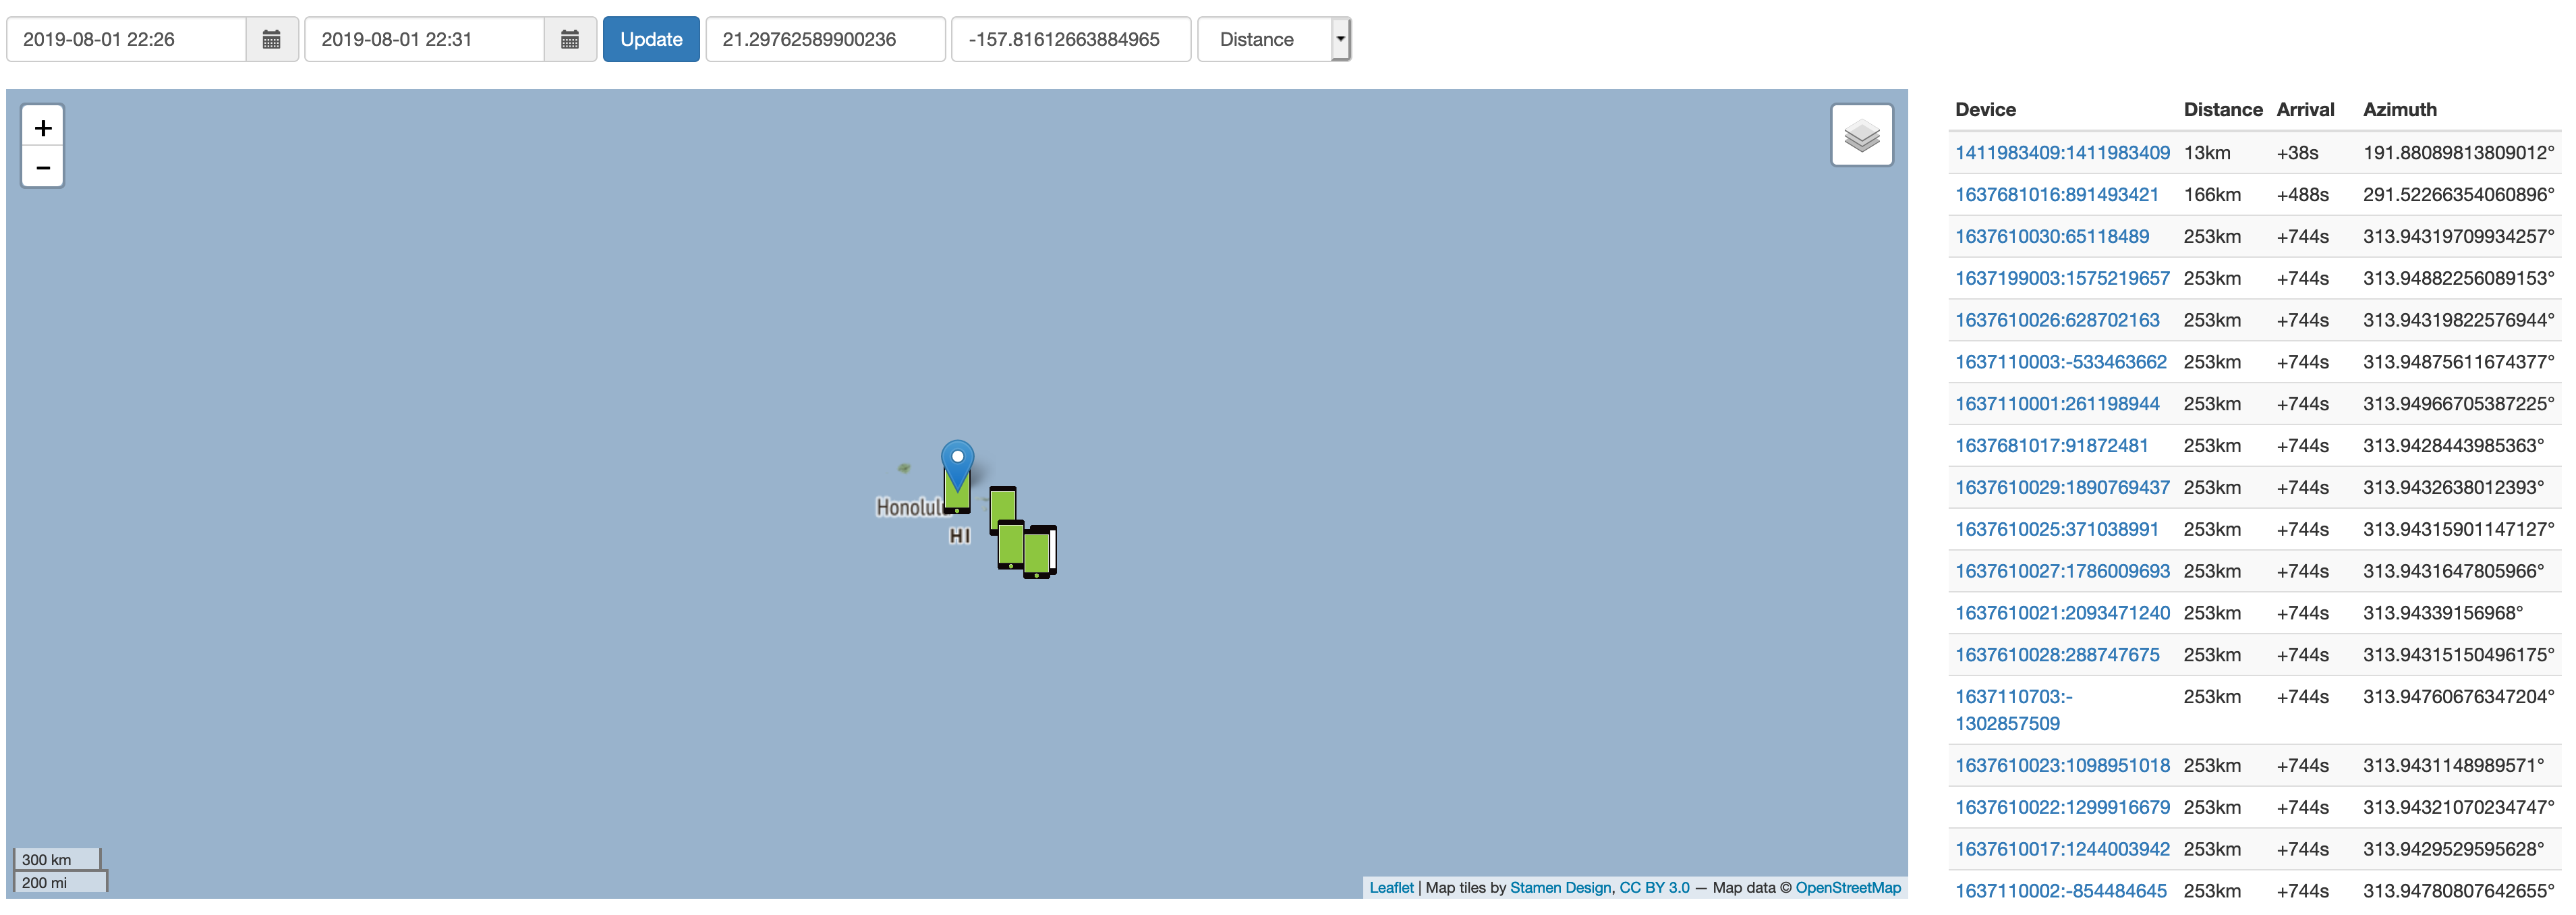
\includegraphics[width=\linewidth]{figures/lweb_main.png}
	\caption{Lokahi Web Main Page}
	\label{fig:lweb_main}
\end{figure}

The ``Active Devices" page lists all active devices that the logged in user can access as well as some metadata about those sensors. This data is loaded as metadata from the database. An example of this page is displayed in Figure~\ref{fig:lweb_status}.

\begin{figure}
	\centering
	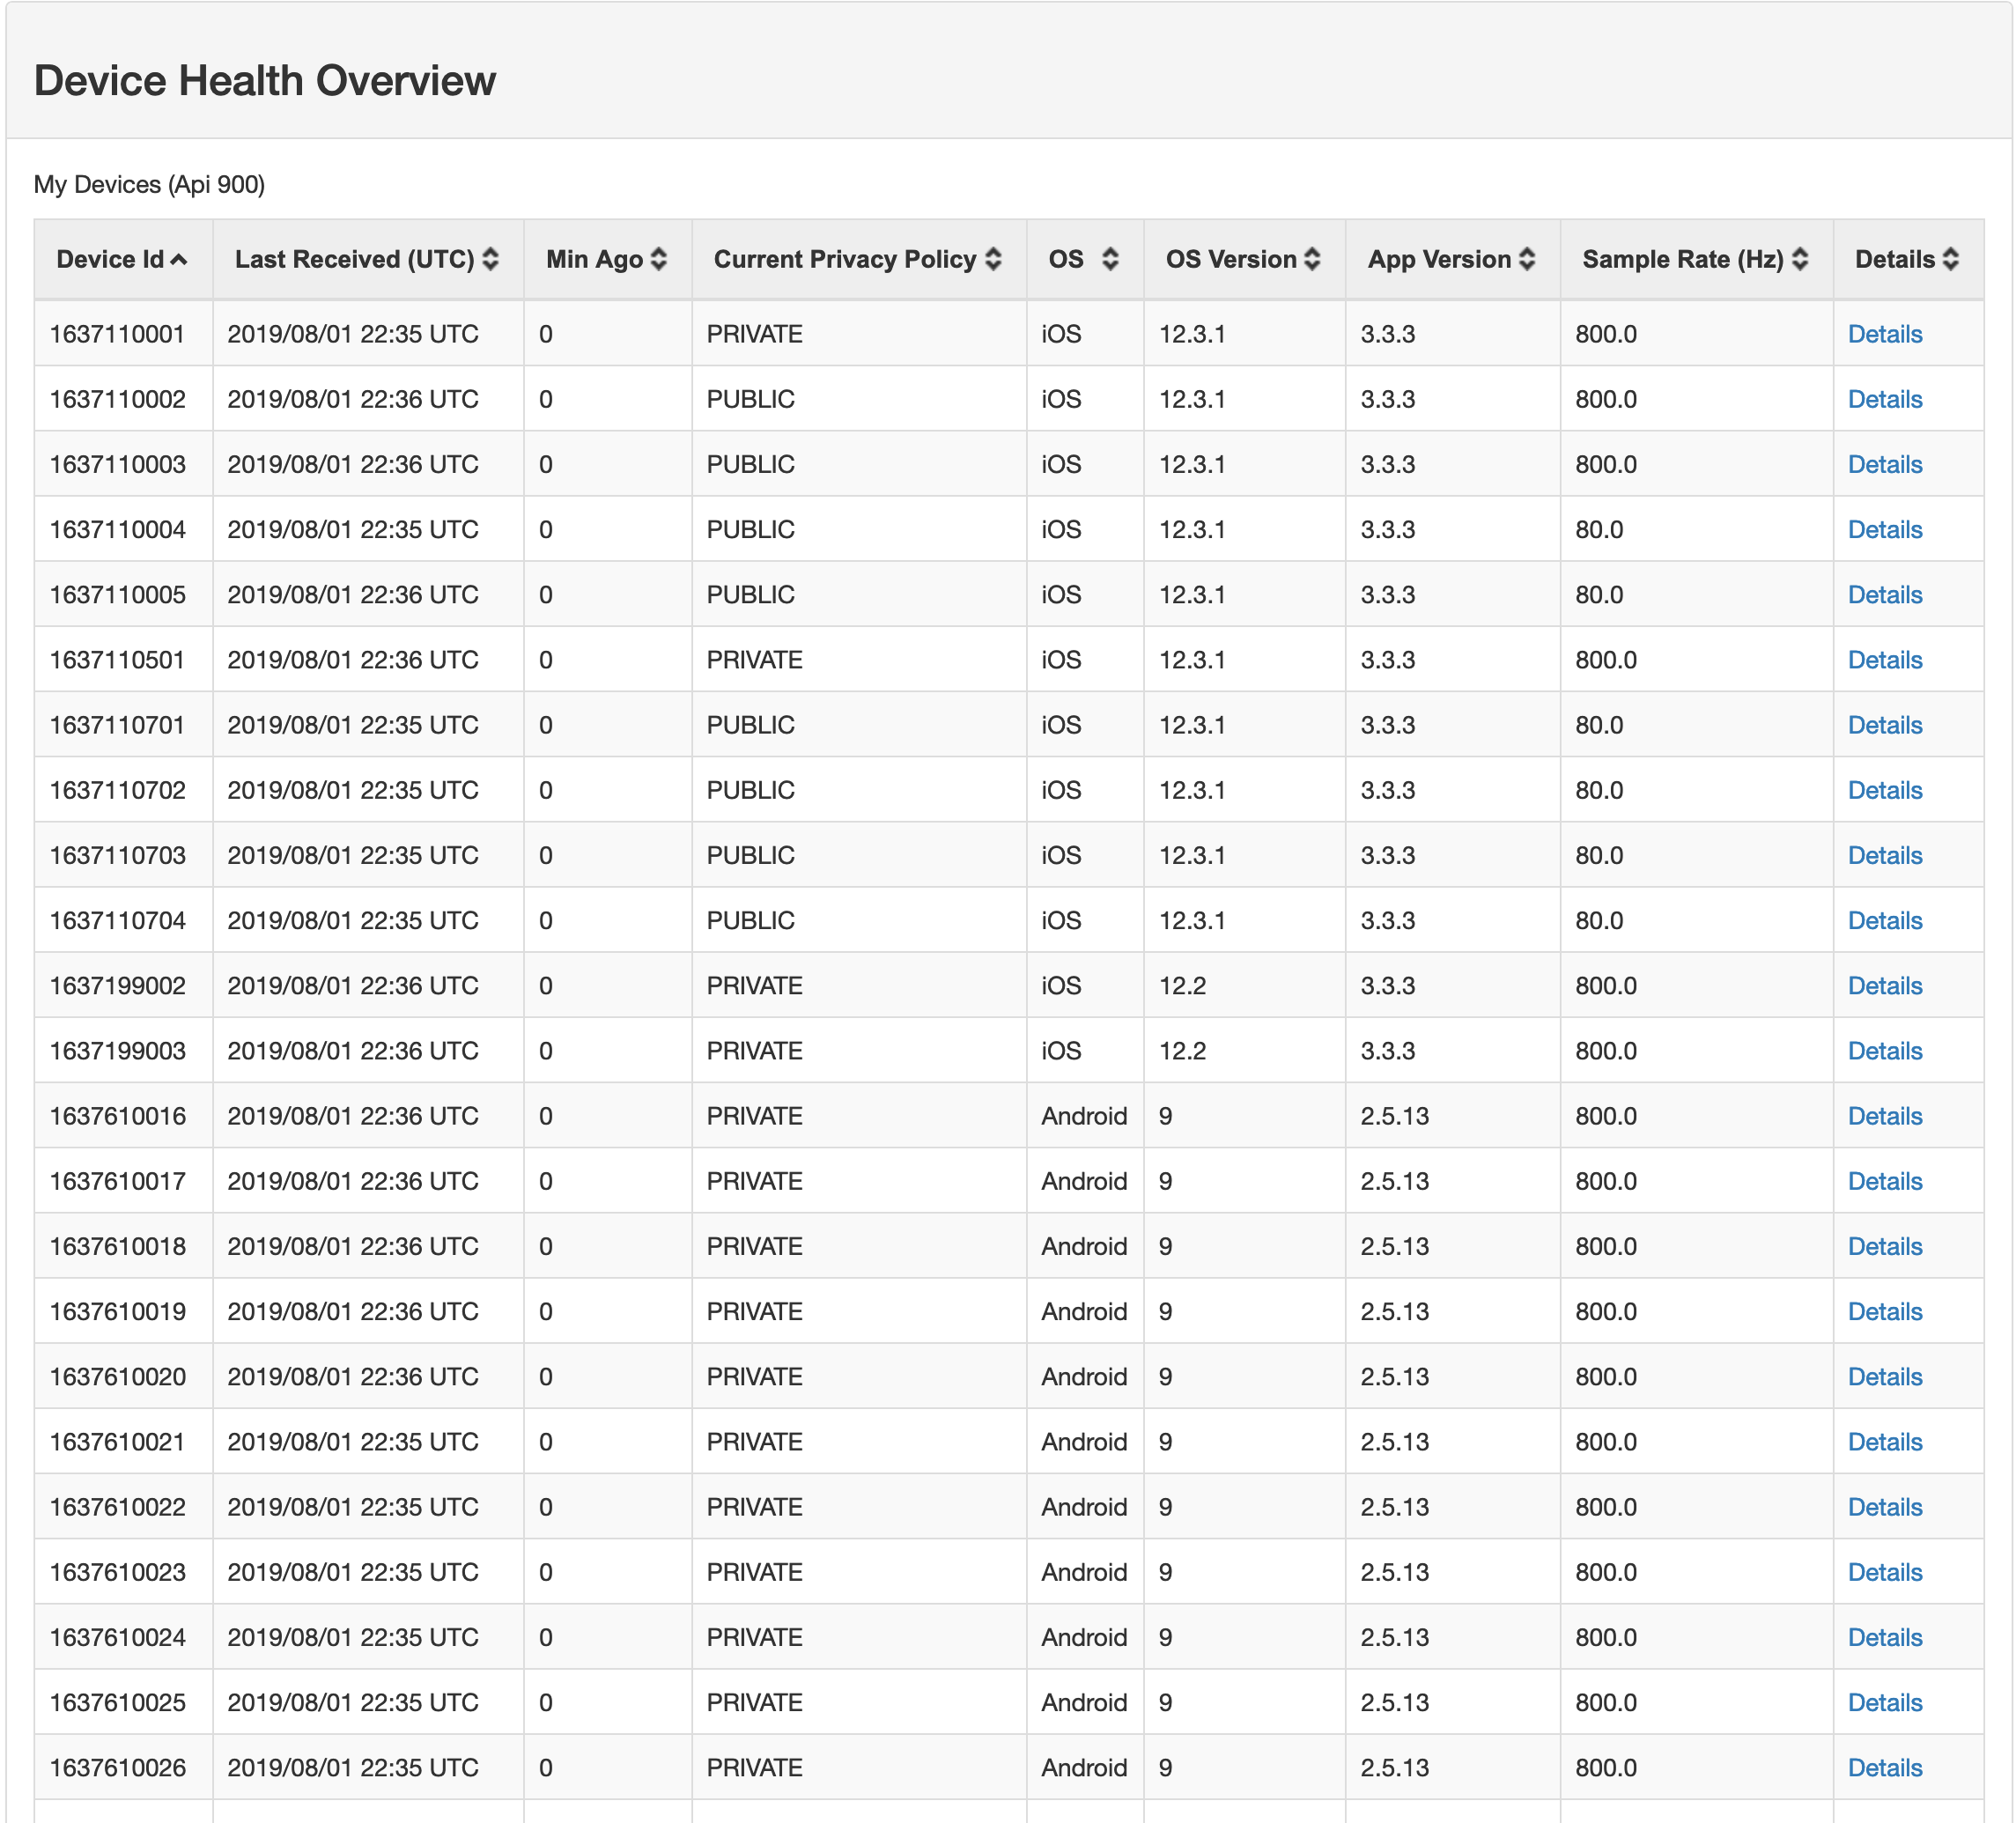
\includegraphics[width=\linewidth]{figures/lweb_status.png}
	\caption{Active Devices}
	\label{fig:lweb_status}
\end{figure}

It's possible to drill into the details of an individual device by clicking the ``Details" link on the ``Active Devices" page. The detailed device status includes a map of the location of the device, the device activity over the past hour and past day, metadata details, and real-time plots for microphone, barometer, location, and time synchronization This data is loaded as metadata from the database and also real-time sensor payload data is retrieved from the real-time Kafka ring buffer. An example of detailed device status is provided in Figure~\ref{fig:lweb_detail}.

\begin{figure}
	\centering
	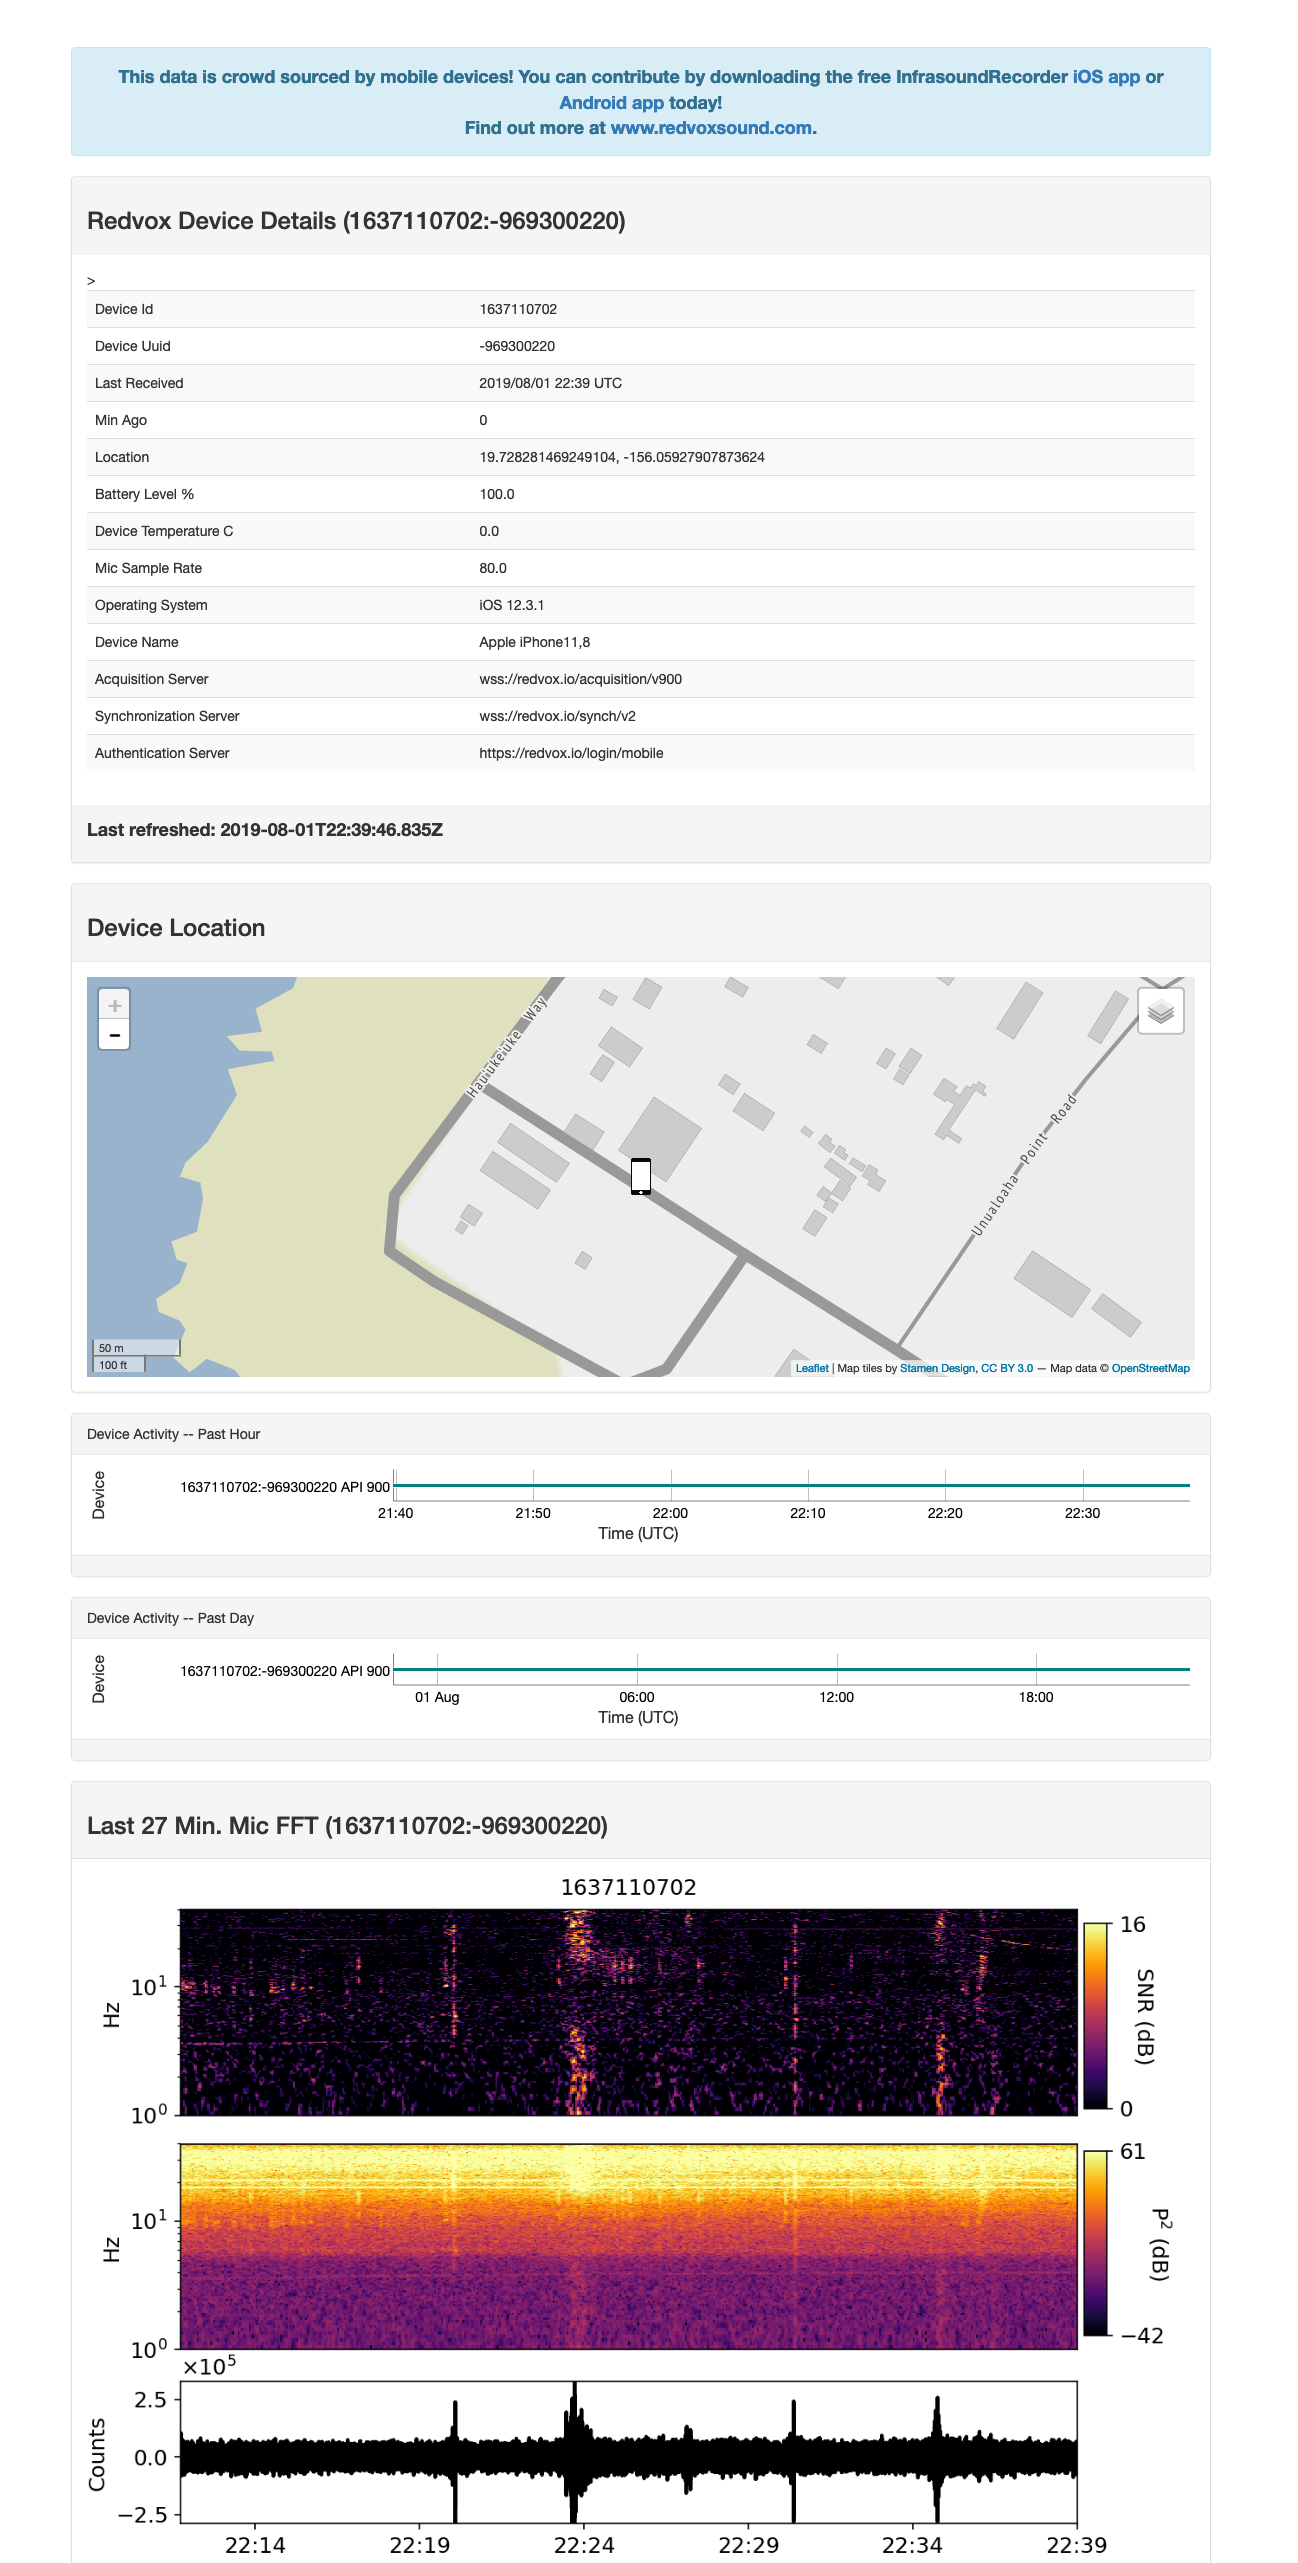
\includegraphics[width=0.7\linewidth]{figures/lweb_detail.png}
	\caption{Detailed Device Status}
	\label{fig:lweb_detail}
\end{figure}

Users are able to create groups of devices based on geo-location by defining a bounding box. Then all sensors that are within that bounding box will appear in that user created group. This allows users to view the status of multiple devices at one time for a specific geographic location. This data is stored as metadata in the database. An example of the group creation interface is displayed in Figure~\ref{fig:lweb_groupcreate}.

\begin{figure}
	\centering
	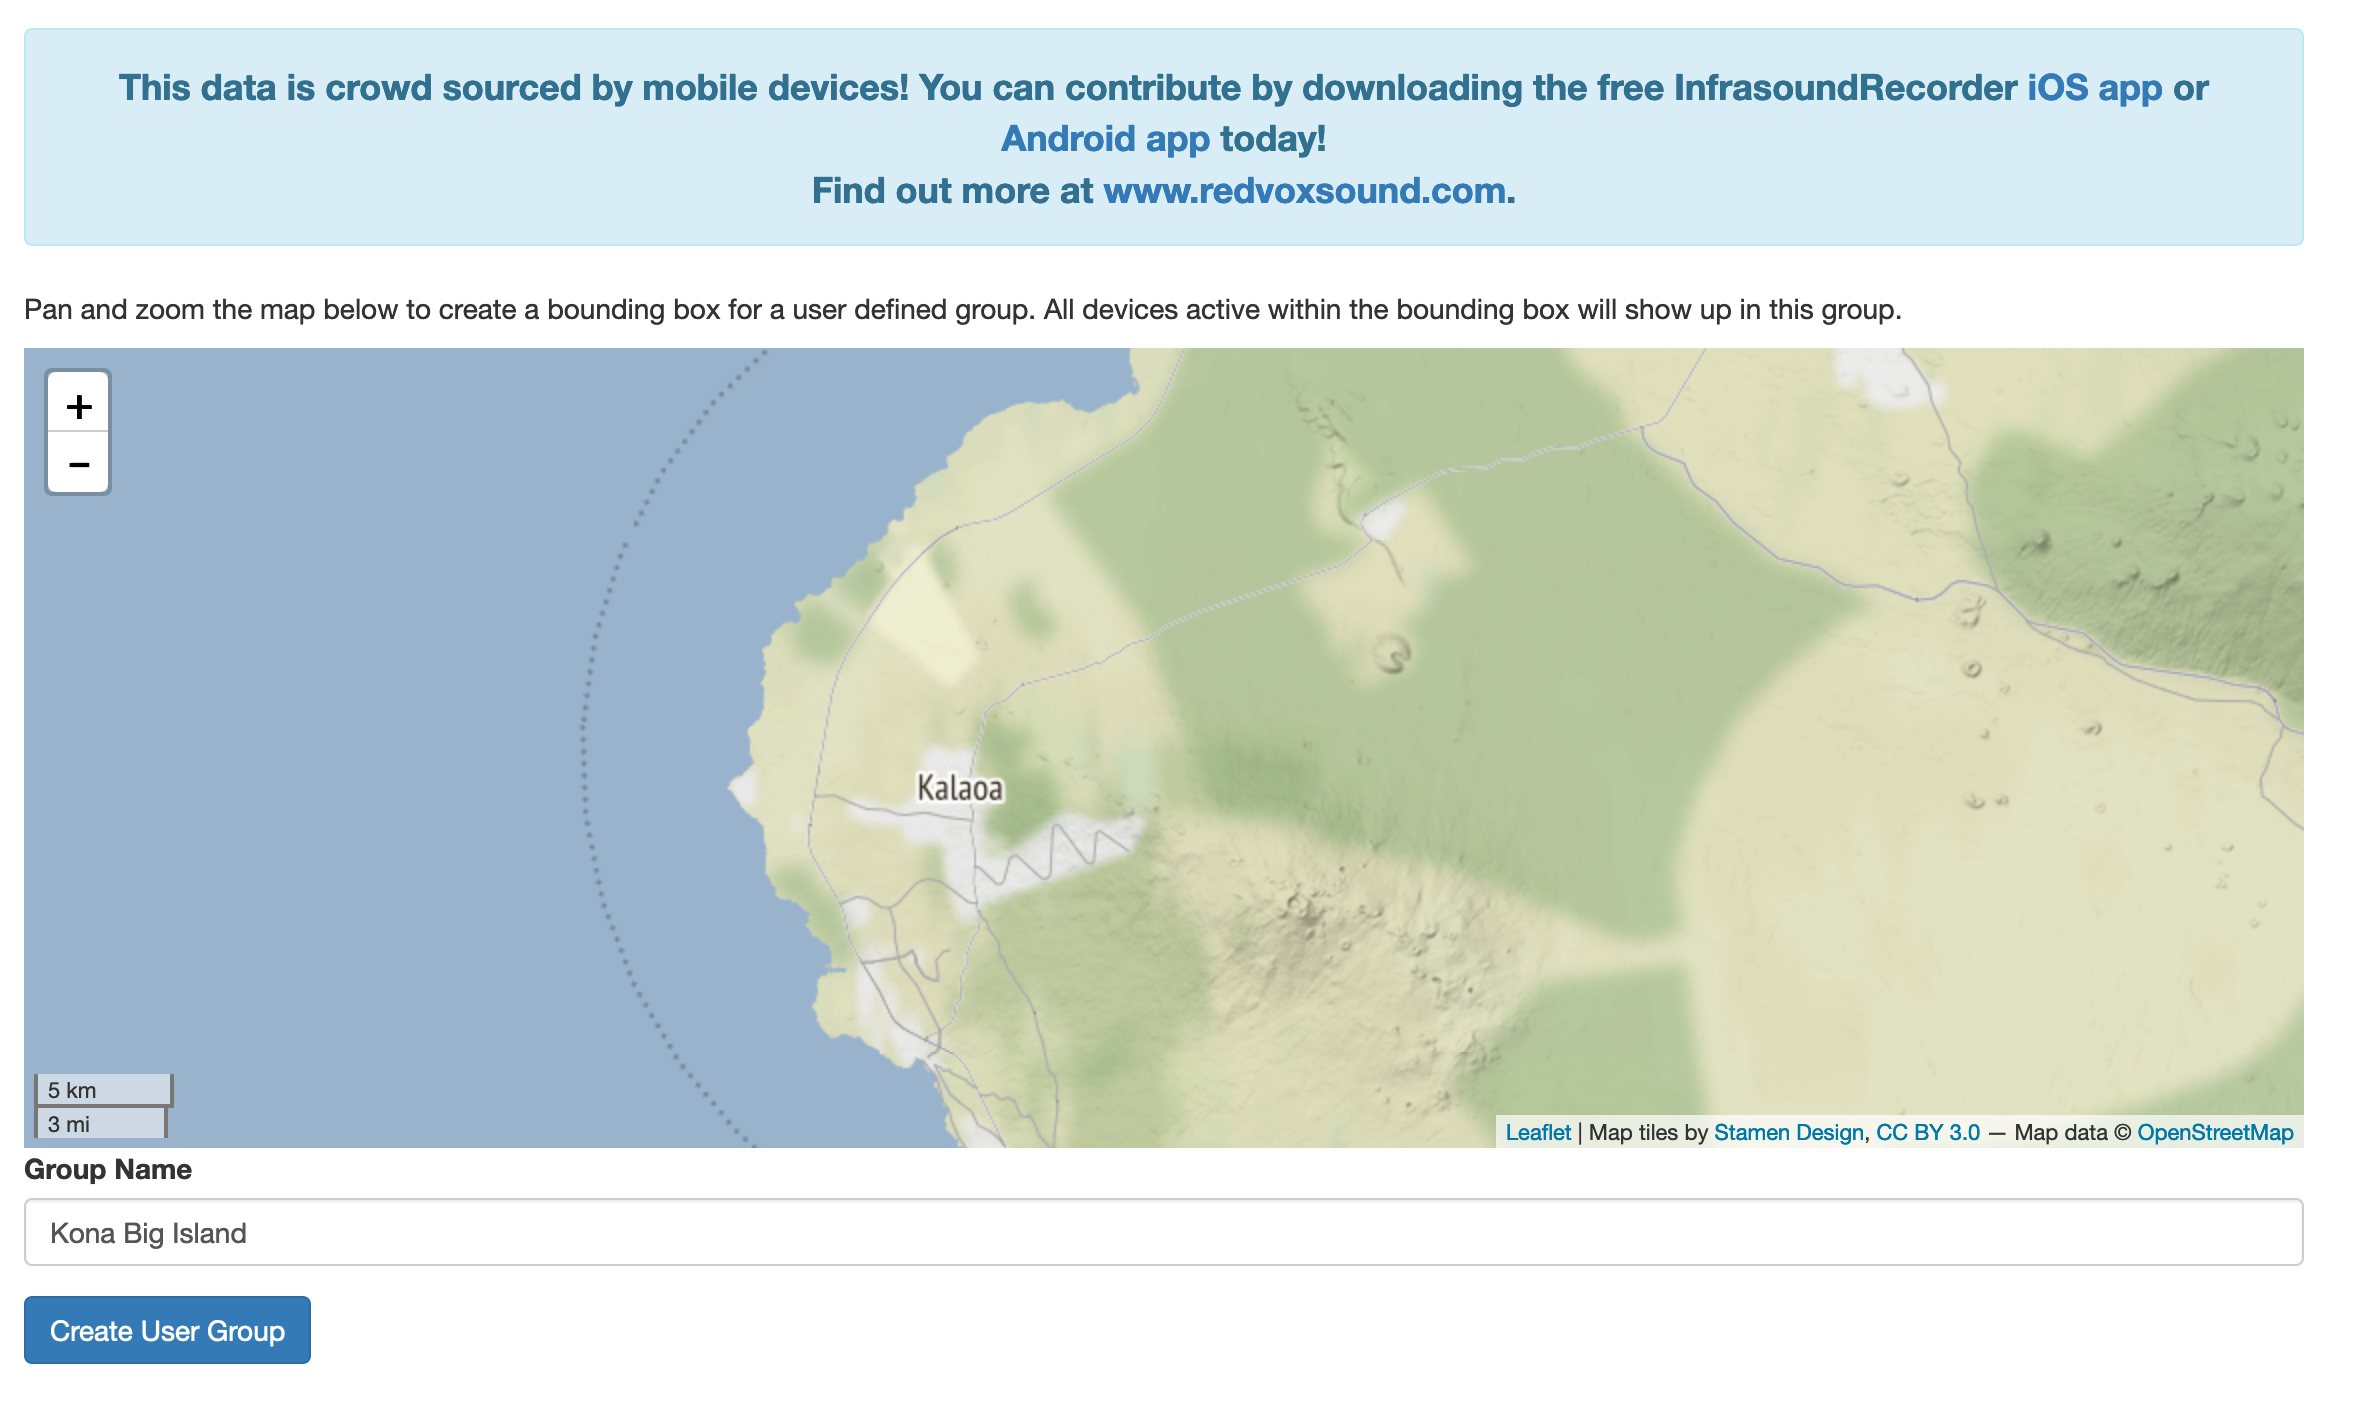
\includegraphics[width=0.7\linewidth]{figures/lweb_groupcreate.png}
	\caption{Sensor Group Creation}
	\label{fig:lweb_groupcreate}
\end{figure}

Once a group is created, you can then view the status of all devices in that group by going to the group's page. This page will display device activity for each device over the past hour and provides a quick interface for generating an analysis report from that specific grouping of devices. This data is a combination of metadata and real-time data from the Kafka buffer. An example of this is displayed in Figure~\ref{fig:lweb_group}.

\begin{figure}
	\centering
	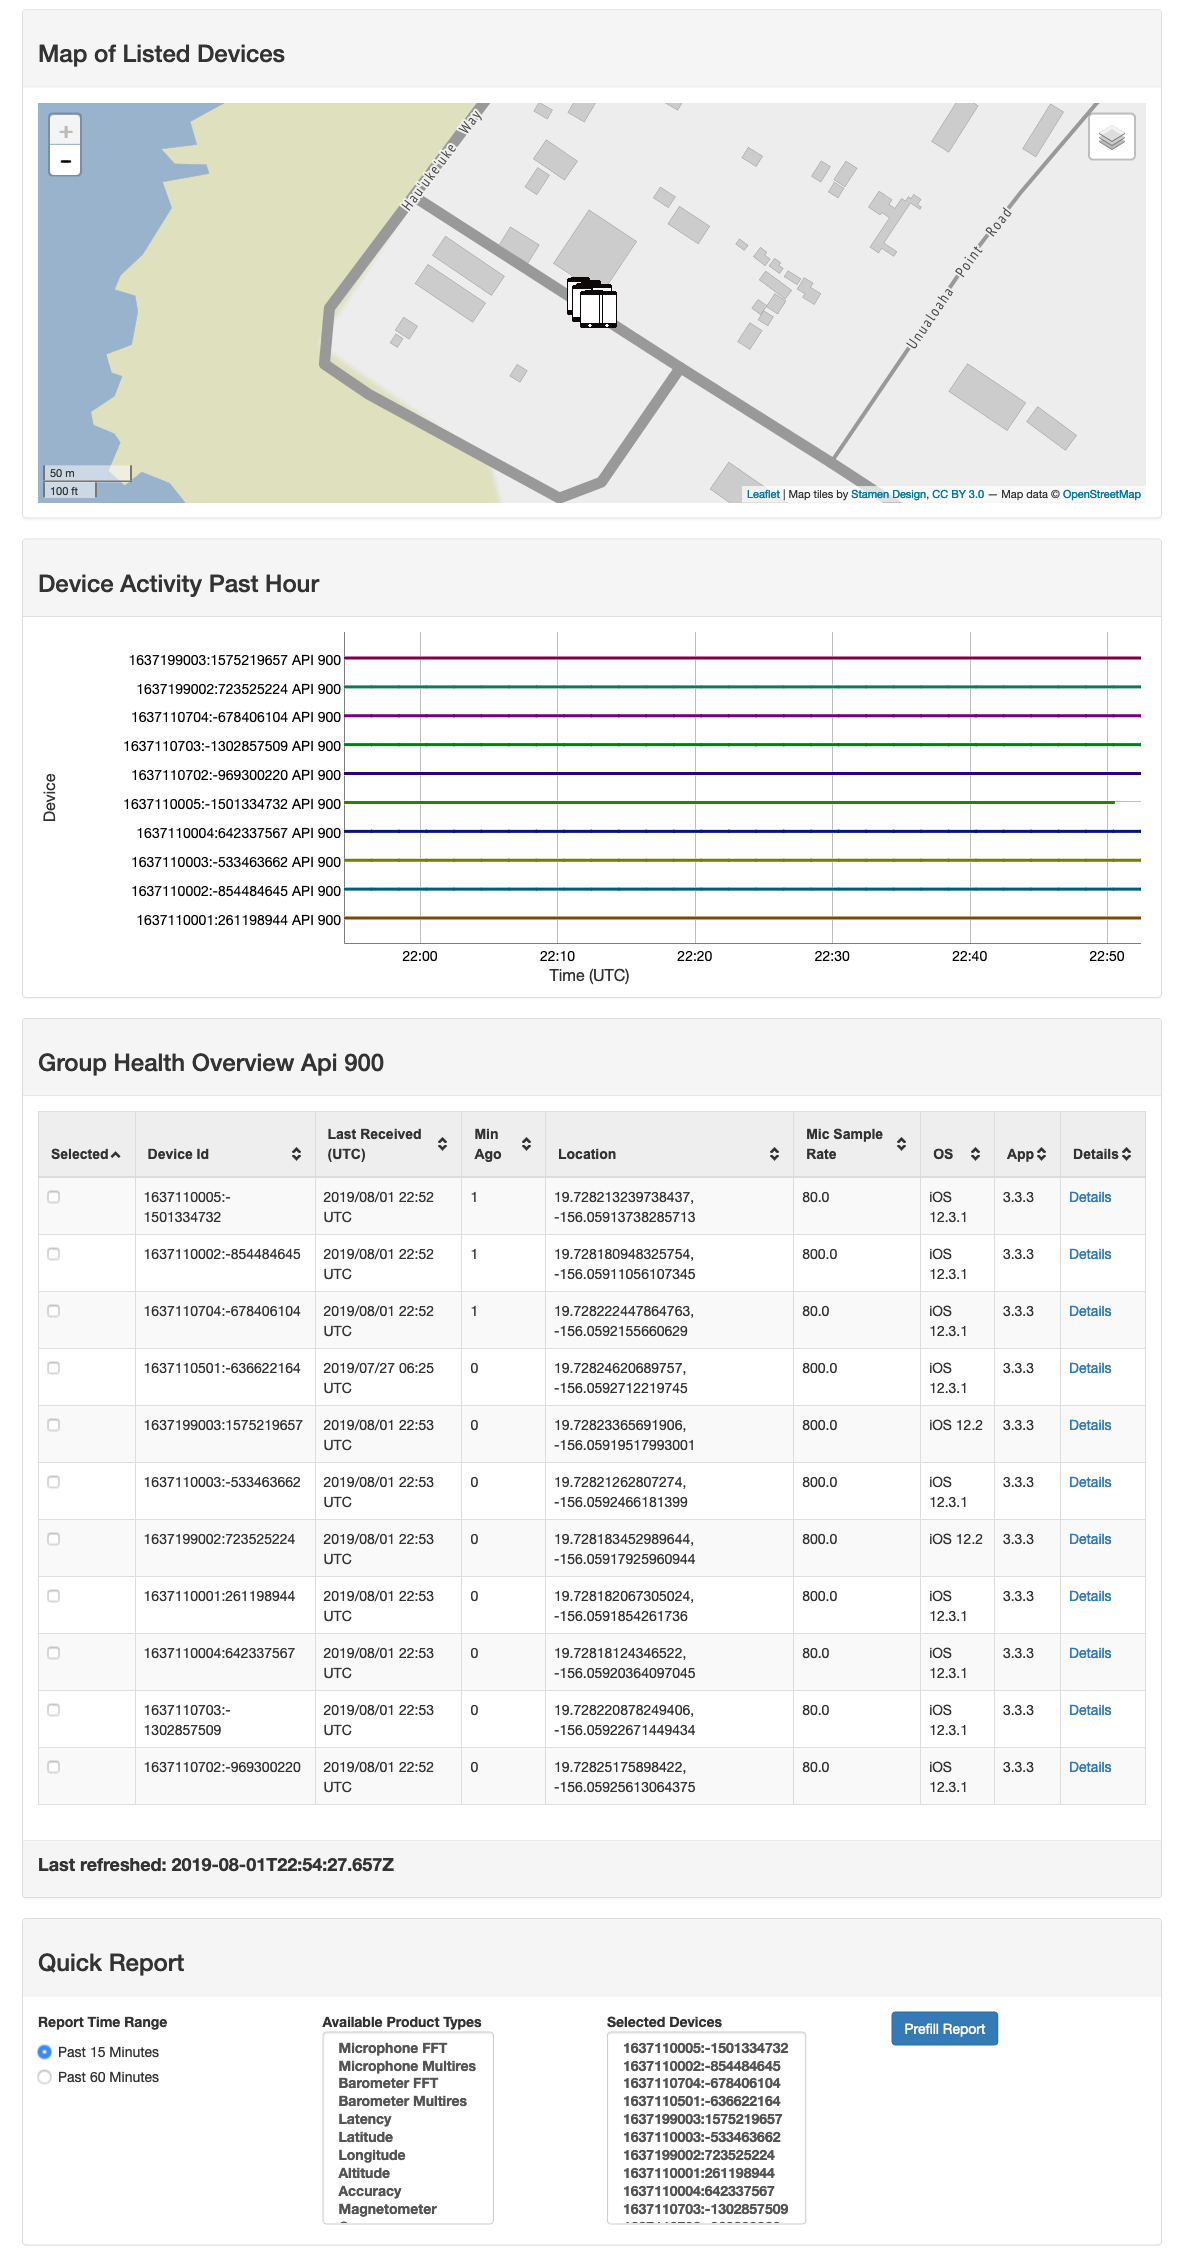
\includegraphics[width=0.7\linewidth]{figures/lweb_group.png}
	\caption{Sensor Group Status}
	\label{fig:lweb_group}
\end{figure}

\subsubsection{Data Explorer}
The ``Data Explorer" page provides a custom built interface that displays details of individual data packets as they arrive. This is useful for debugging and ensuring that the sensors are sending what the users expect the sensors to be sending.

This page displays information loaded from the database. If a sensor channel is selected, then the payload is received from AWS S3 and displayed on this page using a custom JavaScript plotter. This page also allows users to download individual data packets or export payloads as CSV\@.

An example of the data explorer is provided in Figure~\ref{fig:lweb_dataexplorer} and shows the waveform from a selected microphone channel.

\begin{figure}
	\centering
	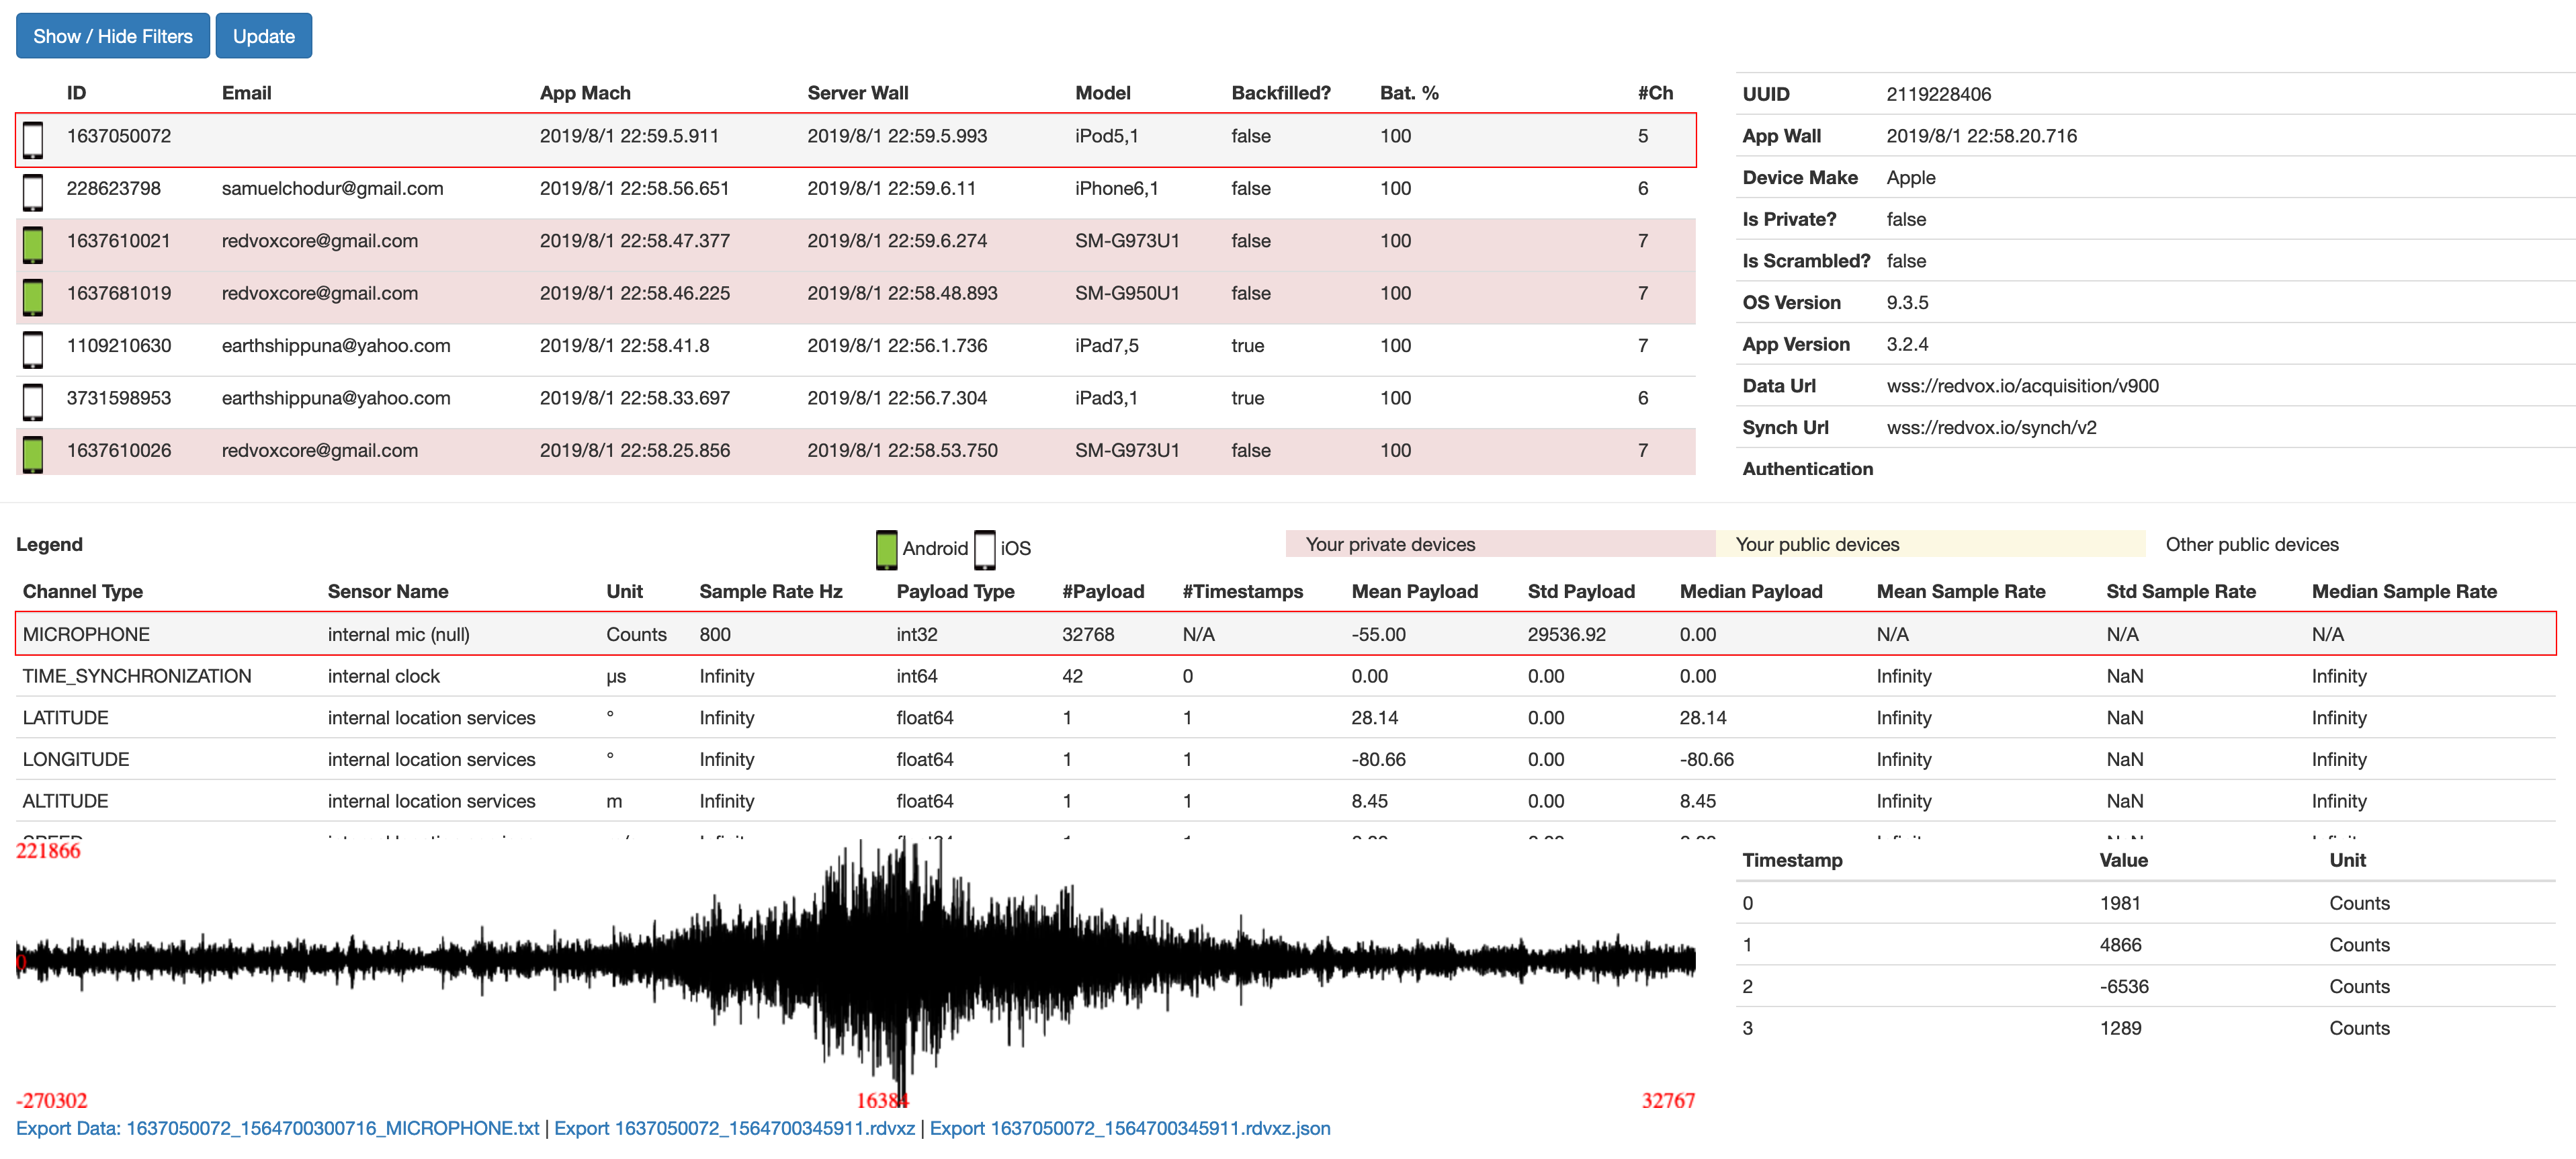
\includegraphics[width=0.7\linewidth]{figures/lweb_dataexplorer.png}
	\caption{Data Explorer Interface}
	\label{fig:lweb_dataexplorer}
\end{figure}

Data within the explorer can be filtered by device id, device owner, time window, device make/model, os version, app version, microphone sampling rate, onboard sensors, and privacy status.

\subsubsection{Analysis Reports}
The main component of Lokahi Web is its report generation functionality. This functionality allows users to generate analysis reports from sensors that they can access with configurable time windows and sensor feature selection. Users can edit report metadata, rerun reports with new parameters, and share their reports with other Lokahi Web users. Administrators can set reports as featured reports which then make those reports available to the general public.

The report generation interface allows users to select devices, time windows, and which products should be generated. When a user selects a time window and an estimated signal source location, the interface automatically lists available sensors for that time window sorted by distance from the signal source. This makes it easy for users to determine which sensors to include in the report by seeing how far sensors are from estimated signal sources.

When a user has selected all configuration options, a report analysis request is serialized with Protocol Buffers and sent to the Lokahi Analysis service where the report is actually generated. Once the report is generated, the analysis service sends a response back to Lokahi Web and Lokahi Web displays the newly minted report.

The report interface also allows users to download raw sensor data for the selected devices over the selected time range.

An example of the report interface is provided in Figure~\ref{fig:lweb_reportcreate}.

\begin{figure}
	\centering
	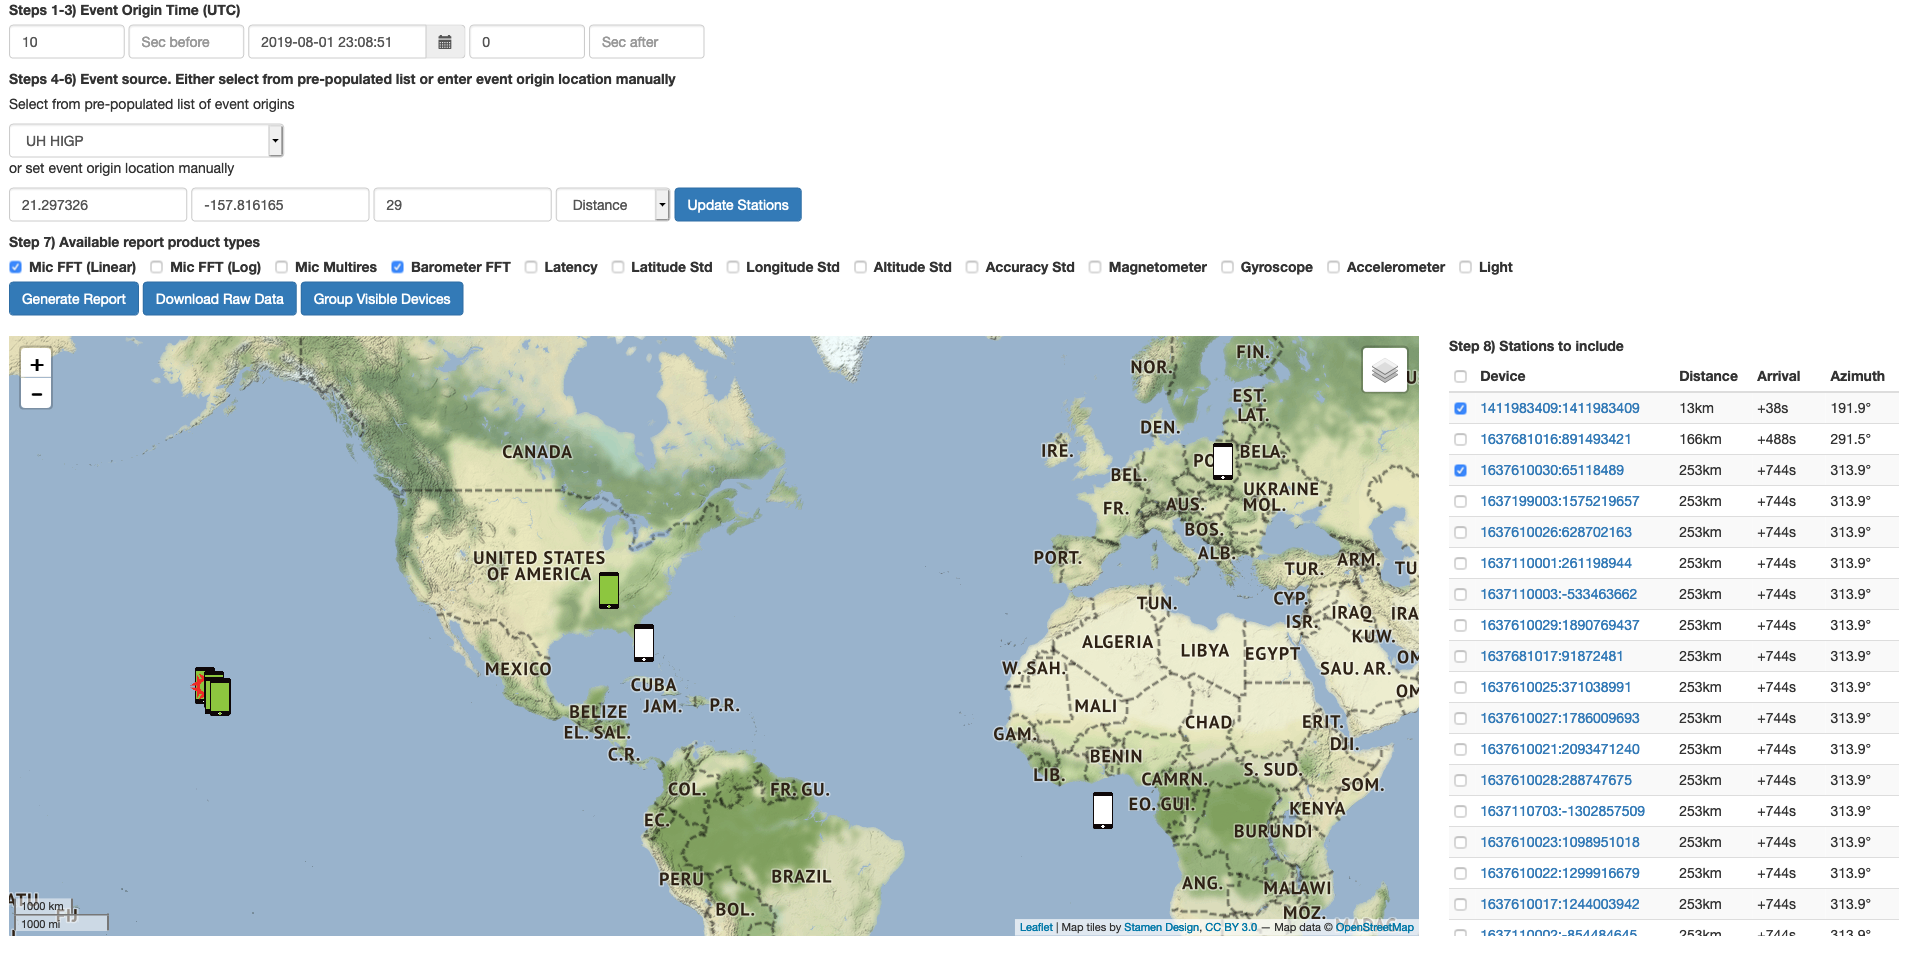
\includegraphics[width=0.7\linewidth]{figures/lweb_reportcreate.png}
	\caption{Report Creation Interface}
	\label{fig:lweb_reportcreate}
\end{figure}

An example of a report with one device is provided in Figure~\ref{fig:lweb_report}.

\begin{figure}
	\centering
	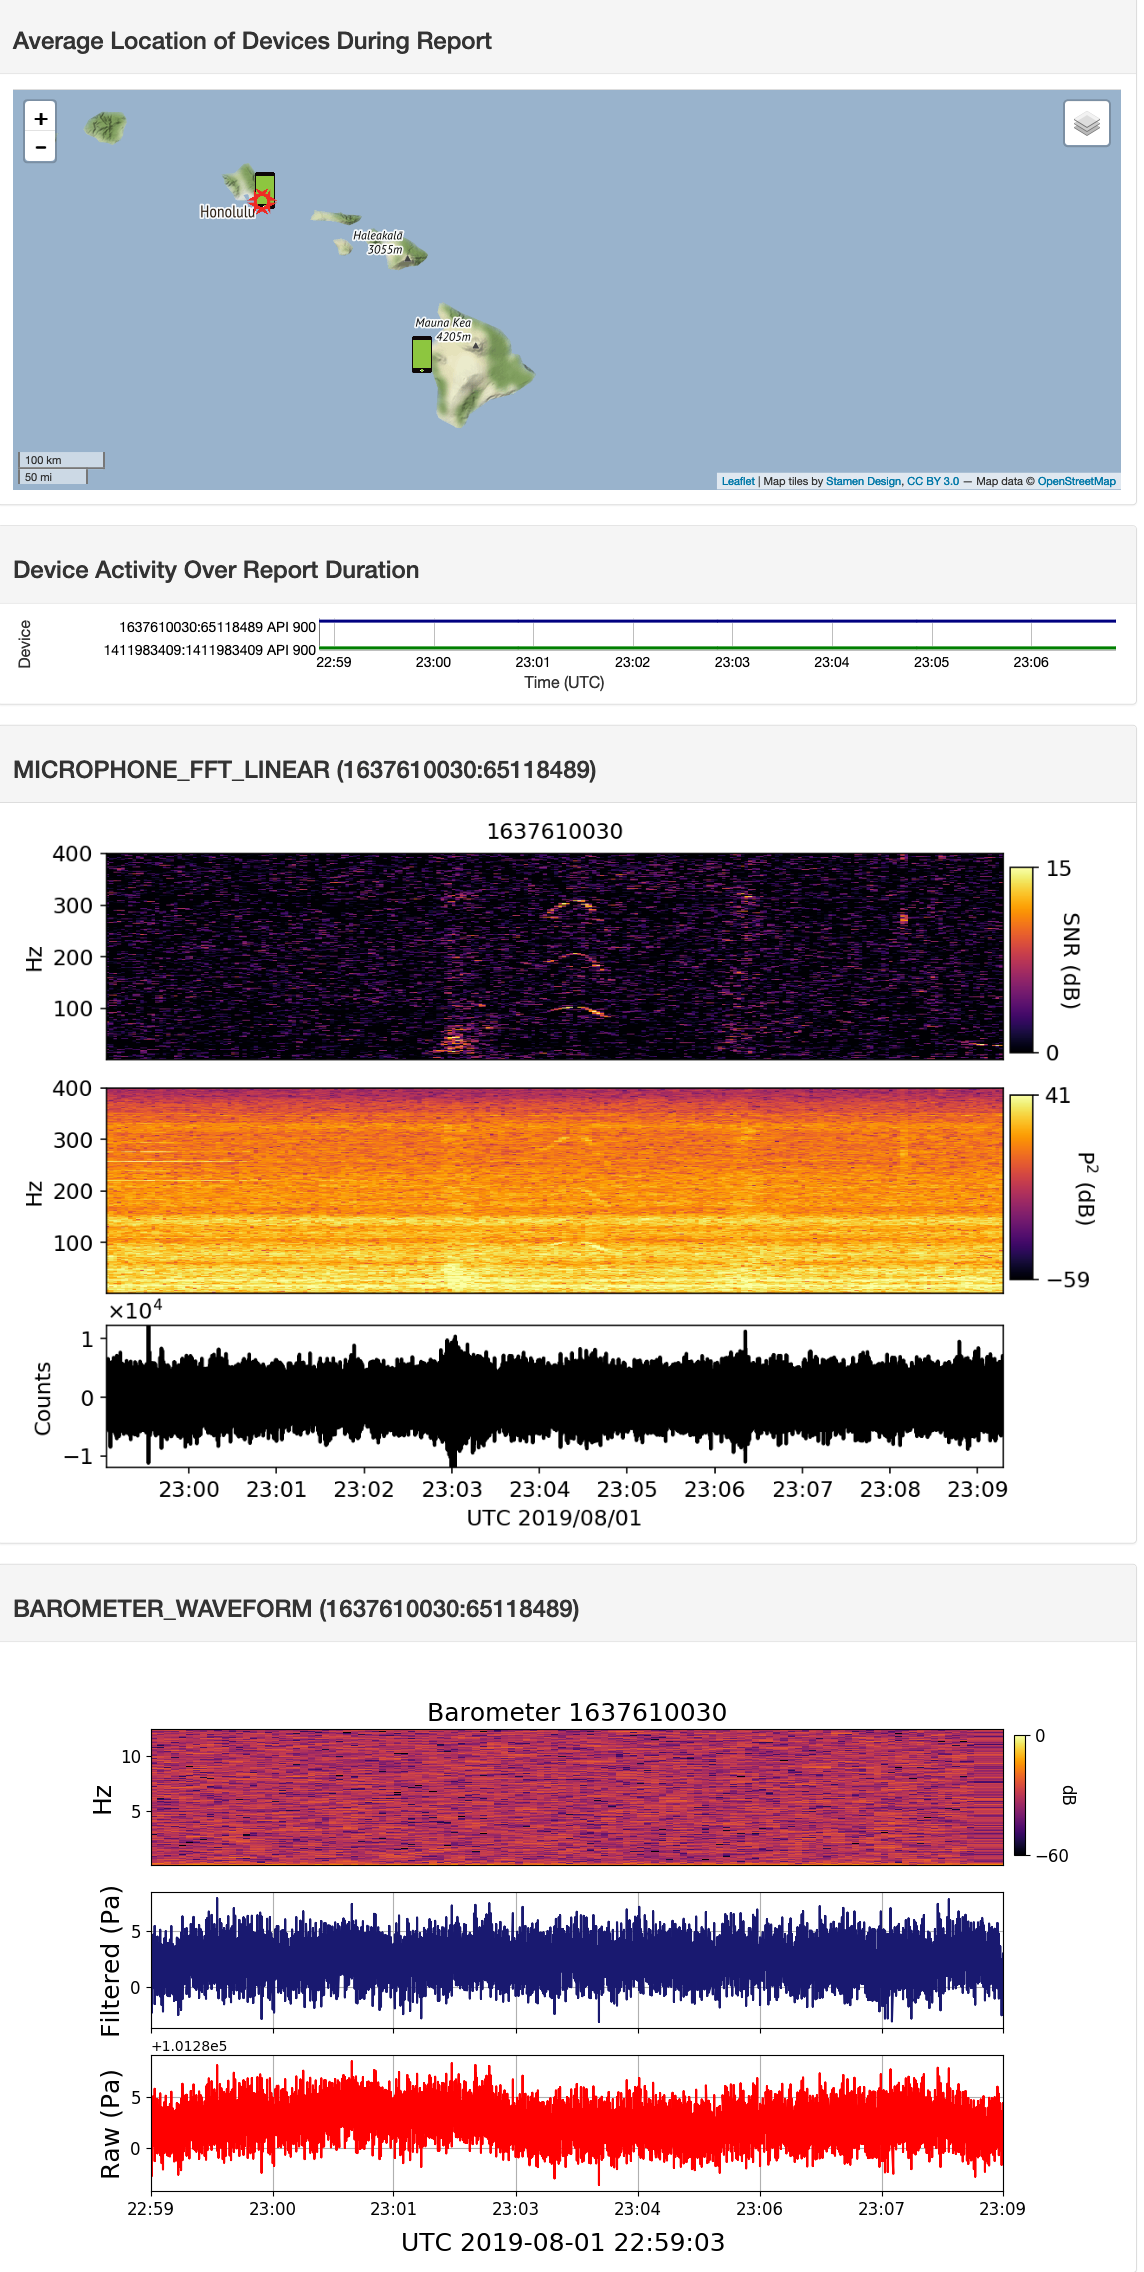
\includegraphics[width=0.7\linewidth]{figures/lweb_report.png}
	\caption{Lokahi Web Report}
	\label{fig:lweb_report}
\end{figure}

Users have the ability to sanitize reports. This removes timing, device, and location information from the reports and instead displays these values as relative offsets. For example, time is offset as seconds since 0 and location is offset as distance from an unknown source. This allows users to share sensitive reports while removing identifying information.

Each report also has a link that allows users to download the raw sensor data that was used in generating the report.

The metadata of each report can also be directly edited. This includes adding Annotation Phenomena to classified Incidents. This is fundamental for Lokahi's goals of building up a labeled dataset for future machine learning endeavors.

Finally, there is a ``Print Version" interface of reports that removes some of the metadata, rearranges the maps and plots for printing or distribution.

\subsubsection{Global Collection}
The global collection interface shows the last location of every device that Lokahi has ever received. This interface is useful for showing sensor deployment adoption. This interface is shown in Figure~\ref{fig:lweb_global}.

\begin{figure}
	\centering
	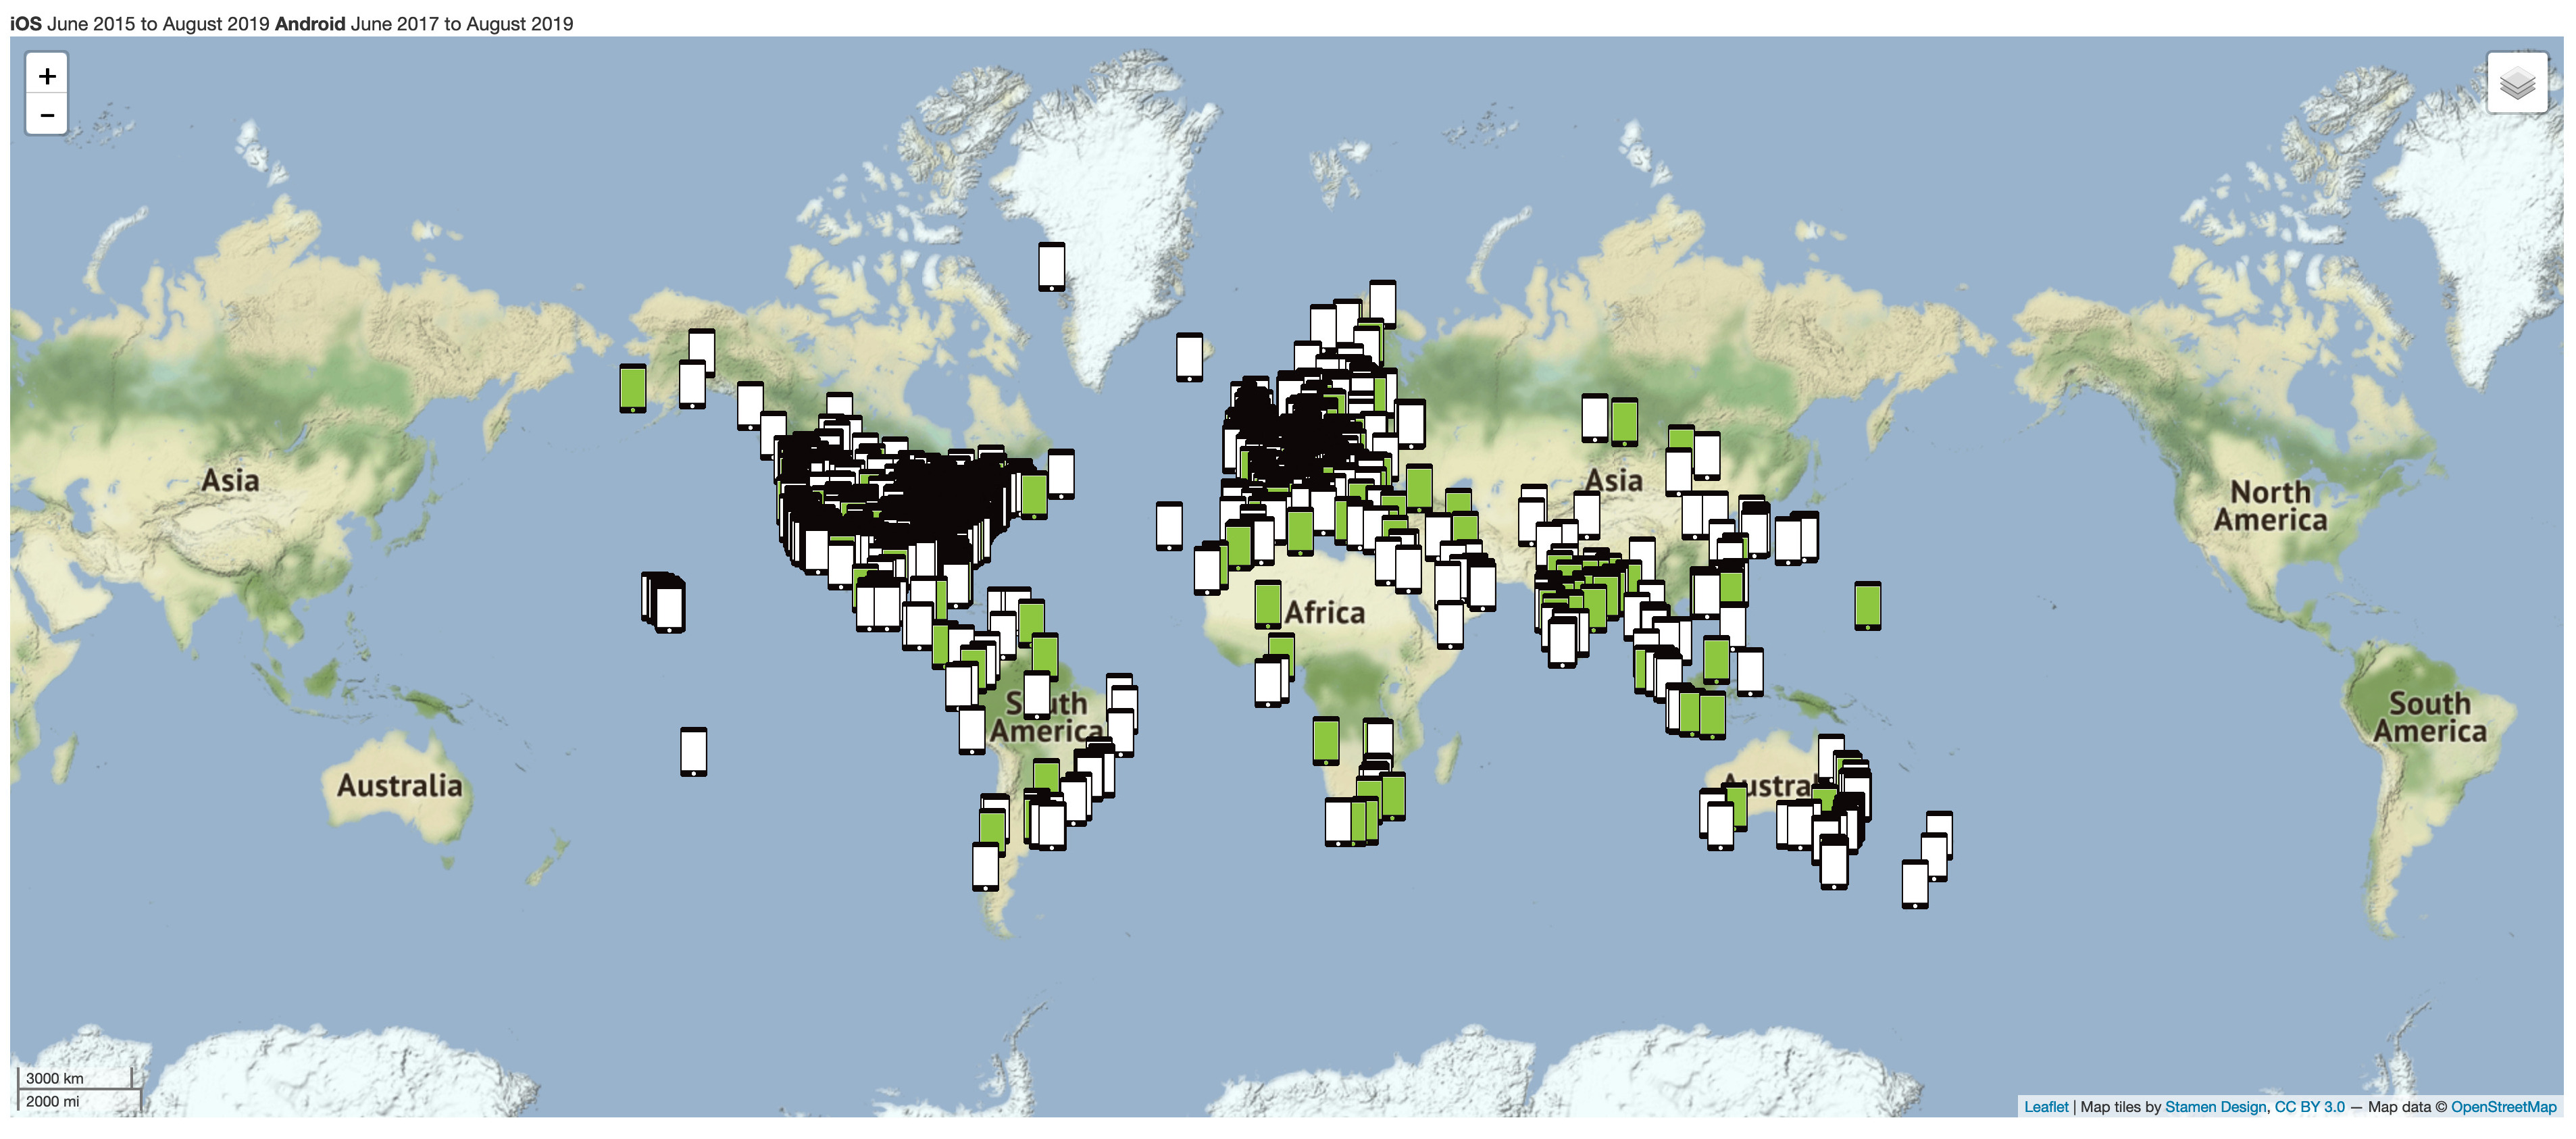
\includegraphics[width=0.7\linewidth]{figures/lweb_global.jpg}
	\caption{Lokahi Global Collection}
	\label{fig:lweb_global}
\end{figure}

\subsubsection{Lokahi Geofenced Alerts}
Lokahi utilizes Google's Firebase Cloud Messaging (FCM) to send geofenced alerts to mobile devices. Since we know the location of each device through its metadata, it's possible to define a bounding box in which only devices within that bounding box will receive an alert.

This is useful when we want to alert users of our sensors to specific events and provides a means of producing actionable insights that can increase S2N. As an example, we may wan to collect data on an upcoming SpaceX launch in Florida. We can create a bounding box for all users in the target area and alert them to an upcoming launch and ask them to turn on their sensors for data collection.

The interface for this is provided by ``Lokahi Web". Once an administrator selects their bounding box and supplies their alert message, Lokahi Web uses the FCM API for queuing a message to all sensors in the target area.

An example of the alerting interface is provided in Figure~\ref{fig:fcm}.

\begin{figure}
	\centering
	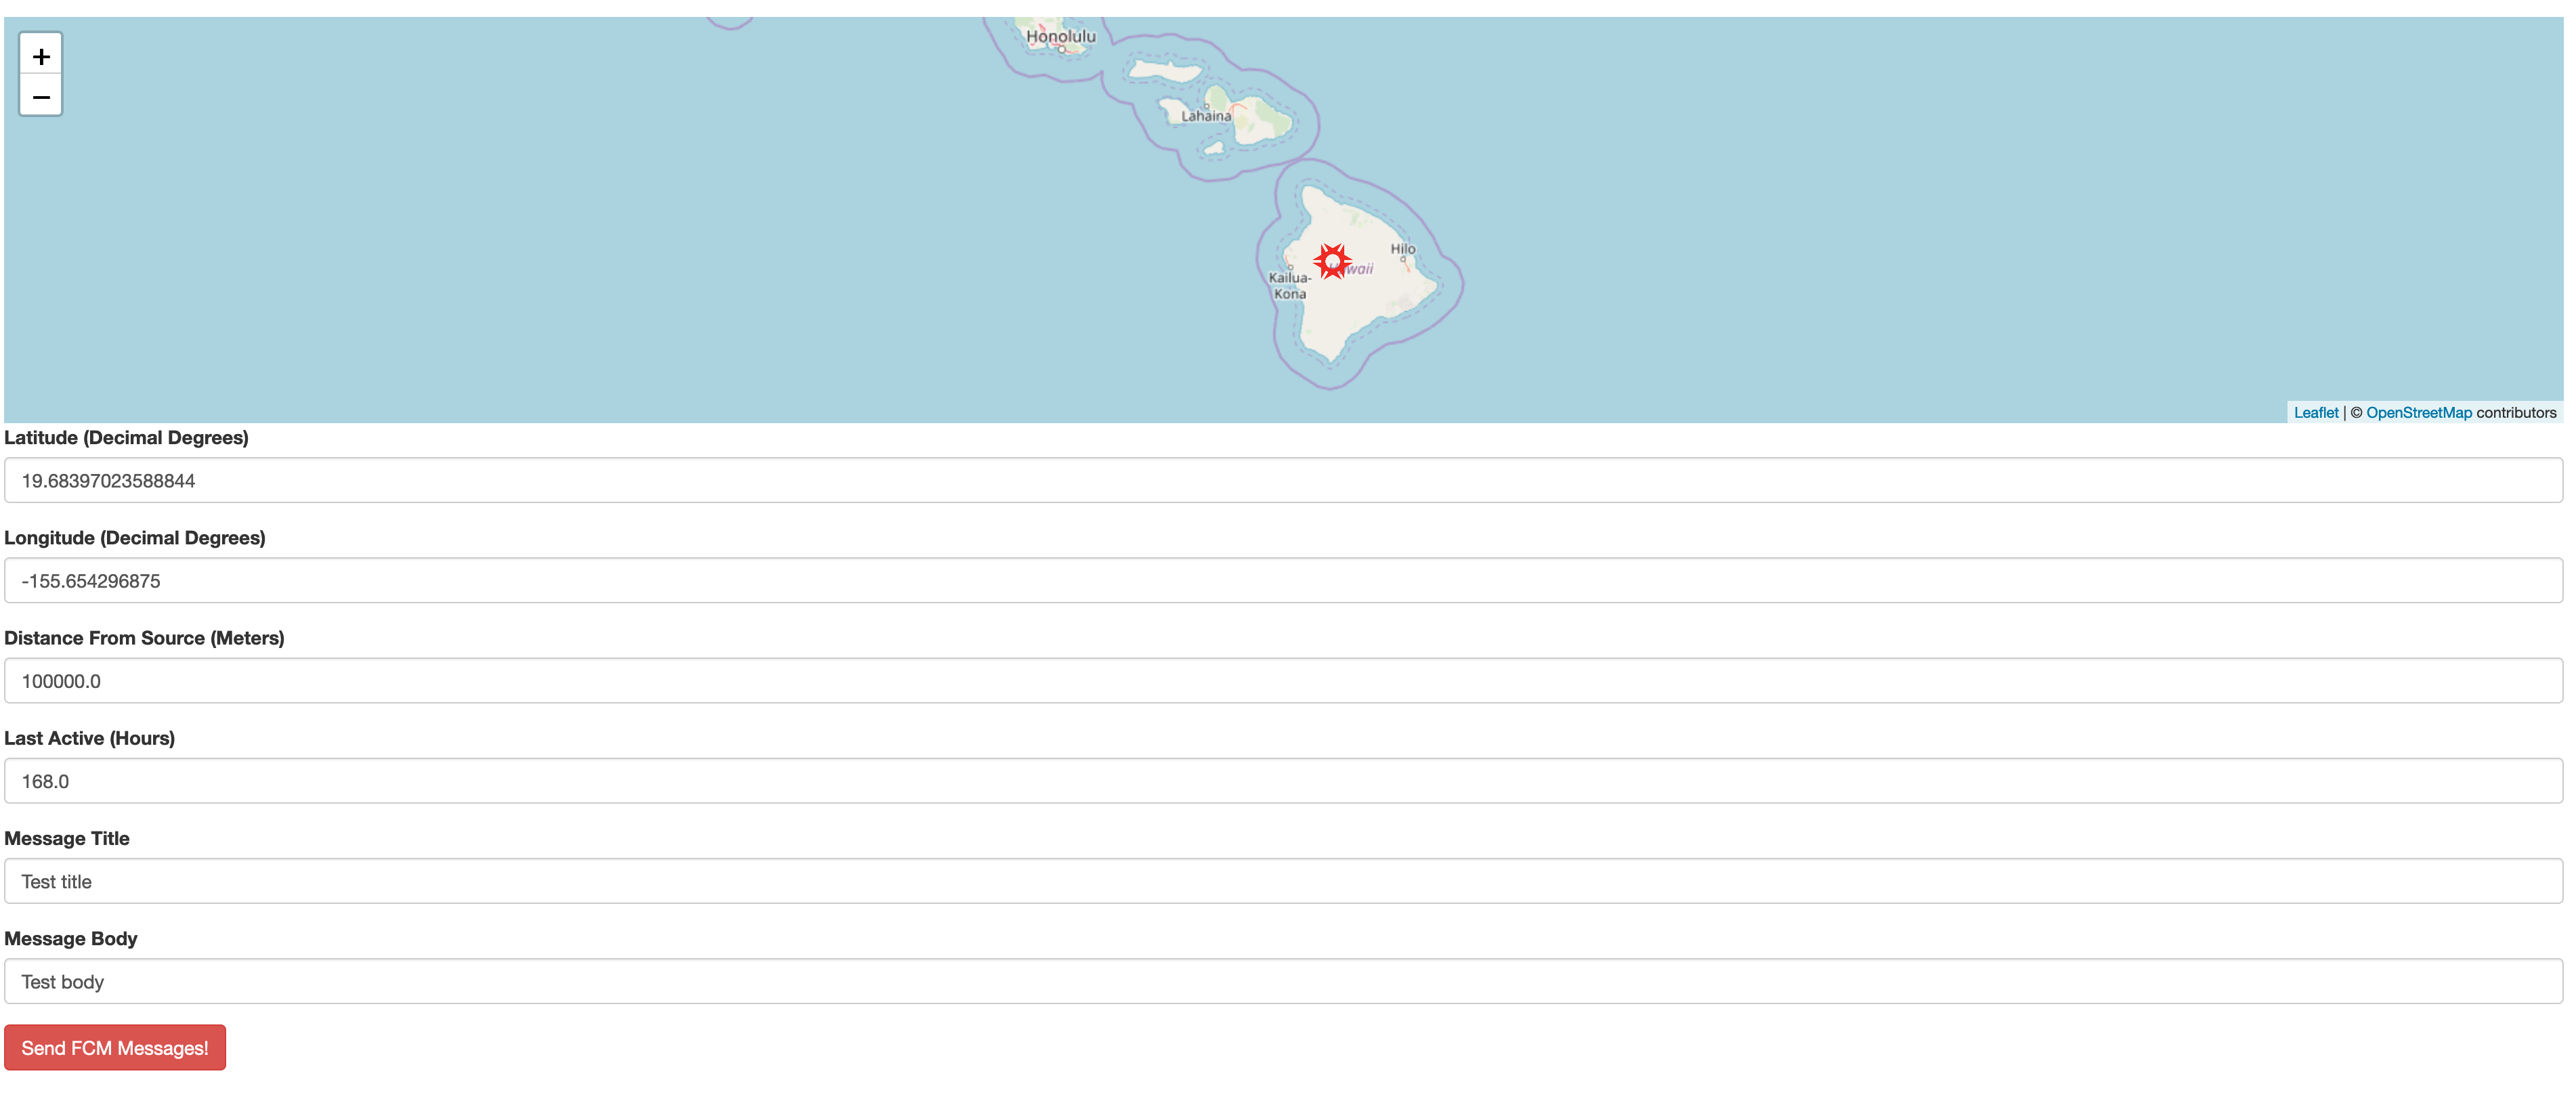
\includegraphics[width=\linewidth]{figures/fcm.png}
	\caption{Geofence Alert Interface}
	\label{fig:fcm}
\end{figure}
